%%% This is one way to your success in fullfilling all HU requirements
%%% 
%%% author:     Heike Prokoph 
%%%        (with the help of google)

\documentclass[%
  open=right,% 
  headsepline,%
  cleardoublepage=empty,%
  listof=totoc,%
  bibliography=totoc,%
  appendixprefix,%
  numbers=noenddot,%
  oneside
]{scrbook}

%%% heads and foots and spacings ... 
\usepackage{scrpage2} 
\pagestyle{scrheadings}
\clearscrplain
\renewcommand*{\headfont}{\normalfont\scshape}
\usepackage{siunitx}
\sisetup{group-separator = {,}}
\sisetup{range-phrase=--,range-units=single}
\usepackage{setspace} % should be called before hyperref!
%\onehalfspacing

%%% define new commands 
\newcommand{\refeq}[1]{Eq.~\ref{#1}}      % equation references
\newcommand{\reffig}[1]{Figure~\ref{#1}}  % figure references
\newcommand{\refsec}[1]{Section~\ref{#1}} % section references
\newcommand{\refch}[1]{Chapter~\ref{#1}}  % chapter references
\newcommand{\refap}[1]{Appendix~\ref{#1}} % appendix references
\newcommand{\reftab}[1]{Table~\ref{#1}}   % table references

%%% change titlepage environment
%%% (attention: title and other metadata are defined later again)
\renewcommand{\maketitle}{\InputIfFileExists{titlepage.tex}{}{}}
\def\mytitle{A Search for Extended Gamma-Ray Emission from the Galactic Center with VERITAS}
\def\myname{Nathan Kelley-Hoskins}
\def\myuni{Humboldt-Universit\"at zu Berlin}
\def\myfaculty{Mathematisch-Naturwissenschaftlichen Fakult\"at}


%%% some stuff to get metadata in PDF/A format 
%%% yes, please write it in again!
\def\Title{A Search for Extended Gamma-Ray Emission from the Galactic Center with VERITAS}
\def\Author{Nathan Kelley-Hoskins}
\def\Subject{}
\def\Keywords{Gamma-Ray astronomy, Non-thermal radiation, galactic center, Cherenkov telescopes systems}


%%% 
\def\convertDate{%
  \getYear
}
{\catcode`\D=12
  \gdef\getYear D:#1#2#3#4{\edef\xYear{#1#2#3#4}\getMonth}
}
\def\getMonth#1#2{\edef\xMonth{#1#2}\getDay}
\def\getDay#1#2{\edef\xDay{#1#2}\getHour}
\def\getHour#1#2{\edef\xHour{#1#2}\getMin}
\def\getMin#1#2{\edef\xMin{#1#2}\getSec}
\def\getSec#1#2{\edef\xSec{#1#2}\getTZh}
\def\getTZh +#1#2{\edef\xTZh{#1#2}\getTZm}
\def\getTZm '#1#2'{%
  \edef\xTZm{#1#2}%
  \edef\convDate{\xYear-\xMonth-\xDay T\xHour:\xMin:\xSec+\xTZh:\xTZm}%
}
\expandafter\convertDate\pdfcreationdate 
\newcount\countA
\countA=\pdftexversion
\advance \countA by -100
\def\pdftexVersionStr{pdfTeX-1.\the\countA.\pdftexrevision}



%\doublespacing

%\usepackage{lineno}
%\linenumbers

%%% load pdfa format 
%%% (includes hyperref itself - don't load hyperref somewhere else!)
\usepackage[a-1b]{pdfx} 

%%% general stuff for PDF/A format
\usepackage{xmpincl}
%\includexmp{pdfa-1a}
\pdfinfo{%
    /Title    (\Title)
    /Author   (\Author)
    /Subject  (\Subject)
    /Keywords (\Keywords)
    /ModDate  (\pdfcreationdate)
    /Trapped  /False
}
\expandafter\ifx\csname pdfgeninterwordspace\endcsname\relax
\message{\string\pdfgeninterwordspace\space not supported by this version of pdftex}
\else
\pdfmapline{+dummy-space <dummy-space.pfb}
\pdfgeninterwordspace=1
\fi



\hypersetup{
  pdflang=en, %%% HU important
  pdfpagemode=UseOutlines, %%% HU important
  pdfpagelayout=OneColumn, %%% HU important (single page continous) 
  pdfstartview=Fit,
  plainpages=false, 
  bookmarksnumbered=true,
  linktocpage=true,
  colorlinks,
  linkcolor=blue %black, %red,
  filecolor=blue, %black,                
  urlcolor=blue, %black,                    
  citecolor=blue %black %green       
}

\usepackage{citelist}
%\usepackage{cite}
%\usepackage{natbib}

%%% some usual stuff (some might not be needed ...)
\usepackage[left=25mm, right=25mm]{geometry}
\usepackage[utf8]{inputenc}
\usepackage[T1]{fontenc}
\usepackage{lmodern}
\usepackage[english,ngerman]{babel} 
\usepackage{soul}
\usepackage[square,comma,authoryear,compress]{natbib} % references use parenthesis (12)
%\bibliographystyle{plainnat}
%\setcitestyle{square}
\usepackage{rotating}
\usepackage{pdflscape}
\usepackage{enumitem}
\usepackage{xcolor}
\usepackage[titletoc]{appendix}


\usepackage{graphicx}
\usepackage{subfigure}
\usepackage{nicefrac}
\usepackage{tabularx}
\usepackage{booktabs}
\usepackage{longtable}
\usepackage{multirow}
\usepackage{amssymb,amsmath}


%%%%%%%%%%%%%%%%%%%%%%%%%%%%%%%%%%%%%%%%%%%%%%%%%%%%%%%%%%%%%%%%%%%%%%%


\begin{document}

\sloppy

\frontmatter
\maketitle

\mainmatter
\selectlanguage{english}

\chapter*{Acknowledgments}

To my parents, for relentlessly supporting me, even from 6,792 kilometers away.


% Table of Contents
\cleartooddpage[\thispagestyle{empty}]
\currentpdfbookmark{Contents}{Contents}
\tableofcontents

% List of Figures
\cleartooddpage[\thispagestyle{plain}]
\listoffigures

% List of Tables
\cleartooddpage[\thispagestyle{plain}]
\listoftables

\cleartooddpage[\thispagestyle{empty}]
\phantomsection
\section*{Abstract}
\addcontentsline{toc}{chapter}{Abstract}

Dark matter accounts for 24\% of the universe's energy, but the form it is stored in is currently unknown.
Understanding what form this matter takes is one of the major unsolved mysteries of modern physics.
Much evidence exists for dark matter, in the measurements of dwarf galaxies, galaxies, galaxy clusters, and cosmological measurements.
Dark matter itself is posited to be a new undiscovered particle that only interacts via gravity and the weak force, called a WIMP.
This WIMP takes the form of a supersymmetric particle called a Neutalino.
The objective of this thesis is to search for these dark matter particles, and attempt to identify their mass and crosssection.

Dark matter particles appear to concentrate in most galaxy-scale gravitational wells.
One region of space that is both nearby and has a high density of dark matter is the center of our own galaxy.
Additionally, if two dark matter particles annihilate into Standard Model particles, they should indirectly produce a spectrum of gamma rays.
Therefore, a search for gamma rays near the Galactic Center may uncover the presence of dark matter.

Gamma rays can be detected at Earth by observing the particle shower produced when a gamma ray strikes Earth's atmosphere.
This produces a shower of electrons, positrons, and photons, called an air shower.
The electrons and positrons travel faster than the speed of light in the atmosphere, which create Cherenkov photons in the atmosphere.
A specialized telescope consisting of mirrors and photomultiplier tubes can then detect these Cherenkov photons.
By observing the Cherenkov photons, an image can be produced of the original air shower that was created by a gamma ray.
This image can then be used to reconstruct the original gamma-ray's energy and point-of-origin.
By utilizing two or more linked telescopes, multiple images of each air shower can be taken, to further improve the accuracy when reconstructing the energy and point-of-origin of the gamma ray.

VERITAS is a gamma-ray observatory located in southern Arizona, that consists of four of these telescopes linked together.
For several years, VERITAS has been observing gamma rays originating from within several degrees of the Galactic Center, and has accumulated \SI{108}{hours} of data.
This data contains a list of gamma rays and VERITAS detector information, and is used in a likelihood analysis.
Due to the latitude of the VERITAS observatory and the position of the Galactic Center in the sky, VERITAS must point its telescopes at a low elevation (\nicetilde\ang{28}) in order to observe the Galactic Center.
This alters the sensitivity of VERITAS when detecting gamma rays.
Specifically, this shifts the senstive energy range upwards, from \SIrange{0.05}{50}{\TeV} to \SIrange{1.5}{70}{\TeV{}}.
This low elevation also affects the distribution of events in the camera, as the atmospheric air-mass column density is 12\% higher at the bottom of the camera than at the top.
To limit the effects of this in the dark matter analysis, gamma rays are limited to \SIrange{4}{70}{\TeV}.

The unbinned likelihood analysis used in this thesis consists of modeling the cloud of dark matter around the Galactic Center, as well as the spectrum of gamma rays produced when two WIMPs annihilate.
An additional point source is added, to model the non-dark-matter gamma-ray emission that is detected from the Galactic Center.
Background models are also constructed using several hours of off-Galactic-Center data, to account for the many proton-induced air showers that form an irriducible background in the gamma-ray data.
This dissertation presents the analysis methods used to search for WIMP dark matter at 9 different masses near the Galactic Center with \TeV{} gamma rays.

{\color{red}(how does this look??)}

%% add a blank page for margin styling
%\newpage
%\null
%\thispagestyle{empty}
%\newpage

\cleartoevenpage[\thispagestyle{plain}]
\null

\cleartooddpage[\thispagestyle{empty}]
\phantomsection
\section*{Abstract}
\addcontentsline{toc}{chapter}{Abstract (Deutsche)}

Dunkle Materie macht 24\% der Energie des Universums aus, aber die Form, in der sie gespeichert wird, ist derzeit nicht bekannt.
Zu verstehen, welche Form diese Materie hat, ist eines der größten ungelösten Rätsel der modernen Physik.
Für dunkle Materie gibt es viele Hinweise auf Messungen von Galaxien, Zwerggalaxien, Galaxienhaufen und kosmologischen Messungen.
Eine Theorie besagt, dass dunkle Materie ein neues, unentdecktes Teilchen ist, das nur über die Schwerkraft und die schwache Kraft interagiert, die als \textit{schwach wechselwirkendes massives Teilchen} (WIMP) bezeichnet wird.
Ein WIMP-Kandidat ist ein supersymmetrisches Teilchen, das als Neutralino bezeichnet wird.
Das Ziel dieser Arbeit ist es, nach diesen Partikeln der dunklen Materie zu suchen und zu versuchen, ihre Masse und ihren Querschnitt zu messen.

Partikel der dunklen Materie scheinen sich in den meisten Gravitationsbohrungen im Galaxienbereich zu konzentrieren.
Eine Region des Weltraums, die sich in der Nähe befindet und eine hohe Dichte dunkler Materie besitzt, ist das Zentrum unserer eigenen Galaxie.
Es wird erwartet, dass das Neutralino zu Teilchen des Standardmodells vernichtet wird, die in Photonen zerfallen können.
Daher kann eine Suche nach Gammastrahlen in der Nähe des Galaktischen Zentrums die Anwesenheit von dunkler Materie aufdecken.

108 Stunden VERITAS-Gammastrahlenbeobachtungen des Galaktischen Zentrums werden in einer Analyse für ungebundene Likelihood-Analysen zur Suche nach dunkler Materie verwendet.
Die geringe Höhe des Galaktischen Zentrums führt dazu, dass VERITAS Gammastrahlen im Energiebereich \SIrange{4}{70}{\TeV{}} beobachtet.
Die in dieser Arbeit verwendete Analyse besteht aus der Modellierung des Halos dunkler Materie im Galaktischen Zentrum sowie des Spektrums der Gammastrahlen, die erzeugt werden, wenn zwei WIMPs vernichten.
Eine Punktquelle wird hinzugefügt, um die vom Galactic Center detektierte Gammastrahlenemission von nicht dunkler Materie zu modellieren.
Hintergrundmodelle werden aus Daten separater Beobachtungen außerhalb des Galactic-Centers erstellt.

Im Massenbereich \SIrange{4}{100}{\TeV} wird kein Signal der dunklen Materie gefunden.
Es wurden obere Grenzwerte für den durch die Geschwindigkeit gemittelten Querschnitt der WIMP berechnet, die oberhalb von \SI{70}{\TeV{}} zu neuen Grenzwerten von ${ \vacs{} < \left (6.6-7.6 \right ) \times 10^{-25} \frac{\mathrm{cm}^3}{\mathrm{s}} }$ auf dem Konfidenzniveau von 95\%.


%% add a blank page for margin styling
%\newpage
%\null
%\thispagestyle{empty}
%\newpage

\cleartoevenpage[\thispagestyle{plain}]
\null


% quote xkcd
%   54 - science (blackbody curve, bitches)
% 2035 - dark matter candidates
% 1805 - unpublished discoveries
% 1838 - machine learning pile
% 


\cleartooddpage[\thispagestyle{empty}]
\newcommand{\nicetilde}{{\raise.17ex\hbox{$\scriptstyle\mathtt{\sim}$}}}
\chapter{Introduction}

  How much mass is contained within a given volume of space?
  Within a galaxy?
  Within a cluster of galaxies?
  Within the observable universe?

  These questions have been asked repeatedly since the 1930s~\cite{zwicky1937}.
  However, a variety of assessment techniques consistantly result in very different mass measurements.
  Observing cosmological features like the cosmic microwave background, the distribution of galaxies, and gravitational lensing around galaxy clusters results in a larger mass, while observing the quantity of light produced results in a smaller mass.
  These observations occur over several different length scales, and are discussed in Chapter~\ref{ch_dm}.

  Dwarf galaxies, discussed in Section~\ref{dm_dwarfscale}, are gravitationally bound groups of stars that orbit their center of mass at a wider distribution of velocities than is expected from their luminous mass.
  Galaxy scale evidence is discussed in Section~\ref{dm_gal}, explaining how galaxies rotate faster than their bayronic mass alone would predict.
  Evidence on galaxy cluster scales is discussed in Section~\ref{dm_galclusters}.
  Galaxy Clusters have two clouds of mass, one of hydrogen gas observable via X-ray observations, another observable via the gravitational lensing of visible light.
  Collisions between two galaxy clusters cause these two pairs of clouds to pass through each other, dragging and slowing each other down at different rates.
  The differences in drag hint that the gravitationally-lensed mass has a smaller cross section than the hydrogen gas cross section.
  In Section~\ref{dm_universe}, universe-scale evidence is discussed.
  In it, the observed spectrum of the cosmic microwave background matches predictions, but only when there is much more mass present in the universe than is currently interacting with light.

  All of this heavily implies that there is missing mass, missing \textit{stuff}, unaccounted for by the existing model of physics and our universe.
  As this mass prefers to only interact gravitationally and seemingly ignores the electromagnetic spectrum, it has earned the (in)conspicuous title of \textit{Dark Matter}.

\section{Motivation}
  This thesis will demonstrate that, by detecting gamma-rays from the Galactic Center with the VERITAS observatory, a search for dark matter can be conducted.
  Dark matter is proposed to be a particle that annihilates with itself into standard model particles.
  If dark matter particles form a spherical cloud (referred to as a halo) around the center of our galaxy, and if the annihliation of these particles produces (either directly or through secondary interactions) a detectable quantity of gamma rays, the density profile of this dark matter halo can be measured.
  If instead the gamma-ray flux is below detection limits, then observations and knowledge of VERITAS's sensitivity can help place an upper limit on the cross section of the dark matter particle.

\section{Dark Matter}

  % WMAP: 4.6% energy from baryonic matter, 24% energy from cold dark matter
  From measuring the cosmic microwave background, the WMAP~\cite{wmap9year_obs} satellite found that dark matter makes up 24\% of the energy of the universe~\cite{pdg_2012}; therefore understanding the nature of dark matter is fundamental to understanding our universe.
  A leading explaination is that dark matter is a new particle, not included in the standard model of particle physics.
  As many particle models predict dark matter to either a) couple weakly to other particles, b) interact via the Weak force, or c) both, it is referred to as a Weakly Interacting Massive Particle, or WIMP.
  The Standard Model, and the WIMP's place in it, are discussed in Section~\ref{sec_particledm}.

  From both cosmology and particle physics, the WIMP is predicted to have a mass in the range of GeV to TeV, and a velocity-averaged self-annihilation cross section of around \nicetilde{}\SI{3e-26}{cm${}^3$s${}^{-1}$}.
  In Chapter~\ref{ch_gamma}, the production of gamma rays from dark matter is discussed.
  WIMPs may directly annihilate or decay into gamma rays, or they may first produce quarks or leptons, which would then produce gamma rays through secondary interactions.
  These gamma rays would then have energies similar to the original WIMP mass, around the TeV scale.
  This potential for WIMP dark matter to produce TeV gamma rays makes it an attractive science target for gamma-ray observatories like VERITAS.
  A description of the VERITAS observatory and gamma-ray-detecting hardware are discussed in Chapter~\ref{chapter:veritas}.
  The method of reconstructing a gamma ray's position and energy are discussed in Chapter~\ref{ch:grrecon}.

  Then, the question becomes, where should we point our gamma-ray observatories?
  From gravitational and optical measurements, it is well documented that halos of dark matter augment the gravitational wells of most dwarf galaxies, regular galaxies, and galaxy clusters.
  Dwarf galaxies tend to have fewer background gamma-ray sources, but also have lower quantities of dark matter, making them weaker sources of gamma rays from dark matter annihilations.
  Galaxy Clusters, while more massive (and thus more emissive), have a non-negligable redshift, which introduces more model parameters.
  The Galactic Center, on the other hand, possesses higher densities of dark matter mass than any dwarf galaxy, while also being closer than any dwarf galaxy, making it an excellent target for a dark matter search.


\section{Galactic Center and Gamma Rays}

  At the center of our galaxy there is a supermassive black hole, with a mass of \SI{4e6}{ M${{}_\odot}$ }~\cite{sgra_massdist}.
  As dark matter appears to accompany most Baryonic gravitational wells, it is expected that there is a halo of dark matter particles at the Galactic Center.
  Studying this halo is difficult, however, as our galaxy's large graviational well has accreted a large amount of dust, as well as there being a large number of stars and supernova remntants nearby.

  % see Dropbox/Research/Thesis/images/GalacticCenterInRadio.key for figure construction
  \begin{figure}[!t]
    \centering
    \includegraphics[width=0.90\textwidth]{images/GalacticCenterInRadio/GCIR.pdf}
    \caption[Galactic Center in Radio]{
      The center of our galaxy, viewed at a radio wavelength of $\lambda=90\text{cm}$.
      The dashed white line roughly represents the galactic plane, and the purple marks indicate the center of our galaxy.
      Supernova remnants and dust are visible in the view.
      The VERITAS field of view, the VERITAS point source spread (68\% containment), and the moon are shown for angular scale.
      Radio flux image is from Ref. \cite{galactic_center_in_radio}.
      \CaptionBlankLine
    }
    \label{fig_gc_radio}
  \end{figure}

  When there are multiple overlapping sources of gamma rays, it becomes difficult to discern which gamma rays came from which emission sources.
  The dust, supernova remnants, and the Galactic Center itself all emit gamma rays, making detection of a dark matter halo difficult.
  The dust operates as a collision target for high-energy protons from other galaxies, whose interactions produce $\pi_0$ particles, which then decay into gamma rays.
  These dust-induced gamma rays are collectively referred to as diffuse emission, and appear as a disk of gamma rays along the galactic plane.
  The supernova remnants accelerate electrons ($e^{-}$) and protons ($p$) outward, which then collide with the surrounding dust and gas forming a shockfront, which produces a spherical shell of gamma rays.
  Several of these shells (labeled with `SNR') can be seen in Figure~\ref{fig_gc_radio}, a radio-frequency image of the Galactic Center.
  Several other angular scales are also shown in this figure, including the moon and the VERITAS field of view.
  The black hole Sgr A* at the Galactic Center also produces gamma rays in a point-like shape (point-like relative to the other sources), though the mechanism by which it does this is not well understood~\cite{gal_cent_still_undetermined}.

  These effects all obscure the target of this analysis, the gamma ray emission from a dark matter halo.
  This spherically-symmetric halo of gamma rays would surround the Galactic Center, decreasing in intensity the further from the center.
  The halo's spectrum would also be different from the surrounding diffuse emission.

  Once these gamma rays have been emitted, they would travel to Earth, where humans can detect them.
  This is done by using a telescope to observe the particle shower that occurs when each gamma ray hits the Earth's atmosphere.
  The VERITAS telescope has been observing gamma rays from the Galactic Center since 2010.
  The data from these observations are used in this analysis.

\FloatBarrier

\section{Halo Analysis}
  After several years of operation, VERITAS has accumulated 108 hours of Galactic Center data, analyzed in Chapter~\ref{chapter:analysis}.
  To analyze these observations, an unbinned likelihood analysis is used, described in Section~\ref{sec:likeratio}.
  With this analysis, the Galactic Center region is modeled with nine different dark matter halos, where the magnitude of each halo is scaled to best fit the observations.
  For the spatial shape of the dark matter halo, a cuspy Einasto profile is chosen, as discussed in Section~\ref{dm_spatial}.
  For the spectral shape, only the $b\bar{b}$ annihilation channel is used, as discussed in Section~\ref{dm_spectral}.
  Each of the nine dark matter halos is modeled with a different dark matter mass $m_{\chi}$, which changes the spectrum of gamma rays produced in each $\chi\chi$ annihilation.
  
  From this analysis, Section~\ref{like_results} discusses how no dark matter signal was found at any of these masses.
  With this null result, the next step is to calculate the upper limit on the velocity-averaged cross section of this WIMP, discussed in Section~\ref{upper_limit}.
  From these upper limits, new limits can be placed on the WIMP velocity-averaged cross section at \SI{100}{\TeV{}}.



\cleartooddpage[\thispagestyle{empty}]
\renewcommand{\thefootnote}{\fnsymbol{footnote}}
\newcommand{\thetamc}{\theta_{\textrm{MC}}}
\newcommand{\mlratio}{$\left [ \frac{M_\odot}{L_\odot} \right ]$}
\chapter{The Dark Matter Paradigm}\label{ch_dm}

  Dark matter makes up 26.5\% of the universe's energy and 81.5\% of its mass~\cite{planck2015}.
  It has had a significant impact on the development of the universe, shaping its present day distribution.
  This chapter discusses the main features of dark matter physics.
  These include the astrophysical evidence for the existance of dark matter, an outline of the current cosmological paradigm of $\Lambda$CDM and the Standard Model, as well as arguments for why dark matter may be in the form of a new, unknown particle.

  %From: https://arxiv.org/abs/1502.01589 , Table 3, column [4] :
  %  omega_b h^2 = 0.02225
  %  omega_c h^2 = 0.1198
  %  H_0         = 67.27 km / s / Mpc
  %  h           = H_0 / ( 100 km / s / Mpc ) = 0.6727
  %thus:
  %  omega_b = 0.02225 / h^2 = 0.0491 =  4.9% of universe's energy is in baryonic matter
  %  omega_c = 0.1198  / h^2 = 0.2647 = 26.5% of universe's energy is in dark matter
  %  ( 26.5 - 4.9 ) / 26.5 = 81.5% of universe's mass is stored in dark matter

\section{Astrophysical Evidence for Dark Matter}
  
  The current effects attributed to dark matter can be grouped into three observable physical effects, and four different length scales.
  These physical effects include observations of gravity pulling on electromagnetic emitters, gravity bending background light, and the universe's total energy budget.
  On the smallest length scales, concentrations of several thousand stars can be seen revolving around their center of mass, at wider distribution of speeds than one would expect from the existing visible amount of matter.
  At larger scales the optical light from galaxies, as well as hydrogen lines, can be used to measure the amount of mass and its rotational velocity around the center of galaxies.
  At even larger scales, galaxy velocities can be measured and compared, X-ray telescopes can monitor the amount of hot gas, and mass-heavy areas of space will gravitationally lens background galaxies.
  At the the largest scale, the measurement of oscillations in the cosmic microwave background can be used to determine the amount of dark and baryonic matter.
  
  \subsection{Scales of $10^{19}\:\text{m}$ : Dwarf Galaxies}\label{dm_dwarfscale}
    % 10^19m comes from: 
    % fornax dwarf spheroidal galaxy wiki page
    %    17' x 12.6' in solid angle, call it 15'
    %    140kpc away  
    %    140kpc * Tan(15') = 0.6kpc = 1.8*10^19m ~ 10^19m
    At scales of $\nicetilde 10^{19}$m, groups of thousands stars, called satellite galaxies or dwarf galaxies, lie at the edge of full size galaxies like our own.
    These dwarf galaxies are strong evidence for dark matter because their luminous matter is not enough to gravitationally bind them.
    An example of a dwarf galaxy is shown in Figure~\ref{fig:sculptor}, the Sculptor dwarf galaxy, imaged in the optical frequencies by the MPG/ESO Telescope.

    \begin{figure}[h]
      \centering
      \includegraphics[width=0.95\textwidth]{images/sculptor/sculptor.eps}
      \caption[Sculptor Dwarf Galaxy]{
        The Sculptor Dwarf Galaxy~\cite{sculptor_image}, imaged with the MPG/ESO telescope~\cite{sculptor_paper}.
        This dwarf galaxy has a $\frac{M_\odot}{L_\odot}$ ratio of $15.3\pm6.9$~\cite{sculptor_ml}.
      }
      \label{fig:sculptor}
    \end{figure}
    
    \begin{figure}[h]
      \centering
      \includegraphics[width=0.95\textwidth]{images/fornax/fornax.pdf}
      \caption[Fornax Dwarf Galaxy]{
        The Fornax Dwarf Galaxy from the ESO Digitized Sky Survey II~\cite{fornax_image}.
        This dwarf galaxy has a $\frac{M_\odot}{L_\odot}$ ratio of $8.8\pm3.8$~\cite{sculptor_ml}.
      }
      \label{fig:fornax}
    \end{figure}

    Measuring the mass of these dwarf galaxies is done in two ways.
    In the first, telescopes observed the individual spectra of these stars, allowing for their line-of-sight velocity to be calculated~\cite{dwarf_gal_red_giant}.
    The width of the distribution of the velocities is called the velocity dispersion.
    By looking at this velocity dispersion, the total mass of the dwarf galaxy can be inferred~\cite{dwarf_gal_vel_dispersion, dwarf_gal_vel_dispersion2}.
    What makes this possible is that the velocity dispersion of a group of stars is proportional to the total mass of the graviational well.
    
    This is derived from the spherical Jean's equation, shown by Equation~\ref{eqn:jeans}, detailed in Ref.~\cite{galactic_dynamics}.
    
    \begin{equation}\label{eqn:jeans}
      \frac{d}{dr} \left ( v \sigma_r^2\right) + \frac{2 \beta}{r}v \sigma_r^2 + v \frac{d \Phi}{dr}=0
    \end{equation}
    
    where $r$ is the distance from the center of mass, $v(r)$ is a 3D distribution of stars, $\Phi(r)$ is a gravitational potential, $\sigma_r(r)$ is the distribution of radial velocities, and $\sigma_\theta(r)$ is the distribution of velocities orthogonal to the $r$ direction..
    The parameter $\beta = 1 - \frac{\sigma_{\theta}^2}{\sigma_r^2}$ characterizes how different the two velocity distributions ($\sigma_r(r)$ and $\sigma_{\theta}(r)$) are.
    A solution to this equation can be used to calculate the measurable line-of-sight velocity distribution $\sigma_{los}$ as a function of the projected angle from the center-of-mass of the dwarf $R$, shown in Equation~\ref{eqn:los_velocity_dist}.
    
    \begin{equation}\label{eqn:los_velocity_dist}
      \sigma_{los}^2 \left ( R \right ) = \frac{2}{I(R)} \int_R^{\infty} \left ( 1 - \beta(r) \frac{R^2}{r^2}) \right ) \frac{r}{\sqrt{r^2-R^2}} \frac{1}{f(r)} \int_r^\infty f(s) \frac{v(s)GM(s)}{s^2} \; ds\; dr
    \end{equation}
    
    with
    
    \begin{equation}\label{eqn:los_velocity_dist2}
      f(r) = f_{r'} \exp \left [ \int_{r'}^r \frac{2 \beta(t) }{t} \; dt \right ] .
    \end{equation}
    
    In Equations~\ref{eqn:los_velocity_dist} and \ref{eqn:los_velocity_dist2}, $I(R)$ is the surface brightness of the dwarf galaxy, $v(s)$ is the density profile of its luminous component, $M(s)=4\pi \int_0^s \rho_{\textrm{DM}}(r) r^2 \; dr$ the enclosed dark matter mass, and $\beta(r)$ velocity anisotropy profile.
    The calculated $\sigma_{los}(r)$ velocity distribution in Equation~\ref{eqn:los_velocity_dist} can then be compared to the radial velocity measurements of stars within dwarf galaxies to estimate the total mass (dark + baryonic)~\cite{dwarf_gal_vel_dispersion,dwarf_gal_vel_dispersion_a,dwarf_jfactors_no_priors}.
    As stellar velocity measurements rely on doppler-shifted spectral lines, and not the star's absolute brightness, any derived mass estimates are fairly resistant to changes in observed brightness.
    These changes in brightness can be from atmospheric variations during telescope observations or changes in the amount of light-absorbing dust in the line-of-sight.

    The second way to measure galaxy masses is by measuring the total brightness of a galaxy, and divide by the luminosity of the Sun $L_\odot$.
    This then indicates the number of solar masses $M_\odot$ contained in the galaxy, a measure of its baryonic (i.e. 'bright', not dark) mass.
    For these conversions, nominal values are $M_\odot =$ \SI{1.9885e30}{kg} and $L_\odot =$ \SI{3.828e26}{W}, though different authors may use slightly different values depending on the year of publication~\cite{iau_solarconstants}.
    % from https://arxiv.org/pdf/1510.07674.pdf
    % L_\odot from page 3, table "SOLAR CONVERSION CONSTANTS" 
    % M_\odot :
    %   G*M_\odot = 1.3271244e20 m^3 s^-2 (from table "SOLAR CONVERSION CONSTANTS")
    %   G = 6.67408e-11 m^3 kg^-1 s^-2
    %   thus 
    %   M_\odot = 1.3271244e20 m^3 s^-2 / 6.67408e-11 m^3 kg^-1 s^2
    %           = 1.98847e30 kg
    
    The first way measures the 'total' mass from the rotational profile, while the second only measures the mass of its 'luminous' parts.
    The ratio of the 'total' mass divided by the 'luminous' mass is called the mass-to-light ratio, which indicates the amount of dark matter present in the galaxy~\cite{faber_ml}.
    Dwarf galaxies have mass-to-light ratios of around 5-100 $\frac{M_\odot}{L_\odot}$, but can reach up to \nicetilde 1000~\cite{Simon2007_dwarfgalaxykeck}.
    These high values are considered strong evidence in favor of dark matter.
    A random assortment of Local Group dwarf galaxies and their $\frac{M_\odot}{L_\odot}$ is shown in Table~\ref{tab:mlratios:dwarfgals}.
    
    \begin{table}[]
      \centering
      \caption[Ratios of $\frac{M_\odot}{L_\odot}$ for Various Dwarf Galaxy Objects]{Ratios of $\frac{M_\odot}{L_\odot}$ for various dwarf galaxy objects~\cite{localdwarfs}}
      \label{tab:mlratios:dwarfgals}
      \begin{tabular}{l r | l r | l r | l r}
        Object      &  \mlratio{} & Object & \mlratio{} & Object & \mlratio{} & Object & \mlratio{} \\
        \hline
        IC 10       &  0.1 & NGC 147    &  7.1 & Sagittarius & 22 & Leo I    &  3.1 \\
        NGC 185     &  2.5 & NGC 205    & 12   & Ursa Minor  & 60 & Fornax   &  4.8 \\
        LGS 3       & 21   & IC 1613    &  1.4 & Draco       & 58 & Sculptor & 11   \\
        Carina      & 30   & Antlia     &  7.4 & Sextans     & 34 & GR 8     &  8.3 \\
      \end{tabular}
    \end{table}
    % from reference \cite{localdwarfs}, table 4, (M/L)_{0,V}^i column
    
    As an additional piece of evidence for dark matter, dwarf galaxies near the Perseus cluster were studied.
    From the gravitational potential of their baryonic mass alone, these dwarf galaxies should be ripped apart by the tidal disruption of the Perseus cluster.
    Instead, observations of these dwarf galaxies indicate they remain intact, leading to the conclusion that the presence of dark matter is providing extra gravitational force~\cite{Penny2009}.
    
    \FloatBarrier

  \subsection{Scales of $10^{20}\:\text{m}$ : Galaxies}\label{dm_gal}
    %
    % galaxy rotation curve wiki page, M33 has curve measurements out to 50,000ly
    %   50,000ly = 4.7*10^20m ~ 10^20m
    At scales of $\nicetilde 10^{20}$m, the effects of dark matter on galaxies are observable.
    Within galaxies, the amount of light observed in a sector predicts a lower amount of mass, while observing the line-of-sight velocity predicts a higher amount of mass.
    
    In the first prediction technique, the total amount of light produced by a quadrant of a galaxy is measured with optical telescopes.
    Then, as in Section~\ref{dm_dwarfscale}, the amount of light produced can be compared with the Sun as a standard mass-to-light ratio, allowing for a prediction of the amount of mass contained in that sector.
    Known mass-to-light ratios can then be used to calculate the total amount of mass within that quadrant.
    For example, in a survey of 25 galaxies in Ref. \cite{galaxy_mass_light_ratio}, most possesed a mass-to-light ratio of 1 to 10.

    In the second prediction technique, a galaxy's emission spectrum is observed at many positions around its disk (center, outer edges, etc).
    By comparing the orientation of the disk with the doppler-shifted position of well-known spectral lines, one can calculate the average velocity that each section is traveling at around the center of its galaxy, forming a rotation curve~\cite{rotation_curve_review, spiral_galaxy_rot_curve, milkyway_dm_evidence}.
    Newton's law of gravity can then be used to calculate the mass contained within a sphere of that same radius.
    This calculation results in a larger amount of mass than the one found simply from the total amount of light observed.
    
    In Figure~\ref{fig:m33rotcurve}, a rotation curve from M33 observations is shown.
    The observed velocity curve (the datapoints) continues to increase at larger radii.
    If the galaxy was only made of stars, then the rotation curve would follow the short dashed line.
    If the galaxy was only made of gas, then the rotation curve would instead follow the long dashed line.
    As these two major components do not combine to form the observed rotation curve, the presence of dark matter can account for the difference, shown as the dashed-dotted line~\cite{m33rotcurve}.
    
    \begin{figure}[ht]
      \includegraphics[width=0.9\textwidth]{images/m33rotcurve/m33rotcurve.eps}
      \caption[M33 Rotation Curve]{
        The rotation curve from M33~\cite{m33rotcurve}.
        The solid line is the best fitting model to the observed velocity measurments.
        The short dashed line is the stellar disk contribution, the gas contribution is the long dashed line, and the dashed-dotted line is the dark matter contribution.
      }
      \label{fig:m33rotcurve}
    \end{figure}
    
    \begin{table}[]
      \centering
      \caption[Ratios of \mlratio{} for Various Galactic-scale Objects]{Ratios of $\frac{M_\odot}{L_\odot}$ for various galactic-scale objects~\cite{faber_ml}.}
      \label{tab:mlratios}
      \begin{tabular}{l r | l r}
        Object      &  \mlratio{} & Object & \mlratio{} \\
        \hline
        M31 (Andromeda) &  7.6  & NGC 801  &  2.4  \\
        M33             &  4.5  & NGC 2403 &  5.5  \\
        M51             &  3.3  & NGC 2841 & 10.6  \\
        M81             &  8.5  & NGC 4324 &  5.5  \\
        M83             &  2.3  & NGC 6822 &  0.58 \\
      \end{tabular}
    \end{table}
    % values from Ref. \cite{faber_ml}, Table 1, M/L_B column
      
    A random sample of galaxies from Ref. \cite{faber_ml} are shown alongside their mass-to-light ratios in Table \ref{tab:mlratios}.
    Our own Milky Way galaxy is measured to have a mass to light ratio of \SIrange{1.2}{1.5} $\frac{M_{\odot}}{L_{\odot}}$~\cite{milkyway_ml_ratio}, indicating for every 5 sun-like stars in our galaxy, there are another two stars worth of dark matter.
    
    The further evidence of dark matter can also be deduced through additional weak gravitational lensing~\cite{weak_lensing_2001}.
    Lensing elliptical galaxies can constrain mass profiles, as the amount of lensing indicates the total amount of mass, which in turn limits the amount of dark matter present at different radii~\cite{weak_lensing_ellipse}.

    \begin{figure}
      \centering
      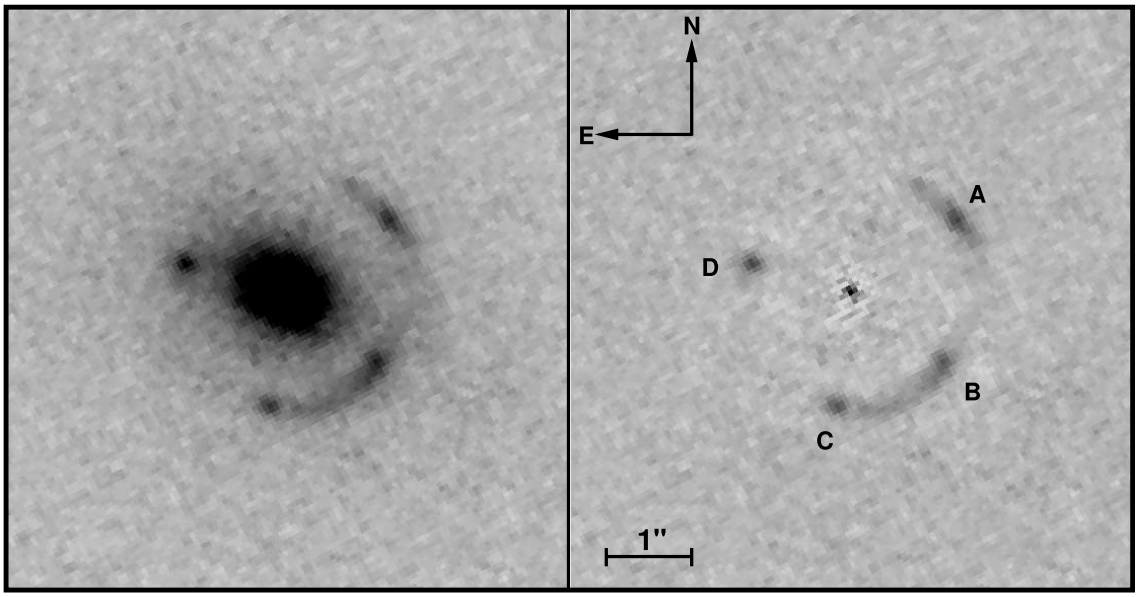
\includegraphics[width=0.95\textwidth]{images/weak_lensing_ellipse/weak_lensing.pdf}
      \caption[Weak Lensing with an Ellipse Galaxy]{
        Galaxy 0047-281 imaged by the Hubble Space Telescope, from Ref. \cite{weak_lensing_ellipse}.
        Left: Original image.
        Right: Same as Left but with the central foreground galaxy subtracted, leaving behind 4 lensed images A, B, C, and D of a background galaxy.
      }
      \label{fig:ellipse}
    \end{figure}
    
    
    Galaxy lensing can be used to estimate the size of the substructure of a lensing galaxy, based on the 4 lensed images of a quasar~\cite{weak_lensing_quasar}.
    The spectra of the four lensed images vary in brightness and distortion.
    These variations can be seen by looking at the ratio of the widths of different spectral lines.
    These ratios of different lensed images indicate that there exists variations in the mass density in the lensing galaxy.
    These variations are best fit by randomly distributing spheres of lensing mass throughout the lensing galaxy, each having a mass of \SI{10^6}{\Msol}.
    This spheres of this mass are consistant with the scale of dark matter substructure predicted by CDM.
    
    


  \subsection{Scales of $10^{23}\:\text{m}$ : Galaxy Clusters}\label{dm_galclusters}
    %
    % galaxy cluster wiki page
    % 2-10 Mpc, call it 6Mpc = 1.85*10^23m ~ 10^23m
    At scales of $\nicetilde 10^{23}$m, dark matter's effects on galactic clusters become observable with several techniques.
    In one technique, the mass-to-light ratio can be measured for galaxy clusters.
    This is done the same as with dwarf galaxies; luminous mass is derived from the brightness of the cluster, while total mass is measured from the velocity dispersion of individual galaxies within the cluster.
    From measurements of several hundred galaxy clusters, it was found that galaxy clusters have mass-to-light ratios of \SIrange{10}{1000}{$\frac{\Msol{}}{\Lsol{}}$}~\cite{cluster_ml_ratios}, indicating a very high amount of dark matter is present in these objects.

    \begin{table}
      \centering
      \caption[Ratios of \MLsol for Various Galaxy Clusters]{Ratios of \MLsol for various galaxy clusters~\cite{cluster_ml_ratios}.}
      \label{tab:cluster_ml_ratios}
      \begin{tabular}{l r | l r | l r}
        Object & \mlratio{} & Object & \mlratio{} & Object & \mlratio{} \\
        \hline
        Abell   85 & 445 & Abell 2426 &  80 & Abell 3695 & 180 \\
        Abell  458 & 401 & Abell 3122 & 960 & Abell 3921 & 175 \\
        Abell  999 & 100 & Abell 3126 & 491 & Abell 4008 & 227 \\
        Abell 1228 &  37 & Abell 3354 &  94 & Abell 4053 & 421 \\
      \end{tabular}
    \end{table}
    
    Another technique for measuring the total mass is by examining the amount of gravitational lensing caused by a cluster.
    When a massive galaxy cluster has a galaxy directly behind it, the image of the background galaxy gets distorted.
    The shape of the distorted image can then be used to infer the amount of total mass in the galaxy cluster.
    Then comparing this total mass to the luminous mass provides an estimate for the amount of dark matter contained in the galaxy cluster.
    This was used with galaxy clusters Abell 370 and CL 2244-02 to estimate the amount of dark matter in each~\cite{cluster_lensing}.
    Lensing cluster Abell 370 and several distorted background galaxies are shown in Figure~\ref{fig:abell370}.
    This technique found that for both Abell 370 and CL 2244-02, a large amount of dark matter is required to fit the observed arcs, within the range of 200-1000 \MLsol.
    
    \begin{figure}
      \centering
      \includegraphics[width=0.95\textwidth]{images/abell370/abell370_cropped.pdf}
      \caption[Gravitational Lensing in Abell 370]{
        Galaxy cluster Abell 370 is shown here, along with many gravitationally lensed background galaxies.
        The large arc marked by the green lines is the distorted background galaxy image used to calculate the cluster's total mass~\cite{cluster_lensing}.
        Credit: NASA, ESA/Hubble, HST Frontier Fields~\cite{abell370_hubble}.
      }
      \label{fig:abell370}
    \end{figure}
    
    Another example of using gravitational lensing to measure dark matter mass is with cluster Cl0024+1654.
    This galaxy cluster creates several lensed images of the same background galaxy, which are used to measure the total mass
    The lensing is shown in Figure~\ref{fig:stronglens}, where the blue arcs are the distorted background galaxy images.
    From all of these lensed images, the best fit amount of dark matter indicates this cluster has a mass-to-light ratio of \SI{161}{}\MLsol{}\footnote[3]{This measurement scales with the hubble constant, which here is assumed to be \SI{70}{km/s/Mpc}}~\cite{cluster_strong_lensing_1996, cluster_strong_lensing_1998, cluster_strong_lensing_2010}.
 %assumes a hubble constant of 70\SI{230}$\,h_{70}\,$\MLsol, where $h_{70}$ is set to $0.70$
    
    \begin{figure}
      \centering
      \includegraphics[width=0.95\textwidth]{images/cluster_strong_lensing_8/stronglensing2.pdf}
      \caption[Gravitational Lensing in Cl0024+1654]{
        Strong lensing of a blue background galaxy by galaxy cluster Cl0024+1654 into multiple blue distorted images~\cite{cluster_strong_lensing_1996}.
      }
      \label{fig:stronglens}
    \end{figure}
    
    Yet another way of measuring the total mass of a cluster is by examining X-ray measurements.
    In galaxy clusters, the majority of the luminous mass is stored in warm ($kT\simeq\,$\SI{5}{keV}) gas, rather than stars.
    This warm gas emits X-rays, which can be detected by satellites like Chandra~\cite{chandra}.
    By measuring the X-ray flux at the center of the galaxy cluster Abell 2029, the total mass of the cluster can be measured.
    This is done by assuming the warm gas is in hydrostatic equilibrium, where the force of gravity towards the cluster center is equally balanced by the pressure of the warm gas.
    This implies that when moving outwards from the cluster center, the density and temperature of the gas is predictable.
    From this, the mass-to-light ratio can be inferred at several different radii from the cluster center.
    Within \SI{28.5}{kpc}\footnote[2]{This scales inversely with the hubble constant, assumed here to be \SI{70}{km/s/Mpc}} of the center, the ratio is 12 \MLsol, while beyond a radius of \SI{286}{kpc}\footnotemark[2] the ratio rises above 100 \MLsol{}, indicating a high amount of dark matter is present~\cite{cluster_chandra}.
    
    These previously mentioned techniques have been combined into an analysis of galaxy cluster 1E 0657-558 to provide a cardinal piece of evidence in favor of particle dark matter.
    Galaxy cluster 1E 0657-558 consists of two subgroups of galaxies, a larger 'target' cluster, and a smaller Bullet cluster.
    Each cluster's mass is contained in two clouds; gas and stars that form the baryonic cloud, and the much more massive dark matter cloud.
    The baryonic cloud is visible through Chandra X-ray observations, which is able to image the warm ($kT\simeq\,$\SI{10}{keV}) gas and infer its density.
    The dark matter cloud is inferred through weak lensing observations, where the mass of the cluster distorts the images of background galaxies.
    In this pair of clusters, the Bullet cluster has fallen through the target cluster.
    However, the two clouds of the Bullet cluster dragged on the clouds of the target cluster, and dragged at different rates.
    This difference in drag over time resulted in a separation between the Bullet cluster's baryonic and dark matter clouds.
    , visible in Figure~\ref{fig:bullet}.

    \begin{figure}[ht]
      \centering
      \includegraphics[width=0.95\textwidth]{images/bulletcluster/bulletcluster_cropped.pdf}
      \caption[The Bullet Cluster]{
        The Bullet Cluster~\cite{bullet_cluster_combined_image}.
        The blue clouds indicate the graviational lensing mass~\cite{bullet_cluster}, the pink represents clouds of warm gas emitting X-rays~\cite{bullet_cluster_chandramap}.
        The red triangle indicates the bullet cluster's warm gas center-of-mass, and the blue oval marks the approximate center of the weak lensing (dark) mass.
        The remaining stars and galaxies are imaged in the optical spectrum~\cite{bullet_cluster_composite}.}
      \label{fig:bullet}
    \end{figure}
    
    The pink clouds are X-ray observations of the cluster's warm gas, while the blue clouds are the weak lensing mass.
    The red triangle and blue oval show the approximate centers of mass of the bullet cluster's two clouds.
    The difference in position between the two centers of mass allows for constraints to be put contraints on the mass and cross section.
    This contraint is shown in Equation~\ref{eqn:bullet}, where $\sigma_{\chi}$ is the dark matter particle cross section, and $m_{\chi}$ is the dark matter particle mass~\cite{bullet_cluster,bullet_cluster2}.
    
    \begin{equation}\label{eqn:bullet}
      \frac{\sigma_{\chi}}{m_{\chi}} < 1 \, \textrm{cm}^2 \, \textrm{g}^{-1}
    \end{equation}
    
    This result was improved by combining 72 galaxy cluster collisions, improving the limit in Equation~\ref{eqn:bullet} to \SI{0.47}{$cm^{2} g^{-1}$}~\cite{cluster_72}.


  \subsection{Scales of $10^{26}\:\text{m}$ : The Observable Universe}\label{dm_universe}
    %\subsection{Inter-Cluster Scale}
    % age of universe (13.82*10^9 years * speed of light) = 1.307*10^26m
    At the universe's largest scale, $\nicetilde 10^{26}$m, the Cosmic Microwave Background (CMB) has been used to measure the total amount of dark matter in the universe.
    By looking at the structure of the CMB, the structure of the universe and its particle populations can be studied, including how they developed and changed from the big bang to the present day.
    In order to understand dark matter's place in the evolution of the universe, several important moments must be discussed.
    The first moment of the universe was Inflation, where a singularity with a temperature of $kT=10^{17}\:\textrm{GeV}$ quickly expanded as a quark-gluon plasma and cooled~\cite{inflation0,inflation1,inflation2,inflation3}.
    Once the average temperature had reduced enough, quarks could bind together to form baryons, in a stage known as Baryogenesis.
    The time/temperature that Baryogenesis occurred at has not been determined.
    However, there are several competing theories that may explain how an unequal ratio of baryons to antibaryons were created~\cite{baryogenesis1,baryogenesis2}.
    
    Later on when the universe is around \nicetilde380,000 years old and has expanded enough to cool to \nicetilde\SI{3000}{K}, another phase change can occur.
    Here, the universe is a sea of photons ($\gamma$) and free electrons and protons.
    With all the free electrons and protons around, the mean free path of the photon is small, so they are in thermal equilibrium with the electrons and protons.
    Once the universe expands further, enough to cool below the electron-proton binding energy, electrons start being captured by protons in great numbers.
    Since electrons and protons have formed electrically neutral hydrogen atoms (an event called recombination), the universe becomes transparent to these photons, which are then free to travel the universe~\cite{planck2015,theEarlyUniverse,CMBFundamentals,CMBFlat}.
    The spectrum of these photons follow a blackbody spectrum, shown in Figure~\ref{fig:cmb_black}, and is called the cosmic microwave background.
    
    \begin{figure}[t]
      \centering
      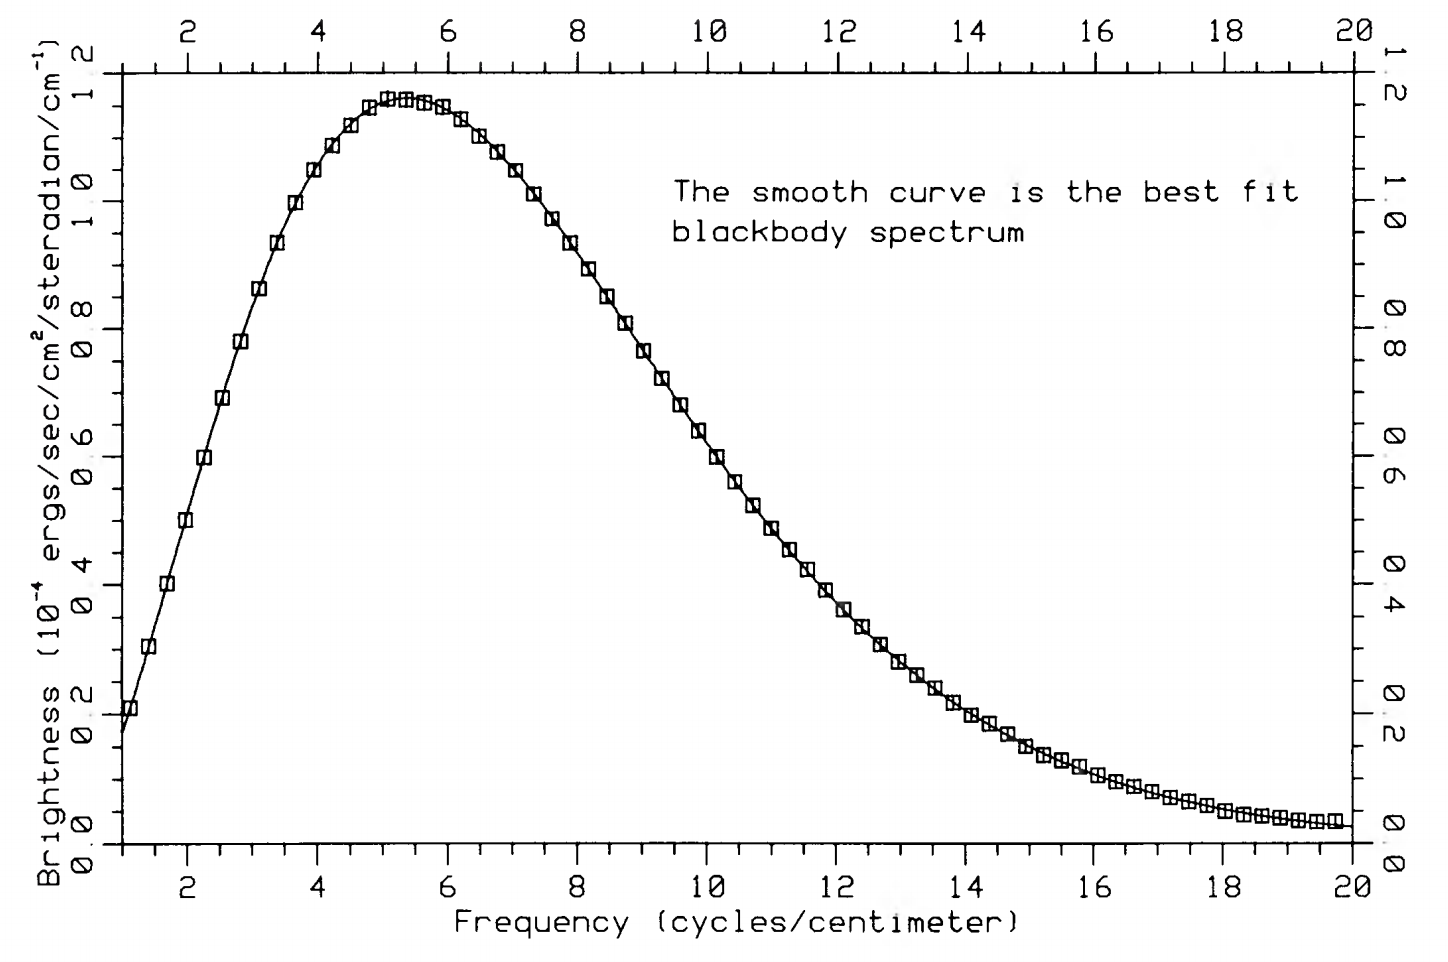
\includegraphics[width=0.85\textwidth]{images/cmb_blackbody/cmb.pdf}
      \caption[Cosmic Microwave Background Blackbody]{
        The blackbody spectrum of the cosmic microwave background measured by the FIRAS instrument on the COBE satellite~\cite{mather1990}.
        Errorbars shown are from an assumed 1\% error.
      }
      \label{fig:cmb_black}
    \end{figure}
    
    However, the CMB spectrum varies a small amount from a pure blackbody spectrum.
    These variations also depend on the region of the sky measured, which is shown in Figure~\ref{fig:cmb}

    \begin{figure}[t]
      \centering
      \includegraphics[width=0.95\textwidth]{images/cmb_skymap/cmb_skymap.eps}
      \caption[Cosmic Microwave Background Skymap]{
        The cosmic microwave background temperature map of the universe \cite{wmap_skymap}, from 9 years of WMAP observations~\cite{wmap9year}.
        This image shows a temperature range of \SI{\pm200}{\mu{}Kelvin}.
      }
      \label{fig:cmb}
    \end{figure}

    These deviations are due to Baryon Acoustic Oscillations (BAOs).
    The recombination of electrons and protons was not an instantaneous event, and instead happend over time.
    During this gradual recombination, some baryons were gravitationally pulled into areas of high mass densities.
    These high-mass areas were formed in earlier times of the universe, and were spread out evenly.
    The baryons would fall into these gravitational wells, until they became warmer, whereupon the baryons emit more photons, which increases the photon pressure and drives the baryons out of the wells.
    Eventually after leaving the wells, the photon pressure decreases and the gravitiational force takes over, drawing the matter back towards the gravitational wells again.
    After happening repeatedly, this created ripples of density waves (acoustic oscillations), which spread outwards, interferring with one another.
    These density waves, which had dense high-temperature areas, and sparse low-temperature areas, then emitted blackbody photons at higher and lower temperatures, respectively.
    These higher and lower temperatures account for the spectrum of variations in the CMB's temperature in different parts of the sky.
    
    As the CMB is emitted by scattering off the baryons, the CMB spectrum only depends on the baryon temperature.
    However, since the baryons were pulled into the high density areas by gravity, the presence of dark matter increases the wavelength of these density ripples.
    This is similar to a simple spring pendulum, where adding an extra (dark) mass to an existing (baryonic) mass will decrease the oscillation frequency ($\omega = \sqrt{\frac{k}{m}}$), resulting in BAOs with longer wavelengths.
    Thus, by measuring the wavelength of the BAOs with the CMB correlations, the amount of dark matter in the universe can be measured.
    The CMB correlation spectrum, measured by Planck, is shown in Figure~\ref{fig:cmb_correlation_spectra}.
    
    \begin{figure}[t]
      \centering
      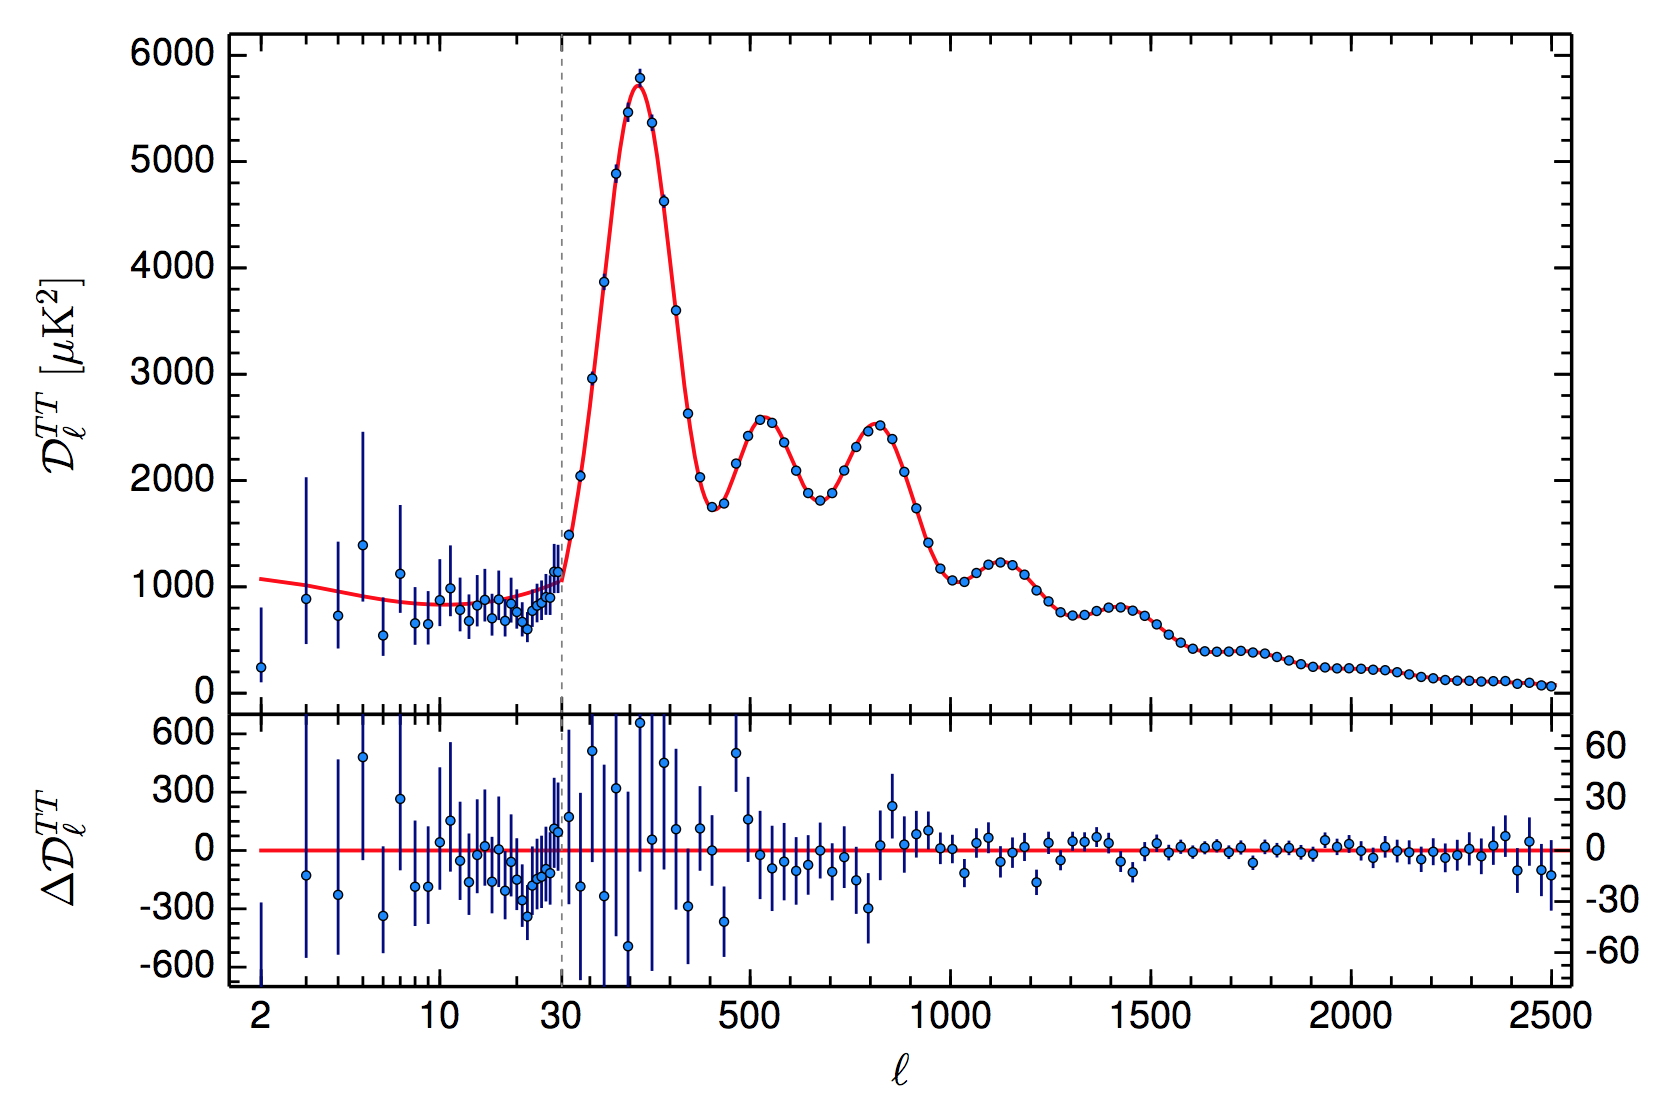
\includegraphics[width=0.85\textwidth]{images/cmb_spectra_planck_2018/cmb_spectra.pdf}
      \caption[Cosmic Micrwave Background Correlation Spectrum]{
        Correlation spectra from CMB temperature measurements with the Planck satellite~\cite{planck_dm_limit}.
        The upper plot shows the spectra, the lower panel shows the residuals.
      }
      \label{fig:cmb_correlation_spectra}
    \end{figure}
    
    From the BAOs in Figure~\ref{fig:cmb_correlation_spectra}, it has been found that 68.6\% of the universe is stored in Dark Energy, a repulsive force which causes almost all visible galaxies to accelerate away from the Milky Way.
    % 100% - ( 26.5% + 4.9 ) = 73.5% (from beginning of chapter)
    Another 4.9\% of the universe's energy is stored in baryonic matter, like protons and neutrons.
    The remaining 26.5\% of the universe's energy is contained in dark matter~\cite{planck2015}.
    
    The polarization of CMB photons also incorporates information about dark matter and its properties.
    The CMB photons come from ambient photons that Thompson-scattered off electrons right before recombination.
    Because of this Thompson scattering, the CMB photons inherit both temperature and polarization information.
    Dark matter annihilations during recombination may produce standard model particles, which act as an injection of ionization energy, which extends the duration of recombination.
    A longer recombination acts to decrease any CMB temperature fluctuations while increasing CMB polarization fluctions~\cite{cmb_polarization1,cmb_polarization2}.
    
    The observed quantities of deuterium in the early universe also hint at dark matter's properties.
    During Big Bang Nucleosynthesis when the universe was only a few seconds old, protons and neutrons were starting to combine into various isotopes, one of which is deuterium.
    However, like baryons, the amount of deuterium produced in the early universe is heavily dependent on the initial baryon number density.
    So, any constraint on the deuterium fraction is also a constraint on the baryon fraction of the universe~\cite{deuterium1,deuterium2}.
    From the spectrum of deuterium and hydrogen lines from the quasar QSO Q0913+072, the baryon fraction was measured to be $\Omega_{b}h^2 = 0.0224 \pm 0.0005$~\cite{deuterium3}, indicating only 4.93\% of the universe's energy is stored in baryons.
    % h = 0.674 (see below)
    % 0.0224 / h^2 = 0.0224 / 0.674^2 = 0.0493 -> 4.93% of universe's energy
    This then suggests that the majority of matter in the universe cannot be made of baryons, and that the majority resides in some non-baryonic form.
    
    Another measurement that depends heavily on the presence of dark matter is the rate at which galaxies cluster together.
    In the Sloan Digital Sky Survey (SDSS), the positions of 1.6 million galaxies, quasars, and stars are mapped~\cite{sdss_release}.
    By simulating the distribution of similar objects as the universe ages, only with extra mass from dark matter does the universe form clumps that match SDSS observations.
    
    

\section{$\Lambda$CDM Cosmology and the Standard Model}

  The measurements of the CMB (discussed in Section~\ref{dm_universe}) contribute to the existing theory of how the universe developed after the big bang, called $\Lambda$CDM.
  The $\Lambda$ refers to the density of dark energy, while CDM refers to Cold Dark Matter.
  This theory predicts the different times particles froze out of the universe, and their resulting distributions.
  From the CMB correlation spectrum in Figure~\ref{fig:cmb_correlation_spectra}, six parameters that describe the universe can be modelled~\cite{planck_dm_limit,planck_2013_parameters}.

  % from planc 2018 results cosmological constants, table 1
  % hubble constant :
  %   H_0 = (67.4+-0.5) km/s/Mpc
  %   h = H_0 / 100 km/s/Mpc = 0.674
  % \Omega_b h^2 = 0.02233 +- 0.00015
  %   \Omega_b = 0.02233 / h^2 = 0.02233 / 0.674^2 = 0.04915 -> 4.915 +- 0.033 %
  % \Omega_c h^2 = 0.1198 +- 0.0012
  %   \Omega_c = 0.1198  / h^2 = 0.1198  / 0.674^2 = 0.2637  -> 26.37 +- 0.264 %
  % ln( A_s * 10^10 ) = 3.043 +- 0.014
  %   A_s = e^(3.043+-0.014) * 10^-10 = (2.097+-0.029)*10^-9
  %   
  
  \begin{table}[b]
    \centering
    \caption[6 Cosmological Parameters]{
      The best fit values for the six cosmological parameters using CMB measurements, from Ref.~\cite{planck_dm_limit}}
    \label{tab:six_params}
    \begin{tabular}{llcl}
               & \textbf{Value}                 & \textbf{Unit} & \textbf{Description} \\
    \hline 
    $\Omega_b$ & $ 4.915  \pm0.033                 $ & \%       & Universe's energy in Baryons \\
    $\Omega_c$ & $ 26.37  \pm0.264                 $ & \%       & Universe's energy in Dark Matter \\
    $\thetamc$ & $(1.04089\pm0.00031)\times 10^{-2}$ & Radians  & Angular size of the sound horizon \\
    $\tau$     & $(5.40   \pm0.74   )\times 10^{-2}$ & unitless & Thompson scattering optical depth (opacity)\\
    % arxiv: 0205436 , section II, 3rd paragraph
    $A_s$      & $(2.097  \pm0.029  )\times 10^{-9}$ & unitless & Seed density spectrum amplitude \\
    $n_s$      & $ 0.9652 \pm0.0042                $ & unitless & Seed density spectrum spectral index \\
    \hline 
    \end{tabular}
  \end{table}
  
  These are shown in Table~\ref{tab:six_params}.
  The parameters $\Omega_b$ and $\Omega_c$ are the fraction of the universe's energy stored in baryons and cold dark matter, respectively.
  The parameter $\thetamc$ is the angular range that could be influenced during the BAOs produced after recombination.
  This is the comoving distance a sound wave could have traveled between the beginning of the universe and recombination.
  The parameter $\tau$ describes how opaque the universe became to photons during reionization, where the first stars started to reheat atoms and free electrons.
  The parameters $A_s$ and $n_s$ govern the amplitude and the spectral index of the initial seed perturbations in the early universe.
  These universe-scale parameters determine how the universe evolved over time.
  However, dark matter is likely a new, undiscovered particle,  so a discussion of particle physics is necessary to understand what particle properties it may possess.
  

  The current paradigm of particle physics is called the Standard Model~\cite{standardmodel}.
  It consists of groups of particles called quarks and leptons, as well as the bosons that mediate interactions between these particles.
  Quarks combine to form hadrons, like protons and neutrons, and mesons, while leptons consist of electrons, muons, tauons, and their neutrino companions.

  At the forefront of dark matter search candidates are particles predicted by Supersymmetry~\cite{Jungman:1995df}, (specifically Minimal Supersymmetric Standard Model, or MSSM~\cite{MSSM,supersym1}), an extension to the Standard model.
  Much like how most particles have an anti-particle, in supersymmetry, each Standard Model quark, lepton, and boson has a supersymmetric partner particle.
  Quarks and leptons have squarks and sleptons as their supersymmetric partners, while bosons have partners like photinos, gluinos, and charginos.
  While no evidence of supersymmetry has been discovered to date, it is still preferred due to its ability to predict physics across a large range energy scales, the holy grail of any Grand Unified Theory.
  

\section{Particle Dark Matter}\label{sec_particledm}

  Early in the search for a candidate dark matter particle, Standard Model (SM) particles were first considered.
  One dark matter candidate was the neutrino, due to how many there are in the universe and their lack of interaction with the strong and electromagnetic forces.
  This was generally referred to as Hot Dark Matter, as neutrinos travel at relativistic speeds.
  However, it was eventually demonstrated that because of these relativistic speeds, neutrinos would diffuse out of their initial overdensities.
  This would result in large super-cluster-scale gravitational wells forming first, then cluster-scale wells, then galaxy-scale wells, called top-down structure formation.
  When observations are made of earlier times, the opposite is found: galaxy-scale gravitational wells form first, then cluster-scale wells, then super-cluster-scale wells in present times, called bottom-up formation.
  As this is the opposite of what is expected for relativistic dark matter, neutrinos were ruled out as a dark matter candidate~\cite{neutrinoHeirarchical}.
  % from this discussion: https://physics.stackexchange.com/questions/158319/why-are-neutrinos-ruled-out-as-a-major-or-even-sole-component-of-dark-matter
  In addition, limits on the mass of the neutrino ($\sum{}m_{\nu} = 0.194 \; \textrm{eV}, \; 95\% \; \textrm{C.L.}$) also rule it out since they are not numerous enough~\cite{planck2015}.
  % see table 5, sum m_nu [eV] row, TT, TE, EE+lensing+ext column
  All other Standard Model particles have also been ruled out, usually for reasons of charge, mass, number density, or cross section.
  Since none of the Standard Model particles meet the conditions to be a dark matter candidate, theoretically predicted particles are now the focus of most searches.
  
  One of the major expansions to the Standard Model that may contain a dark matter candidate is Supersymmetry, or SUSY.
  There are several SUSY extensions, but the main one discussed here is the Minimal Supersymmetric Standard Model (MSSM)~\cite{MSSM,supersym1,schelke_thesis}.
  The basic idea of SUSY is that, just as majorana fermions have a particle-antiparticle reflection, SUSY adds another reflection called R-parity for all particles. 
  This R-parity is defined as

  \begin{equation}
    R = (-1)^{3B+L+2S}
  \end{equation}

  where $B$ is the baryon number, $L$ is the lepton number, and $S$ is the particle spin.
  This creates supersymmetric partner particles (superpartners) for each Standard Model particle, usually denoted by an 's-' prefix or an '-ino' suffix added to a particle name, and \nicetilde{} added atop the particle symbol ($e \rightarrow \tilde{e}$).
  Quarks become squarks, leptons become sleptions, gluons become gluinos.
  Standard model particles and fields have an R-parity of +1, while superpartners have an R-parity of -1.
    
  When this SUSY reflection is performed, the superpartners develop some interesting properties.
  The superpartners all have their spin reduced by $\frac{1}{2}$, so the fermionic electron with spin $\frac{1}{2}$ becomes a bosonic selectron with spin $0$, and the bosonic photon with spin 1 becomes the fermionic photino with spin $\frac{1}{2}$.
  When several of the bosons are reflected, a new set of 4 particles called neutralinos may form.
  These neutralinos are made of the Bino, the Wino, and the two Higgsino fields.
  The Bino is the superpartner of the weak hypercharge, the Wino is the superpartner of the weak bosons, and the two Higgsino fields are superpartners to the Higgs field.
  The lightest of these neutralinos has some properties that make it an excellent dark matter candidate, and is the WIMP candidate searched for in this thesis.
  Specifically, as it is the lightest neutralino, other neutralinos will decay into it.
  If R-parity is conserved, then this neutralino will also be stable, and not decay into anything else~\cite{neutralino1,neutralino2,neutralino3}.
  These two features would give the neutralino the stability and numbers needed to match predictions from dark matter observations.
  
  \subsection{Relic Freezeout and WIMP Miracle}
  
  %This means it would be able to exist since the freezeout without significant losses to its population
  The relic freezeout refers how dark matter may have behaved in the past.
  A population of dark matter particles existed during the early universe (a relic particle), and that at a later time the universe expanded enough that their numbers stopped changing (the freezeout).
  
  This freezeout is relevant because it hints at the self-interacting cross section of the WIMP.
  Early on when the universe was still expanding, its been theorized that WIMPs were annihilating into SM particles, and SM particles were interacting and producing WIMPs.
  The number density and cross section of these two particle populations were such that that the number of WIMPs and SM particles remained constant; the two particle populations were in thermal equilibrium.
  
  As the universe expanded, both particle groups ran into each other less and less.
  This meant that fewer particles were converted to the opposite population, meaning temperature changes in one population took longer and longer to propagate to the other population.
  Eventually the two populations became independent, sometimes called thermal decoupling.
  After this decoupling, WIMPs continued to annihilate occasionally, further reducing their numbers, until there were so few left that they stopped encountering each other.
  As the population of WIMPs likely did not change much after that time, it is called a freezeout.
  
  The boltzman equation describing how the number of WIMPs evolves through this freezeout is,
  
  % some of this derivation is from https://ned.ipac.caltech.edu/level5/March10/Garrett/Garrett7.html
  %   for example, this is equation 20:
  \begin{equation}\label{eqn:boltzmann_relic}
    \frac{dn}{dt} = - 3 H n \: - \left \langle \sigma_{A} v \right \rangle \left ( n^2 - n_{eq}^2 \right ) \;\;,
  \end{equation}
  
  where $n$ is the comoving WIMP number density, $H$ is the hubble expansion rate ($\frac{\dot{a}}{a}$), $\left \langle \sigma_{A} v \right \rangle$ is the velocity-averaged cross section for $\chi\chi$ annihliating into lighter particles~\cite{wells_relic}.
  The parameter $n_{eq}$ is the equilibrium WIMP comoving number density.
  This equation is numerically solved and shown in Figure~\ref{fig:abundance}.
  
  \begin{figure}[ht]
    \centering
    \includegraphics[width=0.75\textwidth]{images/relic_abundance_plot/updated.pdf}
    \caption[Relic Abundance vs Time]{
      The relic abundance of WIMPs as a function of temperature, from Ref.~\cite{updatedWIMPRelicCrossSection}.
      $m$ is the WIMP mass, $T$ is the universe's temperature, which decreases as the universe expands.
      $x$ is therefore a proxy for time, increasing as one moves to the right along the x-axis.
      $n(x)$ is the number of WIMPs in a comoving volume, $n_{\textrm{eq}}(x)$ is the number of WIMPs at equilibrium, and the y values are scaled by $n_{\textrm{eq}}(x=1)$.
      The weak, electromagnetic (em), and strong cross sections are shown for a \SI{100}{GeV} WIMP, with additional lines for the weak cross section at \SI{1}{GeV} and \SI{e3}{GeV}.
      The cross sections shown are:
      \begin{tabular}{ll}
      $\left \langle \sigma v \right \rangle_{\textrm{weak}}  $  & $= 2 \times 10^{-26} \; \textrm{cm}^3 \textrm{s}^{-1}$ \\
      $\left \langle \sigma v \right \rangle_{\textrm{em}}    $  & $= 2 \times 10^{-21} \; \textrm{cm}^3 \textrm{s}^{-1}$ \\
      $\left \langle \sigma v \right \rangle_{\textrm{strong}}$  & $= 2 \times 10^{-15} \; \textrm{cm}^3 \textrm{s}^{-1}$ \\
      \end{tabular} .
    }
    \label{fig:abundance}
  \end{figure}
  
  In this figure, it can be seen how the number of WIMPs evolve as the universe ages, and its temperature decreases.
  The black equilibrium line indicates the number of WIMPs that would be left if they had a large ($\left \langle \sigma v \right \rangle >> 2 \times 10^{-15} \textrm{cm}^3 \textrm{s}^-1$) cross section.
  As the cross section decreases, fewer and fewer particles are annihilated, and more of the initial WIMP population survives to freeze out.
  This freezeout can be thought of as the universe expanding faster than the particles can annihilate.
    
  Weak force cross section
  

  Wimp miracle

  Heavier WIMPs are sought in this thesis, with a mass \SIrange{4}{70}{TeV}.
  At these masses, the WIMP relic cross section is \nicetilde\SI{2.3e-26}{cm^3 s^{-1}}, and not very dependent on mass~\cite{updatedWIMPRelicCrossSection}.
  % 2.3e-26 is from Steigman 2012, Figure 5, measuring the value at 4 TeV



  




  %The cross section of the WIMP heavily influences the time of the freezeout, as well as the final number density.
  
  %This neutralino would also have a cross section of around \nicetilde{} \SI{3e-26}{ cm${}^2$ }~\cite{Jungman:1995df} {\color{red}(verify this is actually in Jungman 1995??)}.
  
  %WIMP Miracle
  
  %"Exact Cross Sections for the Neutralino WIMP Pair-Annihilation" : arxiv 0202009
  %Steigman 2012 Precise relic WIMP abundance : https://journals.aps.org/prd/abstract/10.1103/PhysRevD.86.023506
  

  % Perkins 2003, section 7.11 is a good source
  %Any dark matter candidate particle that meets the cosomological and particle conditions is called a WIMP, or Weakly Interacting Massive Particle.
  %A currently favored WIMP candidate is the neutralino, the lightest supersymmetric particle (LSP)~\cite{neutralino1,neutralino2,neutralino3}.

    % see http://www.damtp.cam.ac.uk/user/db275/Cosmology/Lectures.pdf section 3.3.2
    %After this inflationary period, another important epoch was the WIMP freeze-out, when the universe was roughly 1 second old, though this time can vary by several orders of magnitude..
    %At this point, it is theorized that a population of WIMP dark matter particles were being repeatedly created and annihilated, and were in equilibrium.
    %After the universe expanded some more, the density of these WIMPs decreased to the point where they were no longer running into each other.
    %This increased WIMP transparency froze the number of WIMPs at that time, called the relic density.
    %From the Boltzman Equation~\ref{eqn:boltz_dm}, a relationship can be estabilshed between the WIMP mass, cross section, and how many WIMPs are left over, frozen out (the relic density).
    
    % from http://www.damtp.cam.ac.uk/user/db275/Cosmology/Lectures.pdf
    %\begin{equation}\label{eqn:boltz_dm}
      %\frac{dN_\chi}{dt} = -s \left \langle \sigma v \right \rangle \left [ N_\chi^2 - \left ( N_\chi^{eq} \right )^2 \right ]
    %\end{equation}
    
    %where $N_\chi$ is the number of WIMPs in a comoving volume, $N_\chi^{eq}$ is the number of WIMPs at equilibrium, $s$ is the Friedmann-Robertson-Walker metric, and $\left \langle \sigma v \right \rangle$ is the velocity-averaged cross section of the WIMP annihilation.
    %After many substitutions and some assumptions\footnote{This derivation is explained more thoroughly in \url{http://www.damtp.cam.ac.uk/user/db275/Cosmology/Lectures.pdf}}, one finds that for a \nicetilde{}GeV WIMP and the observed relic abundance, the WIMP must have a $\left \langle \sigma v \right \rangle$ close to the Weak force cross section for a \nicetilde{}GeV particle.
    %This coincidence between the dark matter abundance and the particle physics cross section is sometimes called \textit{WIMP Miracle}.
    
    % see http://pdg.lbl.gov/2013/reviews/rpp2013-rev-dark-matter.pdf for more basic info
    % see https://arxiv.org/pdf/1603.03797.pdf
  
  
  % Hypercharge :
  %   Y = ( B + S + C + B' + T)
  %     B  : baryon number
  %     S  : strangeness
  %     C  : charm-ness
  %     B' : bottomness
  %     T  : topness
  %   proton : +1
  %   strong interactions conserve hypercharge,
  %     weak interactions do not
  %
  % Weak Hypercharge :
  %   Y_W = 2(Q-T_3)
  %     Q   : electric charge
  %     T_3 : third component of weak isospin (the SU(2) component)
  %   For several particles
  %     leptons : -1
  %     quarks  : +1/3
  %     W+-,Z   : 0
  %     Higgs   : +1
  
  % Minimal Supersymmetric Standard Model
  % New features:
  %   R-parity,  P_R = (-1)^{3B+L+2s}
  %     B : baryon number
  %     L : lepton number
  %     s : spin
  %     Standard model particles have P_R = +1
  %     Supersymmetric partners  have P_R = -1
  %     e.g. 
  %       electron has L=1, s=1/2, so P_R = (-1)^{3*0+1+2*1/2} = (-1)^2 = +1
  %       baryon has B=1, s=1/2  , so P_R = (-1)^{3*1+0+2*1/2} = (-1)^4 = +1
  %     If R-parity is preserved, the lightest supersymmetric particle can't decay,
  %       making it a good candidate for dark matter
  %   New Particles:
  %     Rules:
  %       Supersymmetric partner particles subtract 1/2 from spins:
  %         fermions : (spin 1/2) -> sfermions (spin 0  )
  %         bosons   : (spin 1  ) -> bosinos   (spin 1/2)
  %     +2x Higgsino fields
  %       dsb couple to higgs field, uct couple to higg's complex conjugate
  %         this is not allowed in SUSY, so therefore two higgino fields are needed
  %     +Squarks
  %       superpartners to quarks
  %       3 flavors (sup,scharm,stop,etc)
  %     +Sleptons
  %       superpartner to leptons
  %     +Charginos
  %       fermions, electrically charged
  %     +Gluinos
  %       superpartner to gluon
  %     +Neutralinos
  %       4 different ones
  %         lightest is usually stable
  %         made from mixtures of:
  %           Bino, gauge field corresponsing to the weak hypercharge
  %           Winos, superpartner to W+-0 bosons
  %           2x Higgsinos (can't have just one higgsino in SUSY)
  %       fermions (majorana, so each is its own anti-particle)
  %       electrically neutral
       
  
  %The standard model has a set of gauge and higgs fields $\left \{ B,W_3,H_1,H_2 \right \}$.
  %$B$ is the photon, $W_3$ is the weak gauge bosons $W^{\pm}$ and $Z^0$, and $H_1$ and $H_2$ are two higgs fields.
  %In supersymmetry, this set has a supersymmetric partner set ${\chi_1,\chi_2,\chi_3,\chi_4}$.
  %The neutralino is $\chi_1$, the lightest of these partner particles.
  %The neutralino is a good candidate as a dark matter particle because it is neutral in charge and color, and being the LSP, all other supersymmetric particles eventually decay/annihilate into the LSP, providing a large population of neutralinos.
  %{\color{red}(why neutralino?, what are its properties?)}
  %One of the major predictions from particle physics and cosmology is referred to as the "WIMP Miracle".
  %In it, particle physics and cosmology separately predict that if dark matter is WIMP, it should have a velocity-averaged cross section of around \SI{ 3e-26 }{ cm$ {}^3 $s$ {}^{-1} $ }, though each field comes to this value by very separate math. {\color{red}(cite?)}
  %{\color{red}(It's not exactly math, there is some physical constraints in it. Can you find a better way of explaining it? -Orel)}

%  Supersymmetry predicts the existance of a WIMP-like particle with a cross section of around \nicetilde{} \SI{3e-26}{ cm${}^2$ }~\cite{Jungman:1995df}.
%  % $3*{10}^{-26}\ {\textrm{cm}}^{2}$
%  What made this WIMP particle a more promising candidate is that several cosmological problems can also be solved by a weakly-interacting GeV-TeV mass particle.
%  {\color{red}What were these cosmological problems that were fixed?}
%  Thus, two separate fields of physics recognized that they both were looking for a WIMP-like particle within the same mass and cross section range.

%  In $\Delta$CDM cosmology, the relic density is all of the leftover dark matter particles after the universe became too cold to produce more dark matter particles.

%  {\color{red}One or two more sentences on the relic density?}
%  % see http://www.damtp.cam.ac.uk/user/db275/Cosmology/Lectures.pdf

%  There are other potential dark matter candidates, both as other particle types or as modifications to other areas of physics, but they are not explored in this thesis.
%  See Ref. \cite{DMPrimer} for more a more detailed discussion.

%  % neutralino as a WIMP: https://arxiv.org/pdf/1707.06277.pdf



\cleartooddpage[\thispagestyle{empty}]


\newcommand{\Lim}[1]{\raisebox{0.5ex}{\scalebox{0.8}{$\displaystyle \lim_{#1}\;$}}}
\renewcommand{\labelitemi}{\textbullet}
\newcommand{\pip}[1]{$\pi^{+}$}
\newcommand{\pim}[1]{$\pi^{-}$}
\newcommand{\pio}[1]{$\pi^{0}$}
\newcommand{\sv}{\left < \sigma v \right >}

\chapter{Gamma Rays and Dark Matter}\label{ch_gamma}


This thesis searches for evidence of dark matter within gamma ray data, but the relationship between these two areas of physics is intricate.
In this chapter three topics relevant to this relationship are discussed.
The first is the astrophysical mechanisms that can produce TeV-energy gamma rays, a background for detecting dark matter gamma rays.
The second is how dark matter around the Galactic Center can produce gamma rays.
The third topic is how gamma rays induce air showers in the Earth's atmosphere.

\section{Production of TeV Gamma Rays}

  There are several mechanisms that can produce photons with TeV energies.
  A gamma ray can start as a low-energy photon, then gain significant energy from electroweak interactions with electrons, referred to as a leptonic production.
  Alternately, a gamma ray can be created from a high-energy proton colliding with another proton, which produces neutral pions ($\pi^0$'s) that decay into gamma rays.
  This is referred to as hadronic production.
  However, leptonic and hadronic production are separate from how gamma rays are produced by dark matter.
  Instead, two WIMP dark matter particles may annihilate (directly or indirectly) into gamma rays, and this is discussed in Section~\ref{dm_spectral}.

  In leptonic production, electrons and low-energy photons collide, transferring energy to the photon.
  This interaction is called inverse Compton scattering (or occasionally upscattering)~\cite{compton_effect}, and its Feynman diagram is shown in Figure~\ref{fig:inv_compt_feyn}.
  
  \begin{figure}[!ht]
    \centering
    \includegraphics[width=0.45\textwidth]{images/feynman_particles/inversecompton.pdf}
    \caption[Inverse Compton Scattering Feynman Diagram]{
      Feynman diagram of inverse Compton scattering, where an electron upscatters a low-energy photon (red) to produce a higher-energy (blue) photon.
    }
    \label{fig:inv_compt_feyn}
  \end{figure}
  \FloatBarrier
  
  In inverse Compton scattering~\cite{inv_compt1,inv_compt2}, a field of photons with an electron present will gain energy according to 
  
  % https://eud.gsfc.nasa.gov/Volker.Beckmann/school/download/Longair_Radiation3.pdf equation 11
  \begin{equation}\label{eqn:inv_compt_en_gain_rate}
    \frac{dE}{dt} = \frac{4}{3} \: \sigma_{t} \: U \: c \: \gamma^2 \: \frac{ v^2 }{ c^2 } \;\; ,
  \end{equation}
  where
  
  \begin{itemize}
    \item $\sigma_{t}$ is the Thomson cross section, $\frac{8\pi}{3} \left ( \frac{\alpha \hbar c}{m c^2} \right )$,
    % Thomson cross section is from wikipedia.org/wiki/Thomson_scattering
    \item $c$ is the speed of light in vacuum,
    \item $\gamma$ is the Lorentz factor,
    \item $U$ is the energy density of the photon field in the rest frame of the electron (e.g. $Uc=N\hbar \omega c$), and 
    \item $v$ is the velocity of the electron in the laboratory frame.
  \end{itemize}
  The average energy $E_{up}$ of photons upscattered this way can be calculated via
  
  % https://eud.gsfc.nasa.gov/Volker.Beckmann/school/download/Longair_Radiation3.pdf equation 15
  \begin{equation}\label{eqn:inv_compt_avg_up_en}
    E_{up} = \frac{4}{3} \: \gamma^2 \: E_{0} \,,
  \end{equation}
  where the parameter $E_{0}$ is the energy of the original photon.
  
  % me = 5e5 eV (mass of electron)
  
  % formula for calculating gamma (lorentz factor) from relativistic kinetic energy
  % Ek = mc^2 / sqrt(1-v^2/c^2) - mc^2
  % Ek + mc^2 = mc^2 / sqrt(1-v^2/c^2)
  % ( Ek + mc^2 ) / mc^2 = 1 / sqrt(1-(v^2/c^2)) = g
  
  % lorentz factor for various kinetic energy electrons
  % Ek = 5e5  eV, 500 KeV, g =   2
  % Ek = 1e6  eV,   1 MeV, g =   3
  % Ek = 1e7  eV,  10 MeV, g =  21
  % Ek = 1e8  eV, 100 MeV, g = 201
  % Ek = 1e9  eV,   1 GeV, g = 2e3
  % Ek = 1e10 eV,  10 GeV, g = 2e4
  % Ek = 5e11 eV, 500 GeV, g = 1e6
  
  % calculating the energy in eV of a green photon
  % lg = 550e-9 m  = 5.5e-7 m
  % c = l*w
  % wg = c / lg
  % wg = 2.99e8 m/s / 5.5e-7 m = 5.4e14 1/s
  % E  = hbar w
  % hbar = 1.05e-34 m^2 kg / s (reduced planck constant)
  % 1 J = 6.24e18 eV
  % Eg = hbar wg
  % Eg = 1.05e-34 m^2 kg / s    * 5.4e14 1/s * 6.24e18 eV/J
  % Eg = 1.05 * 5.4 * 6.24 e-34 e14 e18 eV
  % Eg = 35.3e-2 eV
  % Eg = 0.35 eV (energy of a green photon)
  
  % 500 GeV electron upscatters a 0.35 eV photon (green) into a ? eV photon?
  % gamma = (Ek + Ee) / Ee
  % gamma = ( 5e11 eV + 5e5 eV ) / 5e5 eV
  % gamma = 1e6
  % Eup = (4/3) * gamma^2 * Eg
  % Eup = (4/3) * 1e12 * 0.35 eV
  % Eup = 4.67e11 eV = 467 GeV
  
  Astrophysical electrons have been detected at Earth at energies of \SI{500}{\GeV{}}~\cite{500GeVElectrons,fermi_electron}, and potentially as high as \SI{20}{\TeV{}}~\cite{hess2017_electronspectrum}.
  At energies of \SI{500}{\GeV{}}, the Lorentz factor is $\gamma = 10^6$.
  With this Lorentz factor, upscattered photons can increase their energy by up to\footnote{This is the maximum average energy gain when the upscattered photon is emitted back along its original trajectory.} $\gamma^{2} = 10^{12}$.
  For example, a green photon ($\lambda_{\textrm{green}}=550\,\textrm{nm}$, $E_{\textrm{green}}=0.3\,\textrm{eV}$) could be upscattered to as high as \SI{467}{\GeV{}}, becoming a gamma ray detectable by VERITAS.
  
  In order to efficiently produce gamma rays via this method, a population of high-energy electrons is needed.
  One environment that produces these electrons is pulsar wind nebulae.
  Because pulsars spin rapidly, they produce strong magnetic fields.
  For example, the pulsar at the heart of the Crab nebula has a surface magnetic field strength of \SI{e12}{G}~\cite{pwn_evolution}, much larger than Earth's $\sim$\SI{0.5}{G}~\cite{earth_geomag}.
  These strong magnetic fields provide an environment for producing and accelerating charged particles.
  In these strong magnetic fields, ambient photons can convert into $e^{+}e^{-}$~\cite{pwn_pairprod2,pwn_pairprod3}.
  The probability $\Upsilon$ (0-1) of a photon pair-converting in a magnetic field is calculated by via 
  
  \begin{equation}\label{eqn:pwn_pairprod}
    \Upsilon = \frac{E}{mc^2} \frac{H}{c} \frac{e \hbar}{m^2c^2} \,,
  \end{equation}
  where $E$ is the photon energy, $H$ is the ambient magnetic field strength, $e$ is the electron charge, and $m$ is the mass of the electron~\cite{pwn_pairprod3}.
  The factor $\frac{e \hbar}{m^2c^2}$ acts as a threshold magnetic field strength, above which the conversion rate becomes significant.
  For electrons the threshold is $\frac{1}{4.4\times10^{13}\,\textrm{Gauss}}$, similar in scale to the pulsar's surface magnetic field strength.
  %
  % paper : https://journals.aps.org/rmp/pdf/10.1103/RevModPhys.38.626
  % High-Energy Electromagnetic Conversion Processes in Intesnse Magnetic Fields, T. Erber, 1966
  %    NOTICE: This paper has a mistake in equations 1.1 and 1.1a (a 'c' in 1.1a should be moved to 1.1, thats all)
  %
  % e = 1.602e-19 C
  % hbar = 1.05e-34 J*s
  % m_electron = 9.11e-31 kg
  % c = 2.98e8 m/s
  % 1 Gauss = 1e-4 kg/ A*s^2 = 1e-4 kg C^-1 s^-1
  % 
  % factor = e hbar / m^2 c^2
  %        = 1.602e-19 C * 1.05e-34 J*s / (9.11e-31 kg)^2 (2.98e8 m/s)^2
  %        = 4.4e13 G
  
  Charged particles can also be accelerated by a pulsar's magnetic fields, in a process called magnetic reconnection, shown in Figure~\ref{fig:magcon}.
  In this mechanism, two oppositely oriented magnetic fields move towards each other (Figure~\ref{fig:magcon}.a), due to the field lines being frozen into the local plasma.
  As the magnetic field lines merge (Figures \ref{fig:magcon}.b and c), induced current flows produce electric fields (Figure~\ref{fig:magcon}.d) that can accelerate charged particles~\cite{magcon_crab,magcon_schopper,magcon_review,gamma_pwn1,gamma_pwn2,magconsim2011,magconsim2014,magcon_particleaccel}.
  
  \begin{figure}[!t]
    \centering
    \begin{tabular}{m{1cm}m{10cm}}
      (a) & \includegraphics[width=0.5\textwidth]{images/magnetic_reconnection/diagram_1_cr.pdf} \\
      (b) & \includegraphics[width=0.5\textwidth]{images/magnetic_reconnection/diagram_2_cr.pdf} \\
      (c) & \includegraphics[width=0.5\textwidth]{images/magnetic_reconnection/diagram_3_cr.pdf} \\
      (d) & 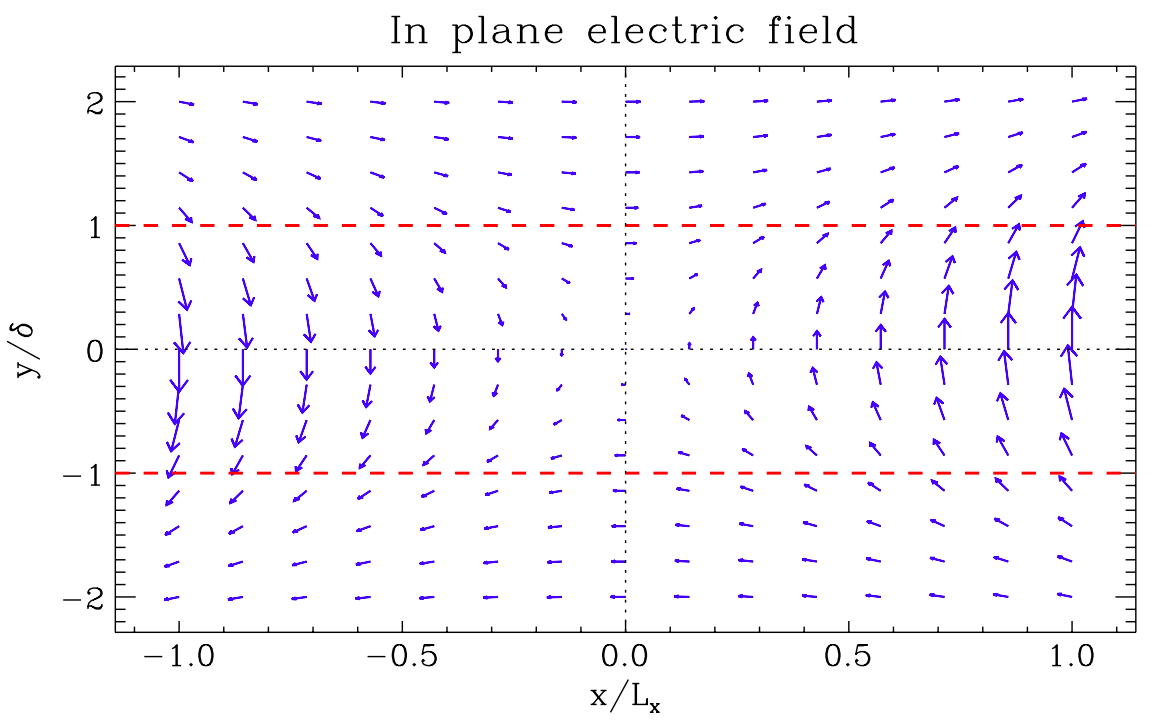
\includegraphics[width=0.5\textwidth]{images/magnetic_reconnection/magcon_efieldlines.pdf}
    \end{tabular}
    \caption[Magnetic Reconnection]{
      Reconnection of two magnetic fields.
      In (a), two oppositely-pointing magnetic fields move into each other.
      In (b), reconnection starts to occur.
      In (c), reconnection occurs, and plasma moves outwards along the $y=0$ axis.
      In (d), the resulting electric fields from the moving plasma are shown in this scenario, from Ref.~\cite{magcon_crab}.
      In these figures, $\delta$ and $\textrm{L}_{\textrm{x}}$ are the distance parameters of the reconnection area.
    }
    \label{fig:magcon}
  \end{figure}
  
  
  \FloatBarrier
  % Use figure 2 in http://iopscience.iop.org/article/10.1088/0004-637X/746/2/148/pdf
  
  % Use these sources, to get an idea of the electric field strengths doing the accelerating
  % http://iopscience.iop.org/article/10.1088/0004-637X/746/2/148/pdf
  % https://aip.scitation.org/doi/pdf/10.1063/1.873696
  % https://www.annualreviews.org/doi/pdf/10.1146/annurev-astro-082708-101726
  % something is still missing, can't find complete description of E field
  
  
  
  %The electric field in Figure~\ref{fig:magcon}.d is able to accelerate charged particles, and can be calculated with Equation~\ref{eqn:magcon_efield},
  %\begin{equation}\label{eqn:magcon_efield}
  %  \hat{E} = -\hat{V} \times \frac{B_{z}}{c} \;\; .
  %\end{equation}
  %In Equation~\ref{eqn:magcon_efield}, 
  %\begin{equation}
  %  \hat{V} = \left ( c \frac{x}{L_x} \cosh^{-2} \left ( \frac{y}{\delta} \right ),-c\beta \tanh \left ( \frac{y}{\delta} \right ), 0 \right )
  %\end{equation}
  %From \cite{magcon_crab}, equations (2) and (3).
  % 
  %\begin{equation}
  %  \hat{B} = \left ( B_0 \tanh \left ( \frac{y}{\delta} \right ), \beta B_0 \frac{x}{L_x}, 0 \right )
  %\end{equation}
  %From \cite{magcon_crab}, equations (1) and (4).
  % 
  %But this results in:
  %\begin{equation}
  %  \hat{E} = \left (  0, 0, B_0 \frac{x^2}{L_x} \beta \sech \frac{y}{\delta}^2 - B_0 \beta \tanh \frac{y}{\delta}^2 \right )
  %\end{equation}
  %Which doesn't match the plot in Figure~\ref{fig:magcon}.d .

  Another mechanism that produces high-energy charged particles is Fermi acceleration~\cite{fermi1949,highenergyelectron_snr}.
  In general, this acceleration imparts energy to charged particles when they are reflected by an oncoming magnetic field.
  
  One environment where this can happen often is in the shockfront of a supernova, where the process is called diffusive shock acceleration~\cite{dsa1,dsa2,dsa3,dsa4,dsa5}.
  During and after a supernova's initial explosion, charged fermions are quickly heated.
  These heated particles then expand outwards, creating a moving shockfront at the boundary between the expanding particles and the surrounding Inter-Stellar Medium (ISM).
  These expanding particles bring their own magnetic fields due to Alfven's theorem~\cite{alfven1,alfven2}, which then reflect other charged particles.
  % MHD for astrophysicists: https://wwwmpa.mpa-garching.mpg.de/~henk/mhd12.pdf
  %    see equation 1.27 and surrounding paragraphs
  % from wikipedia https://en.wikipedia.org/wiki/Alfv%C3%A9n%27s_theorem
  %    "For the perpendicular motions of the fluid, the field lines will push the fluid or otherwise they will be dragged with the fluid."
  % from https://warwick.ac.uk/fac/sci/physics/research/cfsa/people/valery/teaching/khu_mhd/KHU_mhd_handout.pdf , pg 23
  %   "Consequently, the magnetic field lines are frozen into the plasma: plasma can move freely along field
  %     lines, but, in motion perpendicular to them, either the field lines are dragged with the plasma or the field
  %     lines push the plasma."
  %   However:
  %     "Alfv´en’s Theorem prohibits reconnection of magnetic field lines."
  As the shockfront expands, it also runs into the ambient magnetic fields in the ISM, which can also reflect charged particles.
  This shockfront is shown in Figure~\ref{fig:snr_shockfront}.

  \begin{figure}[!t]
    \centering
    \includegraphics[width=0.75\textwidth]{images/snr_shockfront/shockfront_diagram.pdf}
    \caption[Supernova Shockfront]{
      Diagram of supernova shockfront.
      Relative to some inertial observer, the supernova plasma expands at velocity $v_s$, while the ISM moves at velocity $v_m$.
    }
    \label{fig:snr_shockfront}
  \end{figure}
  
  At the shockfront, particles that cross it are reflected off the magnetic fields on the other side, gaining a small amount of energy each time.
  Over many crossings, charged particles can gain high energies, though the higher the energy of the particle, the more likely it is to escape the shockfront, since it's gyroradius increases as its energy increases.
  The amount of energy gained is governed by a parameter $\beta$, in the equation
  
  \begin{equation}\label{eqn:snr_beta}
    \beta = 1 + \frac{v_s}{c} \,.
  \end{equation}
  This $\beta$ parameter can be interpreted as the fractional energy gain per crossing, as in

  \begin{equation}\label{eqn:snr_beta_en}
    E_{i+1} = \beta E_{i} \,,
  \end{equation}
  where the $E_i$ parameter is the average energy of a charged particle after it's $i^{\textrm{th}}$ crossing.
  The energy gain $\beta$ factor influences the energy spectrum of the escaping charged particles, but so too does $P$, the probability that the charged particle remains trapped at the shockfront after each crossing.
  This probability $P$ can be calculated with
  
  \begin{equation}\label{eqn:snr_prob}
    P = 1 - \frac{v_s}{c} \,.
  \end{equation}

  With this probability $P$ and the energy gain $\beta$, the energy spectrum of particles that permanently escape the shockfront can be calculated by
  
  \begin{equation}\label{eqn:snr_spec}
    \frac{dN}{dE} \approx E^{ \frac{\log P}{\log \beta} - 1 } \,.
  \end{equation}
  With Equations~\ref{eqn:snr_beta} and \ref{eqn:snr_prob}, the spectrum from Equation~\ref{eqn:snr_spec} can be simplified with the following substitution:

  \begin{equation}\label{eqn:snr_simplify}
    \begin{split}
       \log P     & = \log \left ( 1 - \frac{v_s}{c} \right ) \approx - \frac{v_s}{c} \\
       \log \beta & = \log \left ( 1 + \frac{v_s}{c} \right ) \approx + \frac{v_s}{c} \;\; .\\
    \end{split}
  \end{equation}
  Using Equation~\ref{eqn:snr_simplify}, Equation~\ref{eqn:snr_spec} can then be simplified to
  
  \begin{equation}\label{eqn:snr_spec_final}
    \begin{split}
      \frac{dN}{dE} & \approx E^{ \frac{\log P}{\log \beta} - 1 } \\
                    & \approx E^{ \frac{ -\frac{v_s}{c} }{ +\frac{v_s}{c} } - 1 } \\
                    & \approx E^{ -1 - 1 } \\
      \frac{dN}{dE} & \approx E^{ -2 } \;\; .
    \end{split}
  \end{equation}

  In Equation~\ref{eqn:snr_spec_final}, the exponent is often referred to as the spectral index $\gamma$.
  From this diffusive shock acceleration, the spectral index of charged particles is approximately -2.
  This is quite close to the observed extragalactic cosmic ray spectral index range of -2.0 to -2.2, but additional effects (discussed in Ref.~\cite{cosmicrayspectrumorigin}) may soften this index to get to the observed galactic cosmic ray spectral index of $\approx{}-2.7$.
  The spectral index's dependence on $P$ and $\beta$ is shown in two plots in Figure~\ref{fig:snr_spectrum}.
  The top plot in Figure~\ref{fig:snr_spectrum} shows how changing $\beta$, the energy gain per shockfront crossing cycle, affects the escape probability.
  The bottom plot shows the differential spectra using the spectral indices from the top plot.
  From these two plots, it can be seen that increasing the energy gain per crossing cycle $\beta$ creates a harder spectrum of particles with more higher energy particles, since they can reach escape energies in fewer cycles.
  It can also be seen that trapping more particles at the shockfront (higher $P$) also creates a harder spectrum of escaping particles, as particles can be contained for more cycles, gaining more energy before escaping~\cite{dsa6}.

  \begin{figure}[!p]
    \centering
    \includegraphics[width=0.7\textwidth]{images/snr_shockfront/snr_spectrum.pdf}
    \caption[Supernova Diffuse Acceleration Spectral Indices]{
      The top plot shows the spectral indices produced by various combinations of $\beta$, the fractional energy gained by a particle in one crossing cycle (upstream $\rightarrow$ downstream $\rightarrow$ upstream), and $P$, the average chance a particle is unable to escape the shockfront.
      The contours for three spectral indices $\gamma$ are shown.
      For example, at the orange triangle, each crossing cycle increases a particles energy by a factor of 1.10, while it has a 90\% chance of being permanently trapped, which produces particles with a spectral index of $\gamma=-2.1$.
      The bottom plot shows the differential flux produced by power laws with the three spectral indices shown in the top plot.
    }\label{fig:snr_spectrum}
  \end{figure}
  
  \FloatBarrier
  
  % slides on supernova shockwaves
  % https://isapp2012paris.sciencesconf.org/conference/isapp2012paris/Stefano_Gabici_three.pdf
  
  % Drury, 2012, "Origin of Cosmic Rays"
  % https://doi.org/10.1016/j.astropartphys.2012.02.006
  % Diffusive shock acceleration, 
  
  % https://www.annualreviews.org/doi/pdf/10.1146/annurev.aa.22.090184.002233 , pg 435:
  %   2 shockfronts, travelling at v1 and v2= v1 * 3/4
  %   v1 = B1 * c # velocity of the collisionless shockfront (just the B fields)
  %   v2 = B2 * c # velocity of the gas particles
  %   1 crossing cycle = reflect off each shock once = E * B2 * 4/3 increase in particle energy
  %   particle tends to escape after (B1-B2)*1/4 crossing cycles


  
  Both of these processes, magnetic reconnection and diffusive shock acceleration, can accelerate protons, electrons, or any other charged particles.
  When these processes produce electrons with high energies, these electrons can then upscatter ambient photons to TeV energies.
  Additionally, electrons spiralling through magnetic fields can produce synchrotron photons at X-ray energies, meaning fewer upscatters are needed to reach TeV energies~\cite{self_compton}.

  In hadronic processes, protons can be accelerated ($p_{accel}$) by Fermi acceleration, by a supernova remnant~\cite{proton_snr_accel}, or as part of an active galactic nucleus jet~\cite{hadronic1,hadronic2}.
  % orel commented that a sentence should be added saying that protons can be accelerated in the same way as the electrons discussed earlier
  Then, upon striking an ambient proton ($p_{ambient}$), the interaction can, in some cases, produce $\pi^{+}\pi^{+}\pi^{0}$, and other particles $X$~\cite{pp_pion,pp_pion2,pp_pion3} with
  
  %\begin{equation}\nonumber
    $$ p_{accel} + p_{ambient} \rightarrow \pi^+ + \pi^+ + \pi^0 + X \,.$$
  %\end{equation}
  The $\pi^{0}$ then quickly (\SI{8.5e-17}{s}~\cite{pdg2016}) decays into two gamma rays.
  Because each pion resulting from the original $pp$ interaction tends to receive roughly $\frac{1}{3}$ of the original proton's kinetic energy, and the $\pi^0$ decays into two gamma rays, each gamma ray ends up with \nicetilde$15\%$ of the original proton's kinetic energy.
  The X ends up possessing only a small amount of energy compared to the mass of the pions.
  For example, a proton with \SI{10}{\TeV{}} of kinetic energy will eventually produce two \SI{1.5}{\TeV{}} gamma rays.
  
  While other products from the $pp$ interaction may also produce gamma rays, the $\pi^0$ decay is the dominant production channel.
  Much of the diffuse gamma-ray component of the galactic disk is due to extra-galactic high-energy protons colliding with the protons of the galactic plane~\cite{GalacticDiffuseGammaRays,extragalactic_agn}.
  
  Protons accelerated by these mechanisms form the majority of the showers detected by the VERITAS telescope, forming an irreducible background in the Galactic Center observations.
  This background is irreducible due to the fact that the Cherenkov images of proton and gamma-ray air showers have many similarities, and cannot be identified with perfect accuracy.
  
  \subsection{Dark Matter Interactions}\label{dmgammaproduction}
    
    The general dark matter particle searched for in this thesis is a WIMP.
    WIMPs may be detectable by three general search schemes, illustrated in Figure~\ref{fig:3_searches}.

    % add popular figure for the three detection type
    \begin{figure}[!h]
      \centering
      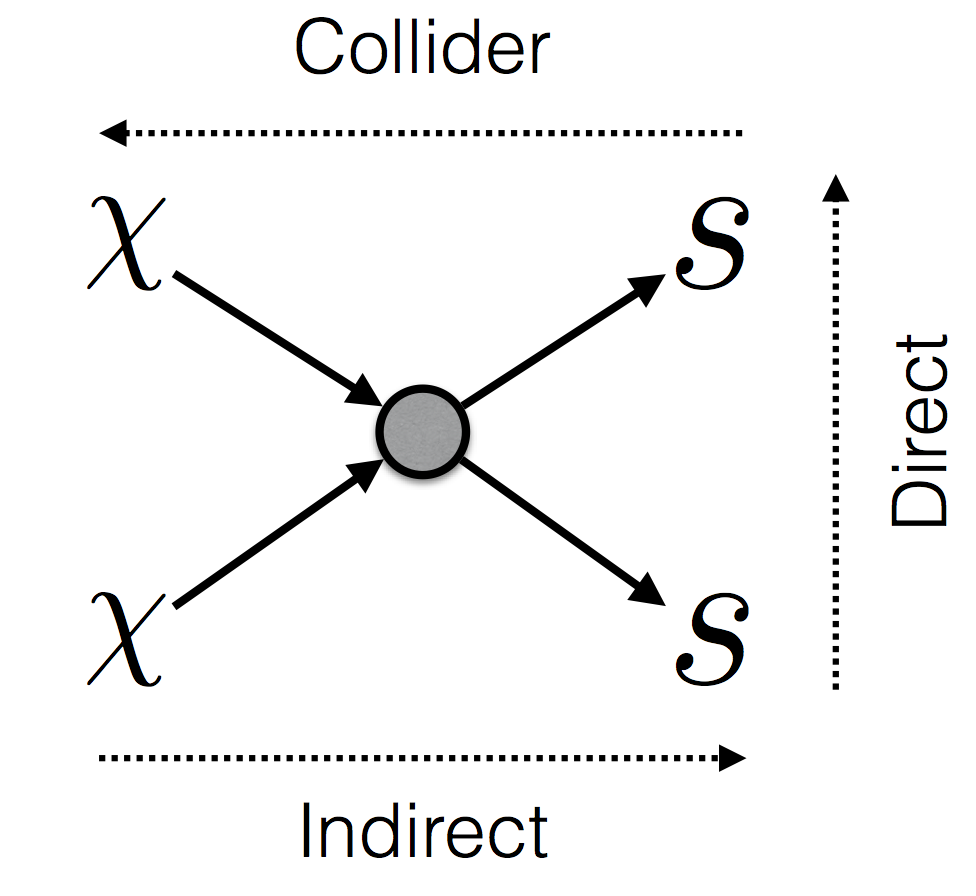
\includegraphics[width=0.45\textwidth]{images/3waystodetect/3waystodetect.pdf}
      \caption[Three Search Techniques]{
        The three general search techniques for dark matter.
        The $\chi$ is a dark matter particle, while $S$ is a standard model particle.
      }
      \label{fig:3_searches}
    \end{figure}
    
    In collider searches, $SS \rightarrow \chi\chi$, missing transverse energy is sought as dark matter particles are not expected to interact with the detector.
    For direct searches, $\chi S \rightarrow \chi S$, sensitive particle detectors are built deep underground.
    When a WIMP scatters off of a nucleus within the detector, the nuclear recoil can be observed, through signals such as crystal phonons, excitation and release of photons, or ionization.
    Being underground shields the detectors from cosmic rays, which create background collisions that can mimic WIMP signals.
    For example, in liquid xenon detectors, WIMP particle collisions in the liquid produce UV photons and electrons, which are used to infer the presence of the WIMPS~\cite{direct_lux,direct_xenon}.
    Another type are cryogenic, which use pucks of germanium and silicon to measure WIMP collisions.
    These collisions produce detectable ionization and phonon signals, which are used to classify the incident particle~\cite{direct_cdms}.
    A third example are scintillation detectors, which are built with crystals such as titanium-doped sodium iodine.
    When a WIMP collides with one of the nuclei within the crystal, that nucleus becomes excited, and then relaxes by releasing a photon~\cite{direct_dama}.
    However, to date no substantial dark matter signal has been detected with these methods~\cite{direct_dm_detection}.
    
    For indirect searches, $\chi\chi \rightarrow ss$, dark matter particles may annihilate or decay into standard model particles.
    Observatories then search for excesses of these particles, excesses that cannot be explained by currently understood astrophysics.
    This analysis searches for an excess of gamma rays, as the center of our galaxy is believed to host a dark matter halo.
    This spherical halo would allow for many $\chi\chi$ annihilations, producing gamma rays with
    
    $$\chi\bar{\chi} \rightarrow S\bar{S} \,,$$
    where $S\bar{S}$ can be any particle-antiparticle pair ($t\bar{t}$, $b\bar{b}$, $u\bar{u}$, $s\bar{s}$, \Pelectron{}\APelectron{}, \Pnue{}\APnue{}, \Pgg{}\Pgg{}, \Pg{}\Pg{}, \PHiggslight{}\PHiggslight{}, etc).
    The particle-antiparticle pairs then annihilate or decay into different spectra of photons ($\gamma$).
    These different annihilation channels can produce different spectra of gamma rays, which will also vary based on the WIMP mass and cross section chosen.
    This is described further in Section \ref{dm_spectral}.

\FloatBarrier

\section{Galactic Center}\label{sec:gc}
  
  The Galactic Center is a complex region of space, with many astrophysical sources of gamma rays.
  At its heart, kinematic observations of nearby stars have been used to infer the presence of a supermassive black hole, with a mass of \SI{4e6}{ M${{}_\odot}$ }\cite{sgra_massdist}.
  Around this black hole, gamma ray emission is observed~\cite{gc_pointsrc_hess,gc_pointsource_hess2,gc_veritas_pointsource,gc_magic_pointsource}, though the production mechanism is still debated.
  There are other gamma-ray sources as well, including dust along the galactic plane and supernova remnants.
  The TeV gamma-ray emission from a few of these sources is visible in Figure~\ref{fig:hess_plane}.
  
  \begin{figure}[!t]
    \centering
    %\includegraphics[width=0.98\textwidth]{images/hess_plane_survey/survey.pdf}
    %\caption[HESS GC Survey]{
    %  Significance map of the Galactic Center, from the HESS Galactic Plane Survey~\cite{hess_gc_plane}.
    %  \CaptionBlankLine
    %}
    \includegraphics[width=0.85\textwidth]{images/hess_galactic_plane_survey/survey.pdf}
    \caption[HESS GC Survey]{
      Flux map of the Galactic Center above \SI{1}{\TeV}, from the H.E.S.S. Galactic Plane Survey~\cite{hess_gc_plane2}.
      \CaptionBlankLine
    }
    \label{fig:hess_plane}
  \end{figure}
  
  \begin{figure}[!b]
    \centering
    \includegraphics[width=0.95\textwidth]{images/veritas_gc_ridge/ridge.pdf}
    \caption[VERITAS View of the Galactic Center Ridge]{
      Galactic Center Ridge, from Ref.~\cite{VeritasGCRidge2015}.
      \CaptionBlankLine
    }
    \label{fig:veritas_gc_ridge}
  \end{figure}

  The VERITAS significance sky map of this Galactic Center region is shown in Figure~\ref{fig:veritas_gc_ridge}.
  While a dark matter interpretation of this gamma-ray emission is intriguing~\cite{hessgcul}, there are several non-dark-matter models that might explain the observed features.
  %While a dark matter interpretation of this gamma-ray emission is intriguing~\cite{gc_pnt_is_dm1,gc_pnt_is_dm2}, there are several non-dark-matter models that might explain the observed features.
  One model that explains this TeV emission is that the supermassive black hole accelerates protons to PeV energies, which then collide with local atoms to produce \Ppizero{}s, which then decay into TeV gamma rays~\cite{gc_pevatron}.
  The second possibility suggests a nearby population of pulsars may be accelerating electrons, which then upscatter local photons to TeV energies~\cite{HooperTeVMSP}. %\cite{gc_pulsars,gc_pnt_is_not_dm2,gc_pnt_is_not_dm3}.
  The debate between these two models is currently ongoing~\cite{gc_pev_or_pwn}.
  Due to their limited angular resolution, the current generation of gamma-ray telescopes can only resolve the Galactic Center's gamma ray emission as a point source~\cite{VeritasGCRidge2015,gc_pointsrc_hess}.
  The Fermi telescope has observed a similar source of GeV gamma rays around the Galactic Center~\cite{gc_fermi_dm}, though neither the dark matter or pulsar explanations are completely conclusive~\cite{fermi_gc_pulsar_vs_dm,hoopergc}.
  
  In addition to this central source, there are also other sources of gamma rays in the vicinity.
  One of these sources is a disk of dust along the galactic plane, acting as an interaction medium for proton cosmic rays~\cite{diffusegamma1989}.
  These proton-proton collisions then produce neutral pions, which decay into gamma rays~\cite{gc_pevatron,Yoast_Hull_2014,hess_gc_diffuse}.
  High energy electrons scattering off of nuclei can also produce gamma rays via Bremsstrahlung.
  Gamma rays around the Galactic Center can also be produced by inverse Compton scattering.
  This occurs due to the upscattering of optical, infrared, and cosmic microwave background photons.
  These photons are upscattered by electrons accelerated in nearby sources such as pulsar wind nebulae.
  Supernova remnants can also produce gamma rays, as their expanding shells interact with ambient dust. 
  The extended emission from inverse Compton, pion decay, and supernovae processes are not modeled in this analysis.
  This is because the atmosphere's lack of uniformity overwhelms any diffuse emission in the residual sky maps\footnote{These residual maps are discussed in Section~\ref{subsec:likemax}.}.


\section{Indirect Dark Matter Search}
  For this analysis, it is necessary to understand how a terrestrial telescope can detect the presence of dark matter.
  Imaging atmospheric Cherenkov telescopes like H.E.S.S., MAGIC, and VERITAS can indirectly search for dark matter.
  These observatories attempt to detect gamma rays that are emitted when two dark matter particles annihilate.
  Because the rate of annihilation depends on the local dark matter density, the gamma-ray emission rate is affected by the radially-dependent structure of the dark matter halo.

  \subsection{Dark Matter and Gamma Rays}
    Primarily, indirect searches focus on annihilating WIMPs, as the predicted decaying WIMP produces a lower flux of standard model particles than annihilation.
    WIMPs may annihilate into any standard model particle-antiparticle pair, but most studies examine a WIMP annihilating into a quark-antiquark or gamma-ray photon pair~\cite{pdg2016}.
    These different annihilations produce different spectra of final gamma rays.
    The final spectrum of gamma rays used in this analysis is calculated in Section~\ref{dm_spectral}.
    After the gamma-ray spectrum is understood, the spatial distribution of the annihilations is also discussed in Section~\ref{dm_spatial}.
    The expected flux of gamma rays from a halo can then be calculated by combining these spatial and spectral models.
  
  \subsection{Spectrum of Gamma Rays from WIMP Annihilations}\label{dm_spectral}
    
    %   Fragmentation fractions of b quarks into weakly decaying 
    %   b-hadron species in Z->b\bar{b} decay, in p\bar{p} collisions at sqrt(s)=1.96 TeV
    %   http://pdg.lbl.gov/2018/reviews/rpp2018-rev-b-meson-prod-decay.pdf
    %   pg4: Table 85.1
    %   b Hadron  | Fraction at Z [%] | Fraction at p\bar{p}
    %   B+,B^0    |       41.2 ± 0.8  |  34.0 ± 2.1 
    %   B_s       |        8.8 ± 1.3  |  10.1 ± 1.5
    %   b baryons |        8.9 ± 1.2  |  21.8 ± 4.7
    
    % B^+ (ub_) Decay Modes http://pdg.lbl.gov/2018/listings/rpp2018-list-B-plus-minus.pdf
    %   -> \bar{D}^0 X : 79   ± 4
    %   -> D^- X       :  9.9 ± 1.2
    %   -> D^0 X       :  8.6 ± 0.7
    % B^- (u_b) Decay Modes (charge conjugates of B^+)
    %   -> D^0 X       : 79   ± 4
    %   -> D^+ X       :  9.9 ± 1.2
    %   -> \bar{D}^0 X :  8.6 ± 0.7
    % B^0 (d_b) Decay Modes http://pdg.lbl.gov/2018/listings/rpp2018-list-B-zero.pdf
    %   -> K^± anything : 78   ± 8
    %   -> \bar{D}^0 X  : 47.4 ± 2.8
    %   -> D^- X        : 36.9 ± 3.3
    %   -> D^0 X        :  8.1 ± 1.5
    
    % D^+ (cd_) Decay Modes http://pdg.lbl.gov/2018/tables/rpp2018-tab-mesons-charm.pdf
    %   -> \bar{K}^0 anything + K^0 anything : 61    ± 5
    %   -> K^- anything                      : 25.7  ± 1.4
    %   -> \mu^+ anything                    : 17.6  ± 3.2
    %   -> e^+ semileptonic                  : 16.07 ± 0.30
    %   -> \bar{K}^0 \mu^+ \nu_{\mu}         :  8.74 ± 0.19
    %   -> \bar{K}^0 e^+ \nu_e               :  8.73 ± 0.10
    % D^- (c_d) Decay Modes (charge conjuages of D^+)
    %   -> \bar{K}^0 anything + K^0 anything : 61    ± 5
    %   -> K^+ anything                      : 25.7  ± 1.4
    %   -> \mu^- anything                    : 17.6  ± 3.2
    %   -> e^- semileptonic                  : 16.07 ± 0.30
    %   -> \bar{K}^0 \mu^- \bar{\nu}_{\mu}   :  8.74 ± 0.19
    %   -> \bar{K}^0 e^-   \bar{\nu}_e       :  8.73 ± 0.10
    % D^0 (cu_) http://pdg.lbl.gov/2018/tables/rpp2018-tab-mesons-charm.pdf
    %   -> \bar{K}^0 anything + K^0 anything : 47   ± 4
    %   -> K^- anything                      : 45.7 ± 2.8
    %   -> K^- \pi^+ \pi^0                   : 14.2 ± 0.5
    %   -> K^- \pi^+ \pi^+ \pi^-             : 8.11 ± 0.15
    
    % K^+ (s_u) Decay Modes http://pdg.lbl.gov/2018/tables/rpp2018-tab-mesons-strange.pdf
    %   -> \mu^+ \nu_{\mu}       : 63.56 ± 0.11
    %   -> \pi^+ \pi^0           : 20.67 ± 0.08
    % K^- (su_) Decay Modes (charge conjugate of K^+)
    %   -> \mu^- \bar{\nu}_{\mu} : 63.56 ± 0.11
    %   -> \pi^- \pi^0           : 20.67 ± 0.08
    % K^0 (s_d) Decay Modes (http://pdg.lbl.gov/2018/listings/rpp2018-list-K-zero.pdf
    %   -> 
    % K^0_S Decay Modes 
    %   -> \pi^0 \pi^0 : 30.69 ± 0.05
    %   -> \pi^+ \pi^- : 69.20 ± 0.05 
    % K^0_L Decay modes
    %   -> \pi^± e^∓ \nu_e       : 40.55 ± 0.11
    %   -> \pi^± \mu^∓ \nu_{\mu} : 27.04 ± 0.07
    %   -> \pi^0 \pi^0 \pi^0     : 19.52 ± 0.12
    %   -> \pi^+ \pi^- \pi^0     : 12.54 ± 0.05
    
    % \pi^0 Decay Modes http://pdg.lbl.gov/2018/listings/rpp2018-list-pi-zero.pdf
    %   -> \gamma \gamma  : 98.823 ± 0.034
    
    % b->B mesons
    
    In order to calculate the gamma-ray brightness of the dark matter halo, the produced gamma-ray energy spectrum from WIMP annihilations must be known.
    Different annihilation channels can produce different spectra.
    For instance, the $\chi\chi \rightarrow \gamma\gamma$ channel will produce a spectrum with a single spike at the WIMP's mass, while the $\chi\chi \rightarrow \bbbar{}$ channel will produce a curved power law spectrum of photons, shown in Figure~\ref{fig:chichi_spectrum}.
    WIMP annihilations are expected to have multiple channels, where a population of WIMPs will annihilate into different channels with different probabilities.
    However, only the $\chi\chi \rightarrow \bbbar$ channel is considered for this analysis.
    
    Three example Feynman diagrams of WIMP annihilations that produce a \bbbar pair are shown in Figure~\ref{fig:neutralino_feynman}, adapted from Ref.~\cite{Jungman:1995df}.
    The particle $\tilde{f}$ is a supersymmetric fermion, the $Z$ is the Z boson, and $H$ is Higgs boson.
    The analysis in this thesis searches for a general \bbbar signal, rather than the specific signal from one of these Feynman diagrams.
    
    \begin{figure}[h]
      \centering
      \hfill
      \begin{minipage}{0.17\textwidth}\includegraphics[width=\linewidth]{images/feynman_neutralino/neutralino_superf.pdf}\end{minipage}\hfill
      \begin{minipage}{0.25\textwidth}\includegraphics[width=\linewidth]{images/feynman_neutralino/neutralino_zboson.pdf}\end{minipage}\hfill
      \begin{minipage}{0.25\textwidth}\includegraphics[width=\linewidth]{images/feynman_neutralino/neutralino_aghost.pdf}\end{minipage}\hfill
      \hfill
      \caption[WIMP Annihilation Feynman Diagrams]{
        Three example Feynman diagrams of neutralino annihilations that produce a \bbbar pair.
      }
      \label{fig:neutralino_feynman}
    \end{figure}

    After the desired channel is selected, the spectrum of photons produced by that channel is calculated.
    This is done by repeatedly simulating all the photons produced when the \bbbar quarks hadronize and decay into other particles.
    Several of these decay processes are shown in Table~\ref{tab:bpaths2}.
    In the table, the $\bar{b}$ hadronizes into \PBplus or \PBzero, which then decay into \PK and \PD mesons (plus some other particles $X$), and the \PD mesons also decay into \PK mesons.
    The \PK mesons can then decay into \Ppipm and \Ppizero mesons, and finally the \Ppizero{}'s decay into two photons.
    % for pion decays, see section 3.3 in arxiv:1508.05190 (and references therein)
    Though these pion decays are the dominant source of photons, these listed particles (as well as other unlisted ones) may produce additional photons through bremsstrahlung or annihilation mechanisms.
    All of the photons produced from pion decays, bremsstrahlung, and annihilations then make up a gamma-ray spectrum that is used in this analysis.
    
    \begin{table}
      \centering
      \begin{tabular}{ccll}
        Source                       & Branching                       & Products       & PDG \\
        (Quarks)                     & Ratio (\%)                      &                & Chapter \\ \hline
        $\bar{b}$                    & $\xrightarrow{ \mathrm{Hadronization} }$   & \PBp, \PBz     & \href{http://pdg.lbl.gov/2018/reviews/rpp2018-rev-b-meson-prod-decay.pdf}{$b$-Hadron Production}              \\ \hline
        \PBp     $(u\bar{b})$   & $\xrightarrow{ 79   \pm4   }$   & $\APDzero + X$ & \href{http://pdg.lbl.gov/2018/listings/rpp2018-list-B-plus-minus.pdf}{Charged B Mesons}          \\
        \PBz     $(d\bar{b})$ & $\xrightarrow{ 78   \pm8   }$   & $\PKpm + X$    & \href{http://pdg.lbl.gov/2018/listings/rpp2018-list-B-zero.pdf}{Neutral B Mesons}          \\
        \PBz     $(d\bar{b})$ & $\xrightarrow{ 47.4 \pm2.8 }$   & $\APDzero + X$ & \href{http://pdg.lbl.gov/2018/listings/rpp2018-list-B-zero.pdf}{Neutral B Mesons}          \\
        \PBz     $(d\bar{b})$ & $\xrightarrow{ 36.4 \pm3.3 }$   & $\PDminus + X$ & \href{http://pdg.lbl.gov/2018/listings/rpp2018-list-B-zero.pdf}{Neutral B Mesons}          \\ \hline
        \APDzero $(u\bar{c})$    & $\xrightarrow{ 45.7 \pm2.8 }$   & $\PKplus + X$  & \href{http://pdg.lbl.gov/2018/tables/rpp2018-tab-mesons-charm.pdf}{Charm Mesons}          \\
        \PDminus $(d\bar{c})$  & $\xrightarrow{ 25.7 \pm1.4 }$   & $\PKplus + X$  & \href{http://pdg.lbl.gov/2018/tables/rpp2018-tab-mesons-charm.pdf}{Charm Mesons}          \\ \hline
        \PKplus  $(u\bar{s})$  & $\xrightarrow{ 20.67\pm0.08}$   & $\Ppizero + \Ppiplus$  & \href{http://pdg.lbl.gov/2018/tables/rpp2018-tab-mesons-strange.pdf}{Strange Mesons} \\
        \PKminus $(\bar{u}s)$  & $\xrightarrow{ 20.67 \pm0.08 }$ & $\Ppizero + \Ppiminus$  & \href{http://pdg.lbl.gov/2018/tables/rpp2018-tab-mesons-strange.pdf}{Strange Mesons} \\ \hline
        \Ppizero $\left ( \frac{u\bar{u} - d\bar{d} }{\sqrt{2}} \right )$   & $\xrightarrow{ 98.823\pm0.034}$ & $\gamma + \gamma$ & \href{http://pdg.lbl.gov/2018/listings/rpp2018-list-pi-zero.pdf}{Neutral Pion} \\
        %$$ & $\xrightarrow{ \pm }$ & $$ \\
        %\APDzero    & $\xrightarrow{ 47  \pm4   }$ & $K^0 + \bar{K}^0 + anything $ \\
        %\PDminus    & $\xrightarrow{ 61  \pm5   }$ & $K^0 + \bar{K}^0 + anything$ \\
        % Numbers are from  the beginning of this subsection
      \end{tabular}
      \caption[$b$ Quark Production of Gamma Rays]{
        Table of decay modes and products, indicating several ways photons are produced from $\bar{b}$ quarks.
        The $X$ indicates other particles.
        Branching ratios and Particle Data Group (PDG) chapters are from Ref.~\cite{tanabashi2018review}.
      }
      \label{tab:bpaths2}
    \end{table}
    
    %\begin{table}
    %\centering
    %\begin{tabular}{lcll}
      %Source      & Branch Fraction                         & Products                  & Ref.     \\
      %\hline
      %$\bar{b}$   & $\xrightarrow{59.8   \% \pm 2.9    \%}$ & $\bar{D}^{0} + \textrm{other}$ &  \cite{pdg_2012} \\
      %$\bar{D}^0$ & $\xrightarrow{54.7   \% \pm 2.8    \%}$ & $K^+         + \textrm{other}$ &  \cite{pdg_2008} \\
      %$K^+$       & $\xrightarrow{63.56  \% \pm 0.11   \%}$ & $\mu^+ + \nu_{\mu}$            &  \cite{pdg_2014} \\
      %\hline
      %$\bar{b}$   & $\xrightarrow{23.3   \% \pm 1.7    \%}$ & $D^-   + \textrm{other}$       &  \cite{pdg_2012} \\
      %$D^-$       & $\xrightarrow{25.7   \% \pm 1.4    \%}$ & $K^+   + \textrm{other}$       &  \cite{pdg_2008} \\
      %$K^+$       & $\xrightarrow{63.56  \% \pm 0.11   \%}$ & $\mu^+ + \nu_{\mu}$            &  \cite{pdg_2014} \\

      %$K^+$     & $\xrightarrow{20.67  \% \pm 0.08   \%}$ & $\pi^0 + \pi^+$                &  \\
      %$\pi^0$   & $\xrightarrow{98.798 \% \pm 0.032  \%}$ & $\gamma + \gamma$              &  \\
      %$\pi^+$   & $\xrightarrow{99.9877\% \pm 0.00004\%}$ & $\mu^+ + \nu_{\mu}$            &  \\
      %Hadronization & $\bar{b}$ & $\xrightarrow{40.1   \% \pm 0.8    \%}$ & $B^+$                     &  \cite{pdg_2012} \\
      %Decay         & $B^+$     & $\xrightarrow{10.99  \% \pm 0.28   \%}$ & $l^+ + \nu_l + \other$    &  \cite{pdg_2014} \\
      %\hline
      %Hadronization & $\bar{b}$ & $\xrightarrow{40.1   \% \pm 0.8    \%}$ & $B^0$                     &  \cite{pdg_2012} \\
      %Decay         & $B^0$     & $\xrightarrow{10.33  \% \pm 0.28   \%}$ & $l^+ + \nu_l$             &  \cite{pdg_2014} \\
      %\hline
      %Hadronization & $\bar{b}$ & $\xrightarrow{ 9.3 \% \pm 1.6 \%}$ & $\bar{b}\bar{q}\bar{q}$   \\
      %Hadronization & $\bar{b}$ & $\xrightarrow{10.5 \% \pm 0.6 \%}$ & $B^0_S$                \\
      %$\bar{b}$ & $\xrightarrow{17.3 \% \pm 2.0 \%}$ & $D^{*}(2010)^{+} + \any$ & \\
      %$D^0$     & $\xrightarrow{6.53 \% \pm 0.17\%}$ & $e^{+}           + \any$ & \\
      %$D^0$     & $\xrightarrow{6.7  \% \pm 0.6 \%}$ & $\mu^{+}         + \any$ & 
      %Decay & $D^0$     & $\xrightarrow{47   \% \pm 4   \%}$ & $\bar{K}^0 + K^0 + \any$     & inclusive \\
      %Decay & $D^-$     & $\xrightarrow{61   \% \pm 5   \%}$ & $\bar{K}^0 + K^0 + \any$     & inclusive \\
    %\end{tabular}
    %\caption[$b$ Quark Production of Photons]{
      %Table of decay modes and products, indicating two ways ways a lone $b$ quark can indirectly produce photons.
      %The $\mu^+$ is then able to produce bremsstrahlung photons.
      %The charge conjugate of the source is assumed to charge conjugate the products.
      %Constituent quarks for particles are $\bar{D}^0=\bar{c}u$, $K^+=u\bar{s}$, and $D^-=\bar{c}s$.
      %$B^+=u\bar{b}$, $B^0=d\bar{b}$, $B^0_S=s\bar{b}$, $D^0=c\bar{u}$, $K^-=\bar{u}s$, $\pi^0=\frac{u\bar{u}-d\bar{d}}{\sqrt{2}}$, and $\pi^+=u\bar{d}$.
      %}
    %\label{tab:bpaths}
    %\end{table}
    
    The software package CLUMPY~\cite{CLUMPYcode} is used in this thesis to calculate the gamma-ray spectra for each annihilation channel.
    The spectral models that CLUMPY uses are based on the annihilation spectra in the PPPC 4 DM ID~\cite{pppc4_dm_spectra,pppc4_ewcorrections}.
    These spectra are calculated using Monte Carlo simulations performed with PYTHIA~\cite{pythia} and HERWIG~\cite{herwig}.
    Figure~\ref{fig:chichi_spectrum} shows the resultant spectra from the annihilation of two WIMPs.
    Each line shows the spectrum from a different initial WIMP mass.

    \begin{figure}[bt]
      \centering
      \includegraphics[width=0.95\textwidth]{images/spectra/chichi_spectrum.pdf}
      \caption[Single Annihilation Spectra]{
        Resultant photon spectra from the annihilation of two WIMP particles solely into the \bbbar channel.
        Each colored line represents a different WIMP mass.
      }
      \label{fig:chichi_spectrum}
    \end{figure}

    These spectra can be combined with the J-factor (Equation~\ref{eqn:jfactor}) to calculate the gamma-ray flux produced by the halo (Equation~\ref{eqn:dmflux}).
    It is important to note that mass-to-light ratios, and their derived J-factors are usually inferred from measuring star spectra.
    These measured J-factors can therefore suffer from large errors, as it can be difficult to determine which stars are within a target gravitational well, and which ones are foreground or background stars~\cite{segue_jfactor_errors}.
    
    By using estimated parameters with Equation~\ref{eqn:dmflux}, the flux of gamma rays from a dark matter halo can be estimated in order to understand how few events a dark matter halo produces.
    The flux of gamma rays from a dark matter halo can be estimated with Equation~\ref{eqn:dmflux} to understand how just how few gamma rays can be observed from a dark matter halo.
    For this estimate, the dark matter mass is chosen to be \SI{10}{\TeV{}}, and the velocity-averaged cross section $\left < \sigma v \right >$ is set at the relic cross section.
    Other chosen parameters are specified in Table~\ref{tab:halo_nphotons}, to align with the VERITAS telescope performance, or the parameters of the dark matter analysis performed in later chapters.
    For the table parameters, the dark matter halo would only produce a VERITAS-observable gamma ray between \SIrange{4}{10}{\TeV{}} every 39 hours.
    This flux $\Phi$ is proportional to the $\sv$, so a factor of $n$ larger particle cross section would produce a factor of $n$ larger photon flux.
    Another way to increase the observed photon flux is by expanding the observable gamma-ray energy range.
    If the entire VERITAS energy range of \SIrange{1.5}{70}{\TeV{}} is used, the observable halo photon energy range expands to \SIrange{1.5}{10}{\TeV{}}, so the integrated photon spectrum increases, and the observed halo photon flux increases by a factor of 26.
    
    \begin{table}[]
      \centering
      \begin{tabular}{r|l}
        \hline
        \textbf{Estimated Parameters}            & \\
        $m_{\chi}$                               & \SI{10}{\TeV{}}           \\
        Relic velocity-averaged cross section $\vacs$ & \SI{3e-26}{cm^3/s}   \\
        Field of view                            & \ang{3}                   \\
        %VERITAS detectable photon energy range   & \SIrange{1.5}{70}{\TeV{}} \\
        %Analysis photon energy range             & \SIrange{4}{70}{\TeV{}}   \\
        %Maximum dark matter halo photon energy   & \SI{10}{\TeV{}}           \\
        Observable halo photon energy range      & \SIrange{4}{10}{\TeV{}}\tablefootnote{
          At \ang{30} elevation, the VERITAS detectable photon energy range is \SIrange{1.5}{70}{\TeV{}}.
          However, the analysis is limited to \SIrange{4}{70}{\TeV{}}, and through conservation of energy, dark matter annihilations can't produce photons higher than the mass of the dark matter particle, \SI{10}{\TeV{}} in this example.
          Thus, the final observable energy range is \SIrange{4}{10}{\TeV{}}.
          }   \\
        Observatory effective area               & \SI{287000}{m^2}          \\
        Annihilation channel                     & $\chi\chi \rightarrow \bbbar $ \\
        Dark matter halo shape                   & Einasto              \\
        \hline
        \textbf{Derived Values}                  & \\
        Integrated photon spectrum : $\int \frac{dN_{\gamma}}{dE} dE$        & 0.00536 photons per $\chi\chi$ annihilation \\
        J-factor :$\int \int \rho^2 dl\,d\Omega$ & \SI{3.88e22}{\GeV{}^2/cm^5}      \\
        Halo flux $\Phi$                         & \SI{2.5e-11}{photons/(s*m^2)} \\
        One halo photon detected every           & \SI{39}{hours} \\
        \hline
      \end{tabular}
      \caption[Halo Model Parameters]{
        Number of gamma rays from a dark matter halo.
        Field of view is the radial field of view of VERITAS.
        Observatory effective area is the VERITAS effective area at \ang{29} telescope elevation (the average elevation of Galactic Center at VERITAS's latitude), \ang{0.5} offset from GC, at the $\log_{10}$ mean energy (\SI{16.7}{\TeV{}}) in the selected energy range.
        The Einasto halo shape parameters are chosen to be the same as in Section~\ref{dm_spatial}.
      }
      \label{tab:halo_nphotons}
      % values derived with $VERIPY/thesis/analysis/example_dm_halo_photons/example.py
    
    \end{table}

    \FloatBarrier

  \subsection{Dark Matter Halo Structure}\label{dm_spatial}
    
    Observations allow most galactic dark matter halos to be modeled using a class of similar density profiles.
    A currently favored profile is the Einasto profile~\cite{einastoprofile1,einastoprofile2}.
    This profile describes the mass-density of dark matter at a distance $r$ from the halo center, $\rho(r)$.
    The Einasto profile is described by

    \begin{equation} \label{eqn:einasto}
      \rho_{\textrm{DM}} \left( r \right) = \rho_{s} Exp \left( - \frac{2}{\alpha} \left( {\left( \frac{r}{r_s} \right)}^{\alpha} - 1 \right) \right) \,,
    \end{equation}
    where $r_s$ is the scale radius of the halo, which specifies how wide the dark matter halo is.
    The parameter $\rho_s$ is the scale density, which is the dark matter density at the scale radius.
    The parameter $\alpha$ is the power of the density profile's slope.
    
    A larger $\alpha$ reduces the dark matter densities above and below the scale radius $r_s$.
    Both $\alpha$ and $r_s$ are from the best fit values of the Aq-A-1 simulation in Table 2 of Ref.~\cite{mw_halo_params}.
    The $r_s$ parameter is calculated via $r_s=r_{-2}=15.14\:\textrm{kpc}$, where $r_{-2}=\frac{11.05}{h_{73}}\:\textrm{kpc}$ (in Ref.~\cite{mw_halo_params}, Table 2) and $h_{73}=0.73$ from Section 2.1 in Ref.~\cite{mw_halo_params}.
    In the model, the parameter $\alpha$ is fixed to 0.17, and $r_s$ is fixed to \SI{15.14}{kpc}.
    The distance to the Galactic Center is known to be $r_\odot=8\:\textrm{kpc}$~\cite{gc_distance_1,gc_distance_2,gc_distance_3}.
    The assumed Milky Way mass profile has a mass density of $\rho_\odot = 0.4\:\frac{\textrm{GeV}}{\textrm{cm}^3}$~\cite{local_dm_density,direct_dm_astrophysical_uncertainties}.
    Since $r_\odot$ and $\rho_\odot$ are known, then in Equation~\ref{eqn:einasto} the dark matter density at the scale radius $\rho_s$ is derived to be \SI{0.12}{\GeV{}\per\cm^3}.
    With these values, the Einasto profile in Equation~\ref{eqn:einasto} is shown in Figure~\ref{fig:gchalo_density}.
    The distribution of dark matter follows an Einasto profile.
  
    \begin{figure}[!t]
      \centering
      %\includegraphics[width=0.85\textwidth]{images/halo/gc_einasto_profile.pdf}
      \includegraphics[width=0.85\textwidth]{images/halo_corrected/mass_density/gc_einasto_profile.pdf}
      \caption[Galactic Center Einasto Halo Density]{
        Mass density of the Einasto dark matter halo (Equation~\ref{eqn:einasto}) used in this analysis.
        The bottom x axis shows the angle (as viewed from Earth) from the Galactic Center, while the top x axis shows the distance from the Galactic Center in kiloparsecs.
        \CaptionBlankLine
        }
      \label{fig:gchalo_density}
    \end{figure}

    
    Most n-body simulations predict that density profiles steeply rise as $r \rightarrow 0$, forming a peak or \textit{cusp} at their center.
    However, observations of dwarf galaxies usually show a flat density core within a given radius~\cite{flores1994observational,CoreVsCusp}.
    This may be due to the presence of baryons in this core region, which can diffuse the central cusp of WIMPs into a core-like shape~\cite{corecusp_baryondiffuse1,corecusp_baryondiffuse2}.
    As this flat core occurs in the innermost region covered by the gamma-ray observations in this analysis, the choice of a cusped or cored dark matter halo can have a significant impact.
    Specifically, if the true dark matter halo has a cored profile, but is modeled using a cusped one, then any derived upper limits on the dark matter cross section would be different.
    As a basic first step, only a cusped halo is used in this thesis.
    
    When choosing which dark matter target to observe with a gamma-ray observatory, knowing the gamma-ray brightness of different sources can be useful.
    This Einasto density profile can be integrated to calculate the gamma-ray brightness, independent of the WIMP model being searched for.
    For annihilating dark matter, $\rho_{\textrm{DM}}\left(r\right)^2$ must be integrated along the line of sight.
    
    The flux of gamma rays produced by these annihilations is given by
    
    \begin{equation}\label{eqn:dmflux}
      \frac{ d\Phi }{ dE d \Omega } = \frac{ \left \langle \sigma v \right \rangle }{8 \pi m_\chi^2} \frac{dN_{\gamma}}{dE} \int \rho^2 dl \, ,
    \end{equation}
    where the photon flux $\Phi$ is the number of gamma rays detected per $\textrm{area}\times\textrm{time}$.
    The velocity-averaged cross section of the dark matter candidate is $\left \langle \sigma v \right \rangle$.
    Velocity-averaging is used because the cross section is velocity dependent, and the WIMPs that pass through a volume of space will have a distribution of velocities~\cite{wimp_veldist}.
    The average spectrum of photons produced by a single $\chi\chi$ annihilation is $\frac{dN_{\gamma}}{dE}$.
    The density integral in Equation~\ref{eqn:dmflux} with the solid angle $d\Omega$ differential is often calculated separately, and is referred to as the J-factor,

    \begin{equation}\label{eqn:jfactor}
      J = \int \rho^2 dl\,d\Omega \;\; .
    \end{equation}

    The J-factor is used to compare the relative gamma-ray brightness of different dark matter halos, which is a function of both dark matter density and observing distance.
    The Einasto density in Equation~\ref{eqn:einasto} can be integrated to calculate the J-factor at various radii, which is shown in Figure~\ref{fig:gchalo_jfactor}.
    In Figure~\ref{fig:gchalo_jfactor}, the profile shown is calculated with Equation~\ref{eqn:jfactor}, where the $d\Omega$ integration limits span an angle of \ang{0.06}.
    % integration angle of 0.06 deg
    % low-res halo template used NSIDE=1024, 
    % and ALPHA_INT (angle of integration) was calculated from NSIDE, via
    % healpy.max_pixrad(1024) = 0.00104 radians = 0.0598 deg ~= 0.06 deg
    This J-factor profile then forms the spatial component of the dark matter halo, $M_{s,\textrm{halo}}$, used in Chapter~\ref{chapter:analysis}.
    This profile is shown in a two-dimensional plot in Figure~\ref{fig:halojfactor}.
    
    \begin{figure}[!t]
    \centering
      %\includegraphics[width=0.85\textwidth]{images/halo/gc_einasto_jfactor.pdf}
      \includegraphics[width=0.85\textwidth]{comments/jfactor_plots/alternate_scaled_plot/output/calc_Jfactor_per_deg2.pdf}
      \caption[Galactic Center Einasto Halo J-Factor]{
        J-factor profile as a function of angle from the Galactic Center, calculated via Equation~\ref{eqn:jfactor} with the Einasto density profile in Equation~\ref{eqn:einasto}.
        The J-factor values are calculated by integrating \ang{0.06} around each angle from the Galactic Center.
      }
      \label{fig:gchalo_jfactor}
    \end{figure}
  
  \begin{figure}[!t]
    \centering
    %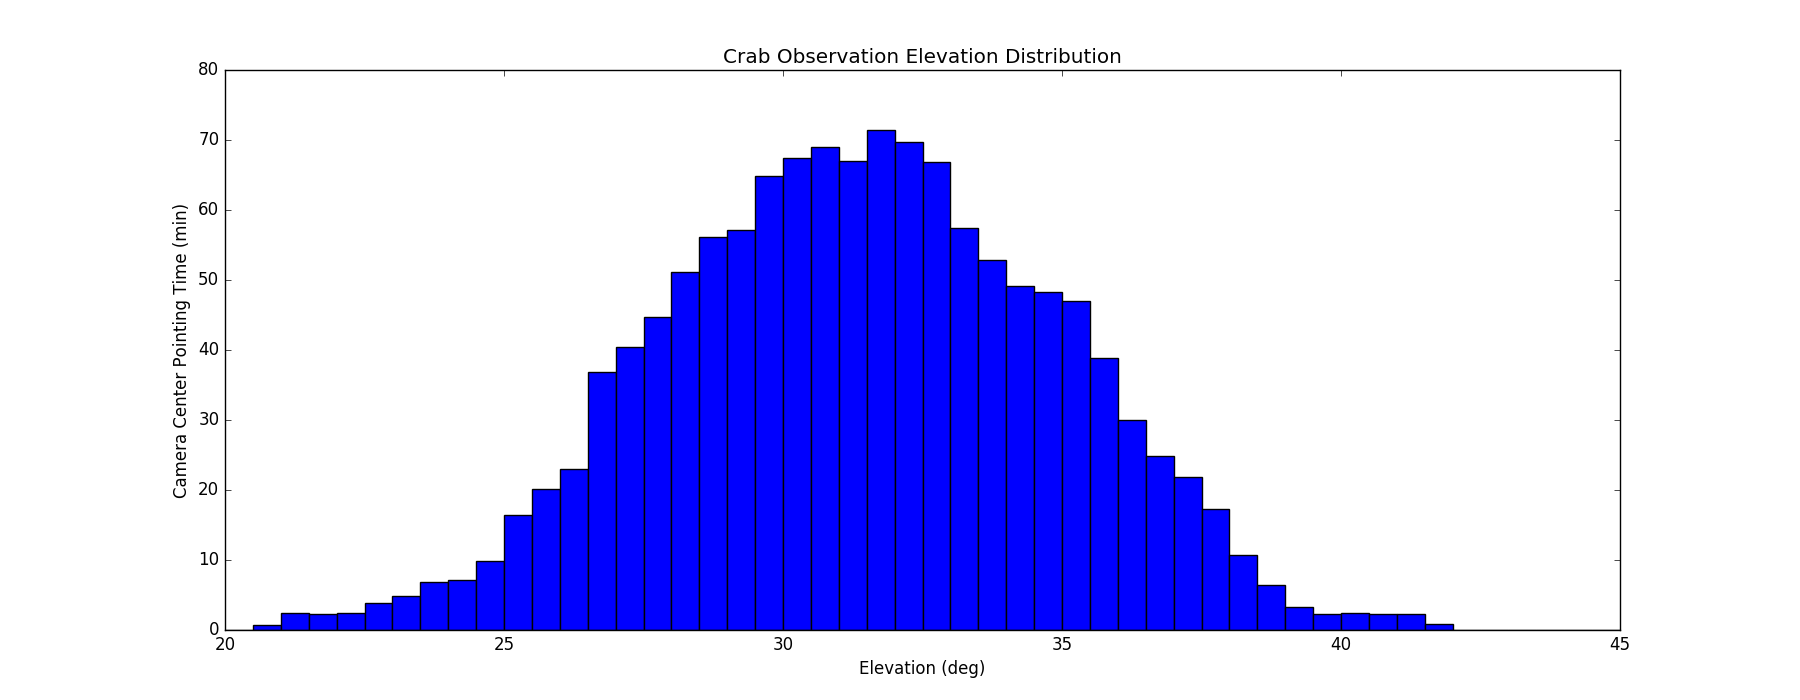
\includegraphics[width=0.85\textwidth]{images/halo_flux/plot.pdf}
    \includegraphics[width=0.85\textwidth]{comments/jfactor_plots/alternate_scaled_plot/output/calc_skymap.pdf}
    \caption[Galactic Center Halo J-Factor Sky Map]{
      J-factor of the dark matter halo model used in this analysis.
      The green circles indicate the different observation regions.
      Note this is showing the same model as Figure~\ref{fig:gchalo_jfactor}, except here the J-factor axis is linear instead of logarithmic.
      The black corners result from the halo model only being calculated out to a radius of \ang{3}, since there are no observations that extend past that.
      The halo center is positioned at Sgr A*, which is at $$(l,b)_{\textrm{J2000}} = (\ang{359.944212}, \ang{-0.046013}) \,.$$
      It is not positioned at the origin $(0,0)$ because the $(l,b)$ coordinate system does not perfectly align with the Milky Way galaxy~\cite{galacticlb}.
      %It is not centered at $(l,b)=(0,0)$ because the $(l,b)$ coordinate system origin is not centered directly at Sgr A*.
      %The coordinate system is instead derived from a series of J2000 right ascension and declination reference points, which result in the origin only being accurate to $\pm$\ang{0.1}\cite{galacticlb}.
      % discussed further: https://en.wikipedia.org/wiki/Galactic_coordinate_system
    }
    \label{fig:halojfactor}
  \end{figure}

  The halo structure in Figure~\ref{fig:halojfactor} is a simple first step halo, one that does not account for more complex dark matter models.
  For example, a search for decaying dark matter would instead change the J-factor calculation to $\int \rho \, dl \, d\Omega \,$, spreading out the gamma-ray emission.
  More exotic WIMP models may slightly alter the gamma-ray brightness of the dark matter halo, compared to the previously mentioned WIMP model.
  For example, if dark matter WIMPs have an attractive force between them, their effective annihilation cross section is enhanced, increasing the gamma-ray emission from the halo.
  This effect is called Sommerfeld enhancement~\cite{sommerfeld}.
  % originally from http://inspirehep.net/record/1286230/files/Thesis-2009-Nierop.pdf
  % from http://www.pnas.org/content/112/40/12264.full.pdf
    
  
  \FloatBarrier
    
\section{Cherenkov Photons}\label{sec:cherenkov}

  Cherenkov light and its production is discussed in this section, because the detection of gamma rays in Section~\ref{sec:atmoshowers} relies heavily on knowledge of Cherenkov light.
  Within the Earth's atmosphere (or any dielectric medium), the phase velocity of light $c_{atmosphere}$ is slightly slower than in a vacuum.
  Any charged particles travelling at velocity $v > c_{atmosphere}$ will induce the atmosphere to produce Cherenkov photons~\cite{cherenkov}.
  From a single charged particle of constant velocity, Cherenkov photons form a conical wavefront shown in Figure~\ref{fig:cherenkovangle}.
  This wavefront is similar to a sonic boom shockwave, or the wake produced when a boat travels faster than the speed of the waves.

  \begin{figure}[!t]
    \centering
    \includegraphics[width=0.27\textwidth]{images/cherenkov_angle/cherenkovangle.pdf}
    \caption[Cherenkov Emission Angle]{
      Cherenkov light (blue arrows) is emitted at angle $\theta$, relative to the charged particle z's path.
    }
    \label{fig:cherenkovangle}
  \end{figure}

  Cherenkov photons are emitted at an angle $\theta$ relative to the charged particle's path, determined by the index of refraction of the medium $n$, the speed of the charged particle $v$, and the speed of light in the medium $c$:
  % showers are 10km up, light pool on ground is 130m diameter, \theta = ArcSin(130/10000) * 180 / pi = 0.73deg ~ 1deg

  \begin{equation}\label{eqn:cherenkovangle}
    \theta = ArcCos \left ( \frac{c}{n \; v} \right ) \,.
  \end{equation}
  
  For the air showers used in this analysis, the Cherenkov angle $\theta$ is \nicetilde\ang{1}.
  In practice, air showers are more complex due to the number and distribution of charged particles and their velocities, energy losses, and Cherenkov photons repeatedly scattering off of the atmosphere.
  These effects tend to smear the theoretically-clean Cherenkov cones into a diffuse pool of light on the ground, shown in Figure~\ref{fig:lightpool}.

  \begin{figure}[!t]
    \centering
    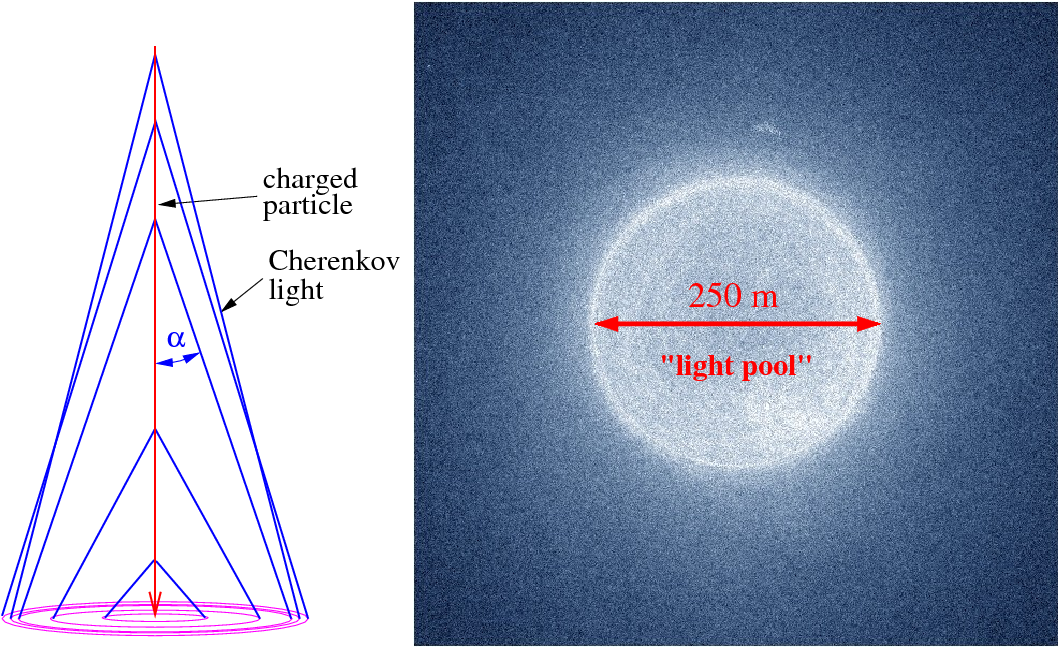
\includegraphics[width=0.85\textwidth]{images/lightpool/lightpool.pdf}
    \caption[Cherenkov Light Pool]{
      Cherenkov light from a gamma ray shower illuminating the ground.
      Due to the changing atmospheric density, the Cherenkov angle changes as the electromagnetic shower descends (left), concentrating the emitted light into a ring-like pool (right).
      The initial gamma ray in this simulated example had an energy of \SI{1}{\TeV{}}.
      Figure is from Ref.~\cite{Voelk}.
    }
    \label{fig:lightpool}
  \end{figure}
  
  The spectrum of photons produced by the Cherenkov effect can be calculated with the Frank-Tamm formula~\cite{franktamm1,franktamm2},
  
  \begin{equation}\label{eqn:franktamm}
    \frac{dE}{dx\,d\omega}=\frac{(ze)^2 \, \omega}{c^2} \left ( 1 - \frac{c^2}{v^2 \;\epsilon(\omega)} \right ) \,,
  \end{equation}
  where $E$ is the energy emitted as Cherenkov radiation, $x$ is the length of the charged particle path, $ze$ is the charge of the particle, $\omega$ is the emitted Cherenkov photon frequency, $c$ is the speed of light (phase velocity) in the medium, $v$ is the speed of the particle, and $\epsilon(\omega)$ is the frequency-dependent permittivity.
  
  \begin{figure}[!t]
    \centering
    \includegraphics[width=0.65\textwidth]{images/CherenkovReactor/cherenkovreactor.eps}
    \caption[Cherenkov Light from a Reactor]{
      Blue Cherenkov light in the Advanced Test Reactor core, at the Idaho National Laboratory~\cite{cherenkovreactor,atrlab}.
    }
    \label{fig:cherenkovreactor}
  \end{figure}
  
  In Figure~\ref{fig:cherenkovreactor}, a visible example of Cherenkov photons is shown, produced in the Advanced Test Reactor at the Idaho National Laboratory.
  Neutrons emitted by the reactor collide with atoms in the water, freeing some electrons with enough kinetic energy to travel faster than the speed of light in water.
  These superluminal-in-water electrons then create the blue Cherenkov photons imaged here.
  
  Section~\ref{sec:atmoshowers} covers how particles from outer space can produce Cherenkov photons.
  These UV- and visible-spectrum Cherenkov photons are then imaged and recorded by the VERITAS observatory, as discussed in Chapter~\ref{chapter:veritas}.
  
    
\section{Atmospheric Showers}\label{sec:atmoshowers}

  When a particle (the primary) strikes an atom of Earth's atmosphere at GeV or higher energies, it sets off a cascade of energetic particles called an air shower~\cite{Bethe1934,Klein1999}.
  When the primary particle consists of one or more hadrons, like a proton or iron atom, it creates a hadronic shower.
  When the primary particle is a gamma ray or a charged lepton, it creates an electromagnetic shower.
  Electromagnetic showers produce a cascade of electrons, positrons ($e^{+}$), and photons, where each successive generation of particles tends to have more particles but less energy per particle than the last.
  To start the shower, the primary gamma ray will interact with an atmospheric atom, producing an $e^{-}e^{+}$ pair, each with roughly half the primary gamma ray's energy, as shown in Figure~\ref{fig:emcascade}.
  The $e^{-}$ and $e^{+}$ emit bremsstrahlung photons, and incite the atmosphere to emit Cherenkov photons, discussed further in Section~\ref{sec:cherenkov}.
  The higher-energy bremsstrahlung photons then produce $e^{-}e^{+}$ pairs, which go on to produce more bremsstrahlung and Cherenkov photons.
  As each newly created particle has less energy than its parent particle, eventually the particles in the shower lack the energy to produce additional child-particles.
  When electrons have around \SI{80}{\MeV{}}\footnote{This is the energy for which, for an electron, the loss of energy due to ionization is equal to the loss of energy due to bremsstrahlung~\cite{tanabashi2018review,berger196410}} or less of kinetic energy, energy losses due to ionization begin to dominate~\cite{pdg_2014}.

  \begin{figure}[t]
    \centering
    \includegraphics[width=0.95\textwidth]{images/cascade_diagram/feynman/cascade.pdf}
    \caption[Electromagnetic Cascade]{
      Diagram of the first few generations of an electromagnetic cascade as it descends downwards through the atmosphere, layered by interaction generation. %%~\cite{ellis2017tikz}.
      At the top of the diagram, $\gamma{}_o$ is the initial astrophysical gamma ray.
      \CaptionBlankLine
    }
    \label{fig:emcascade}
  \end{figure}

  Of all detected air showers, \nicetilde{}99\% are due to protons and electrons, rather than gamma rays.
  Protons produce hadronic showers which also produce Cherenkov light, like electromagnetic showers.
  In the initial collision, the astrophysical proton $p_{\textrm{cosmic}}$ interacts with an atmospheric nucleon $N$.
  The proton-nucleon collision then may produce pions ($\pi^{\pm}$ and $\pi^{0}$), as well as other particles whose production rates vary with available interaction energy.
  These other particles include additional protons and neutrons, as well as kaons, other mesons, and additional baryons and nucleons.
  These all go on to interact and decay to produce further particles, as part of a hadronic cascade.

  %\begin{equation}\label{eqn:protoncollision}
    %p_{\textrm{cosmic}} + p_{\textrm{atmo}} \rightarrow \pi^+ + \pi^+ + \pi^0 + X \;\;,
  %\end{equation}
  
  The $\pi^0$ decays into two gamma rays, which produce an electromagnetic cascade of electrons, positrons, and lower-energy photons.
  After each generation of the hadronic cascade, roughly 1/3 of the shower's energy is transferred into a new electromagnetic sub-shower.
  %The interaction produces $\pi^+\pi^+\pi^0$, where each particle receives \nicetilde $\frac{1}{3}$ of the initial proton's energy.
  This $\pi^{0}$ decay is shown in Figure~\ref{fig:feynman_pi}.
  
  \begin{figure}[tb]
    \centering
    \hfill
    \begin{minipage}{0.45\textwidth}\includegraphics[width=\linewidth]{images/feynman_particles/pion_gamma.pdf}\end{minipage}\hfill
    \begin{minipage}{0.45\textwidth}\includegraphics[width=\linewidth]{images/feynman_particles/pionplus.pdf}  \end{minipage}\hfill
    \hfill\hfill
    \caption[Feynman Diagrams of Pions]{
      Left: Feynman diagram of a $\pi^{0}$ decaying into two photons.
      Right: Feynman diagram of $\pi^{+}$ decaying into a lepton pair.
      \CaptionBlankLine
    }
    \label{fig:feynman_pi}
  \end{figure}
      

  %\begin{figure}[!ht]
  %  \centering
  %  \includegraphics[width=0.5\textwidth]{images/feynman_particles/pion_gamma.pdf}
  %  \caption[Feynman Diagram of $\pi^{0}$ Decay]{
  %    Feynman diagram of a $\pi^{0}$ decaying into two photons.
  %    \CaptionBlankLine
  %  }
  %  \label{fig:feynman_pi0}
  %\end{figure}

  %\begin{figure}[!hb]
  %  \centering
  %  \includegraphics[width=0.5\textwidth]{images/feynman_particles/pionplus.pdf}
  %  \caption[Feynman Diagram of $\pi^{+}$ Decay]{
  %    Feynman diagram of $\pi^{+}$ decaying into a lepton pair.
  %    %\CaptionBlankLine
  %  }
  %  \label{fig:feynman_piplus}
  %\end{figure}
  
  % see here for neutron: https://en.wikipedia.org/wiki/Cosmic_ray
  In hadronic showers, any produced \pip{}s and \pim{}s can travel far in the transverse direction, away from the main axis of the primary particle.
  The \pip{}s and \pim{}s then decay into $\mu^{+}\nu_{\mu}$ and $\mu^{-}\bar{\nu}_{\mu}$ pairs, respectively.
  The \pip{} decay is shown in Figure~\ref{fig:feynman_pi}.
  The \pio{} quickly decays into a pair of gamma rays, each of which then start their own electromagnetic shower.
  The \pip{} and \pim{} have longer lifetimes ($\pi^{\pm} \rightarrow $\SI{3e-8}{s} vs $\pi^{0} \rightarrow $\SI{9e-17}{s}~\cite{pdg_2014}), allowing them to carry energy farther away from the central shower axis.
  Both of these effects create sub-showers farther away from the primary particle axis, which tends to cause hadronic showers, and their resulting Cherenkov images, to be wider than a purely electromagnetic shower of the same length. 

  In order to accurately measure the gamma rays from an astrophysical source, the hadronic showers must first be removed.
  Because hadronic showers produce a slightly different image of Cherenkov light, many of them can be excluded from the analysis.
  The process of identifying and excluding these hadronic showers is referred to as gamma-hadron separation.
  
  In Figure~\ref{fig:gamma_vs_proton_airshower}, the differences between a gamma-ray shower (left) and a proton shower (right) are shown.
  Darker areas indicate more Cherenkov photons are produced by charged particles in the shower.
  The gamma-ray shower produces most of its Cherenkov photons along the central vertical core of the shower, while the proton shower produces Cherenkov photons spread out in a wider, fan-like shape.
  In the proton shower, any produced \pio{}'s decay into electromagnetic sub-showers in the interior of the shower.
  The net effect is that, when compared to a gamma ray, a proton must start with \nicetilde{}3 times the energy to produce a similar amount of Cherenkov photons, which are distributed in a wider pattern.

  \begin{figure}[!b]
    \centering
    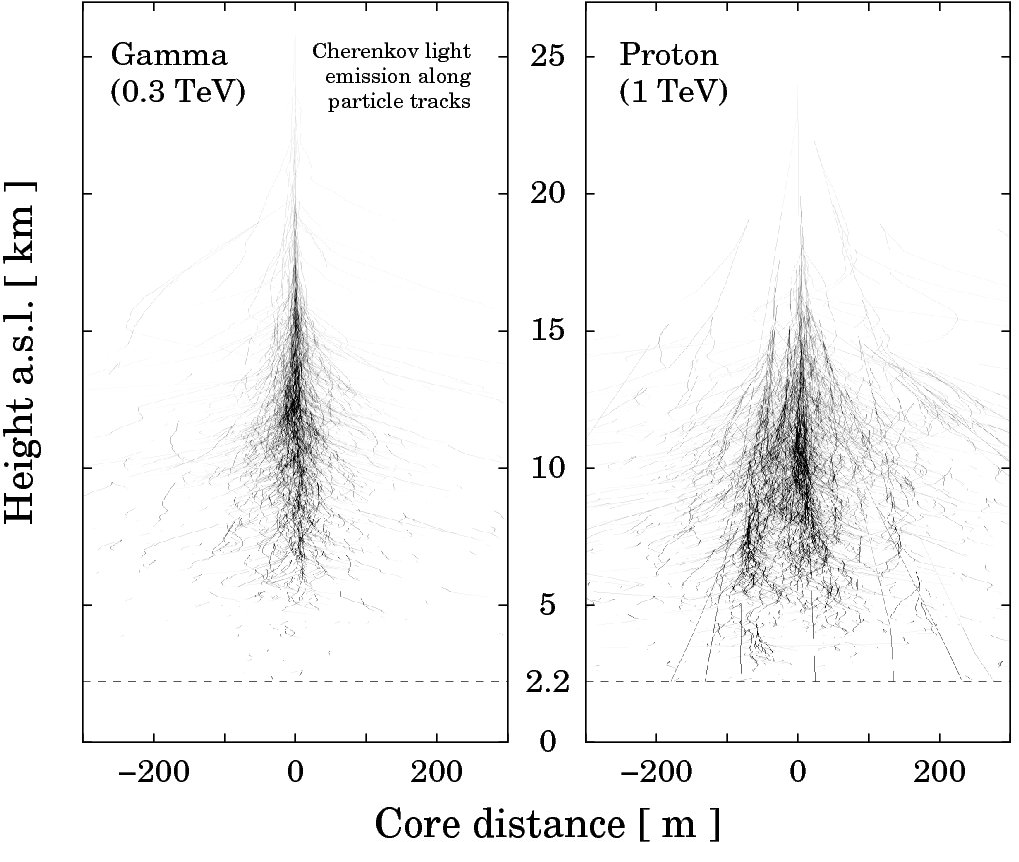
\includegraphics[width=0.7\textwidth]{images/showers_gamma_proton}
    \caption[Gamma Ray and Proton Showers]{
      A gamma ray shower (left) alongside a proton shower (right)~\cite{Bernlohr2008149}.
    }
    \label{fig:gamma_vs_proton_airshower}
  \end{figure}
  
  \FloatBarrier


\cleartooddpage[\thispagestyle{empty}]
\chapter{The VERITAS Observatory}\label{chapter:veritas}

\begin{figure}[ht]
  \centering
  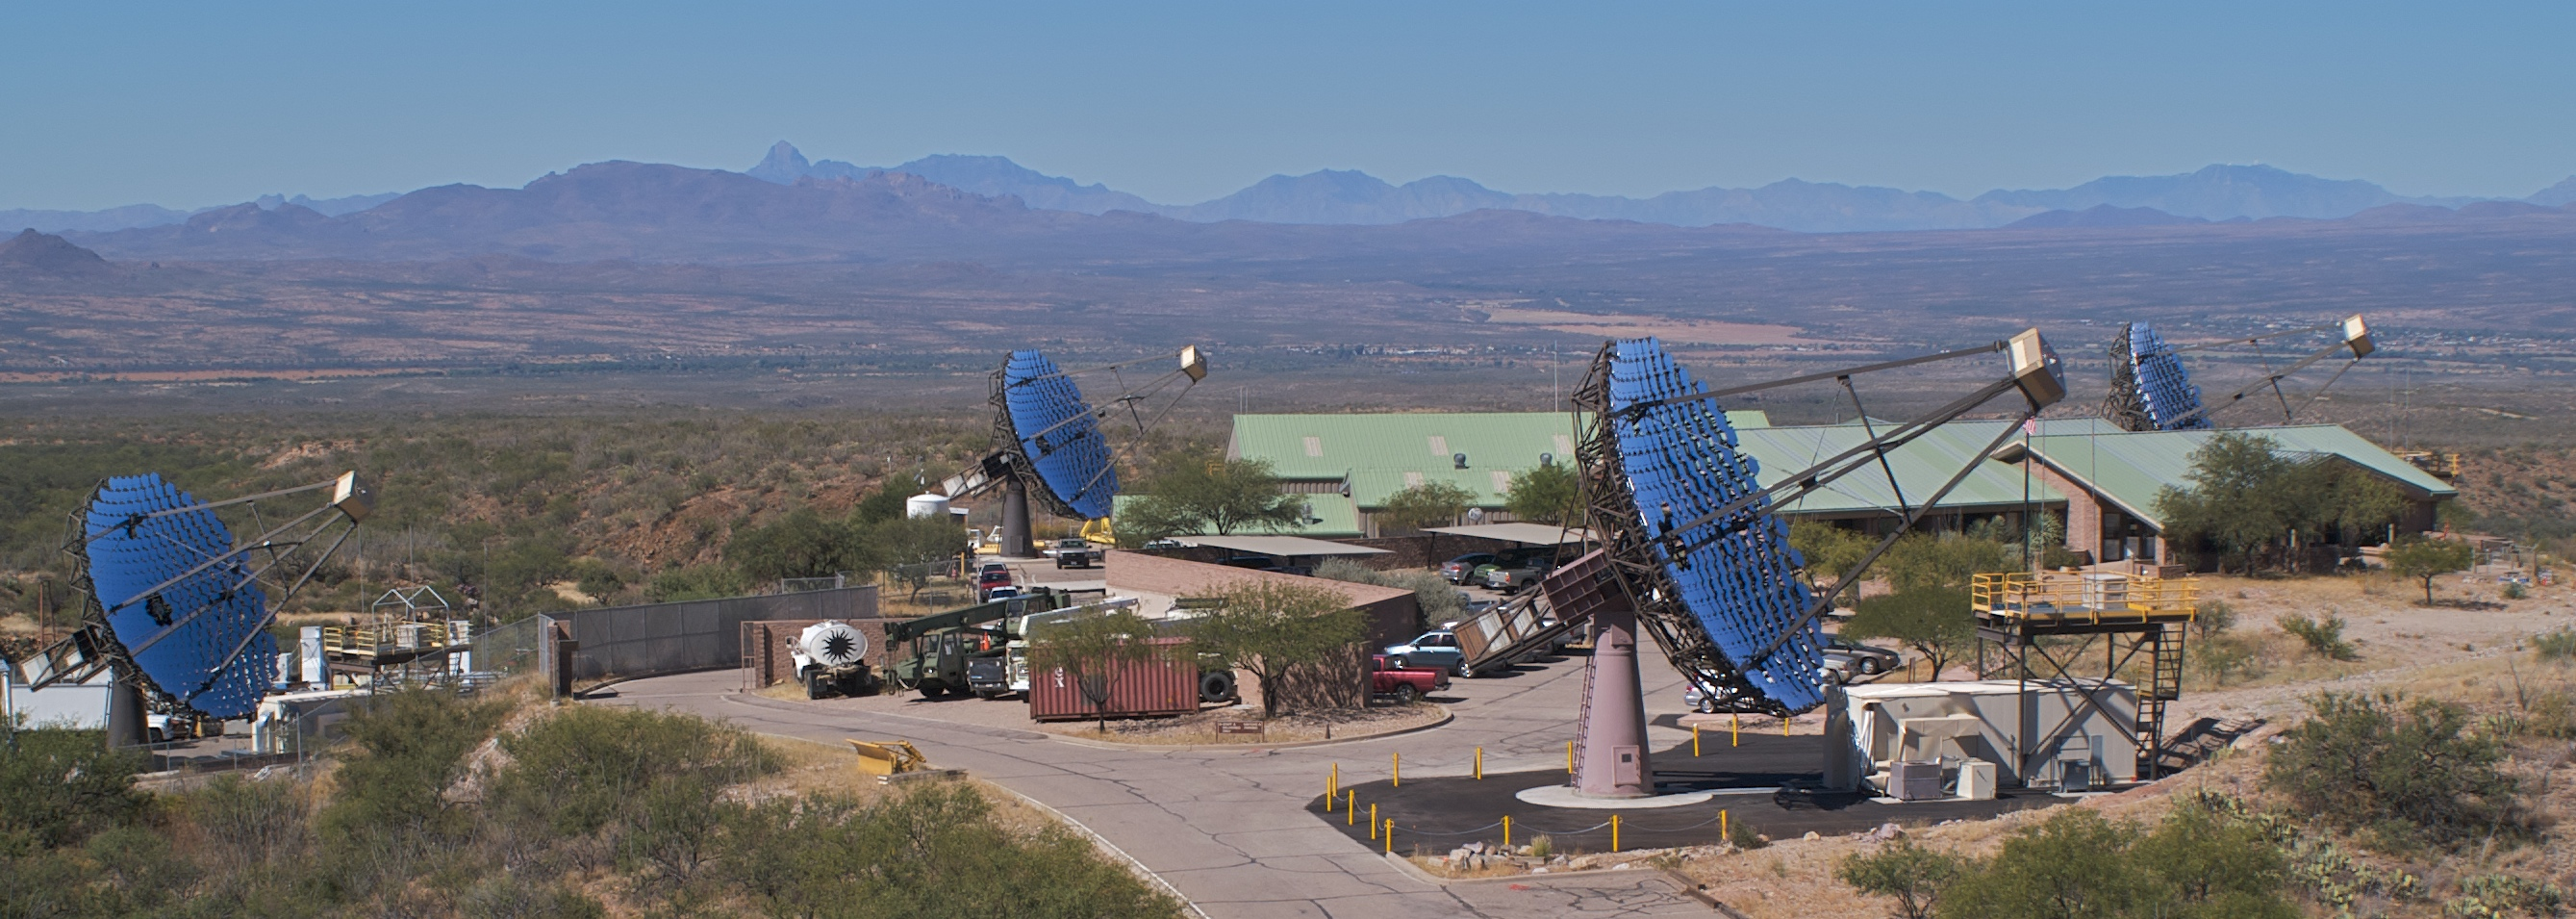
\includegraphics[width=0.95\textwidth]{images/veritas_array_v6}
  \caption[VERITAS Array]{
    The VERITAS observatory.}
  \label{fig:veritasarray}
\end{figure}

VERITAS, or Very Energetic Radiation Imaging Telescope Array System pictured in Figure~\ref{fig:veritasarray}, is a gamma-ray observatory operating in Arizona, USA, and is capable of detecting gamma rays with energies from \SI{100}{\GeV{}} to \SI{70}{\TeV{}}.
The observatory consists of an array of four Imaging Atmospheric Cherenkov Telescopes (IACTs), spaced \nicetilde{}\SI{90}{m} apart.
Each telescope carries an array of 345 mirrors, and a 499 Photomultiplier Tube (PMT) camera on a set of struts.
When a gamma ray produces an air shower in the atmosphere, the shower emits blue-UV Cherenkov photons over a timespan of nanoseconds.
By focusing these photons onto the PMT camera with the mirrors, images of the shower can be taken, in which each pixel of the image consists of analog voltage pulses from each PMT.


In this chapter, the different hardware components are examined, in order of signal propagation.
Section~\ref{sec:telpoint} details Telescope Pointing, including its monitoring and calibration.
The mirrors are discussed in Section~\ref{sec:mirrors}, including their properties and alignment.
In Section~\ref{sec:pmts}, the PMTs are explored, including their performance and calibration.
The trigger system is examined in Section~\ref{sec:trig}, relating how candidate signal voltages are saved while discarding those sourced from noise.
Section~\ref{sec:epochs} discusses the different observatory epochs, as over time, changes and modifications have altered the observatory's performance.


\section{Telescope Pointing}\label{sec:telpoint}

\begin{figure}[ht]
  \centering
  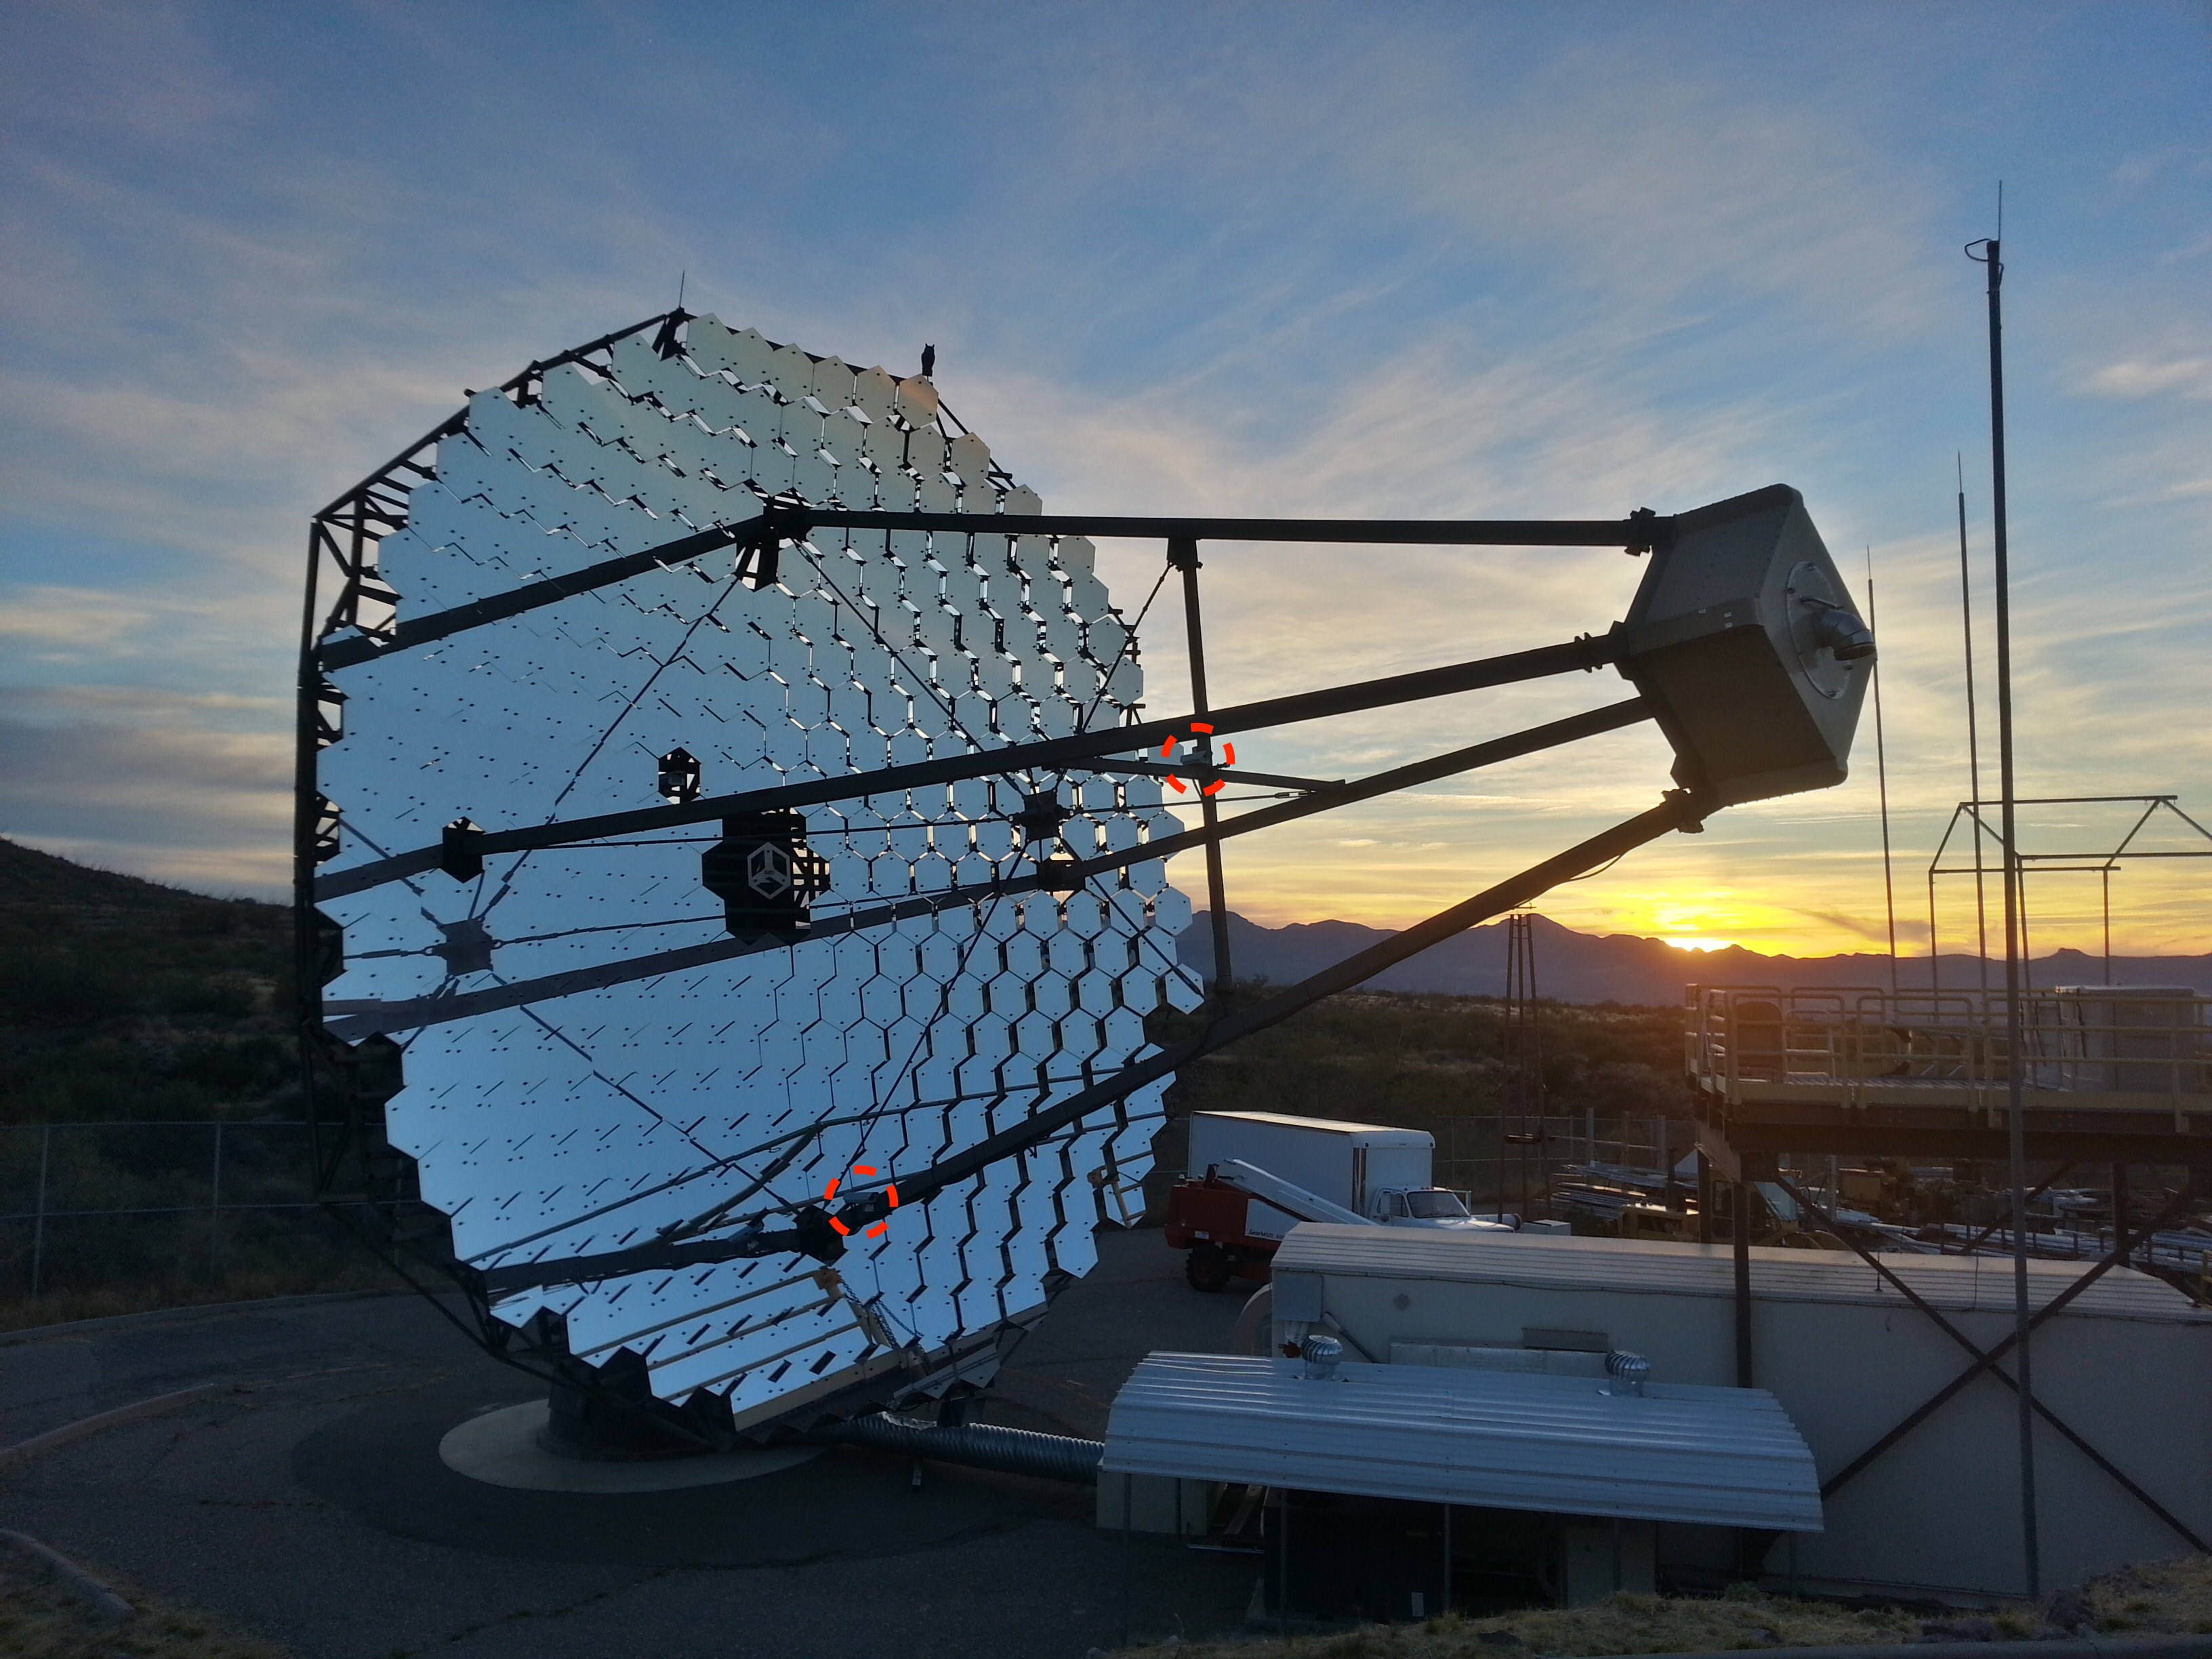
\includegraphics[width=0.95\textwidth]{images/single_telescope}
  \caption[Single Veritas Telescope]{
    View of the 345 mirrors, the camera support structure, and the PMT camera housing at the end of the four supporting arms.}
  \label{fig:davcottel}
\end{figure}

Like most telescopes, each VERITAS telescope has a fixed base and a pointable dish for collecting light.
This dish can rotate in azimuth and in elevation, with enough range in both axes to point at any direction above the horizon that is not blocked by local mountains, though low elevations have reduced gamma-ray sensitivity.
At their fastest, the telescopes slew at a rate of \nicetilde{}\ang{1} per second.
To track where the telescopes are pointing, the motors that drive the azimuth and elevation movement have encoders that digitize the pointing direction of the dishes.
These encoders are attached to the axes of the motors, and thus they are capable of tracking the azimuth and elevation over its entire range of motion.
However, as the dishes are large metal structures, they bend and flex at different elevations and azimuths.
This flexing also experiences hysteresis, where the bending changes whether approaching a pointing target from a higher or lower elevation.
To account for this flexing, the encoder values are then given to a structural model called T-Point, which corrects for the dish structure bending at different azimuths and elevations.
After applying this model, the telescope pointing can be tracked with an accuracy of \nicetilde{}\ang{0.02}~\cite{holder2008status}.
% jeff grube memo http://veritash.sao.arizona.edu:8081/AnalysisAndCalibration/111221_033051/VPM_memo_Dec2011.pdf ?
% or maybe just use https://arxiv.org/pdf/0810.0474.pdf ?

As an improvement to the encoder measurements, a VERITAS Pointing Monitor (VPM) system is also in place.
The VPM consists of two CCD cameras and 4 LED lights affixed to each telescope.
The CCD cameras are oriented such that they can view the PMT camera and the background stars.
The LED lights are attached to the PMT camera, next to the Winston cones detailed in Section~\ref{sec:pmts}.
The first CCD camera is attached below the bottom mirrors, and images the stars in the field of view.
The second CCD camera is attached to the support struts, roughly halfway between the mirrors and the camera, and images the focal plane of the telescope.
Both cameras are marked by red dashed-line circles in Figure~\ref{fig:davcottel}.
During regular observations, these cameras take images of background stars and the focal plane LEDs every two seconds.
By extrapolating the LED positions from the star positions, an improved pointing accuracy of \nicetilde{}\ang{0.007} can be achieved~\cite{VPMmemo}.
%  0.007 comes from Grube 2011 VPM Memo:
%    "VERITAS Pointing Monitor" on https://veritas.sao.arizona.edu/wiki/index.php/VERITAS_Memos
%    20 arcseconds systematic error on VPN calibration (Section 3, last paragraph, and section 5 last paragraph)
%    +5 arcseconds due to scatter of star database positions (Section 5 last paragraph)
%    = 25 arcseconds total VPM systematic error
%
%    25 arcseconds -> 25/3600 -> 0.006944 deg -> rounded to 0.007 deg
This improvement persists down to an elevation of \ang{30}, where the data analysis in this thesis takes place.

\section{Mirrors}\label{sec:mirrors}

When the Cherenkov light from a gamma-ray shower first interacts with the telescope array, it is reflected by some of the 345 mirrors.
These mirrors face towards the incoming Cherenkov light, with the PMT camera facing the mirrors, as shown in Figure~\ref{fig:davcottel}.
When its spherical mirrors, spherical dish, and focal length ratio of \nicetilde{}2 are considered, this configuration is referred to as a Davies-Cotton telescope~\cite{daviescotton}.
Each mirror has an area of \SI{0.322}{m$^2$}, and a spherical curvature radius of \SI{24}{m}.
The mirrors are each mounted along the optical support structure so that the total diameter of the telescope's mirror area is \SI{12}{m}, with a total area of \SI{111}{m$^2$} and a focal length of \SI{12}{m}~\cite{Veritas_Detector}.
Figure~\ref{fig:mirreflect} shows the mirrors' reflectivity as a function of wavelength.
The VERITAS specifications state that the mirror reflectivity must be $\geq 85\%$, between \SIrange{280}{450}{nm}.

\begin{figure}[ht]
  \centering
  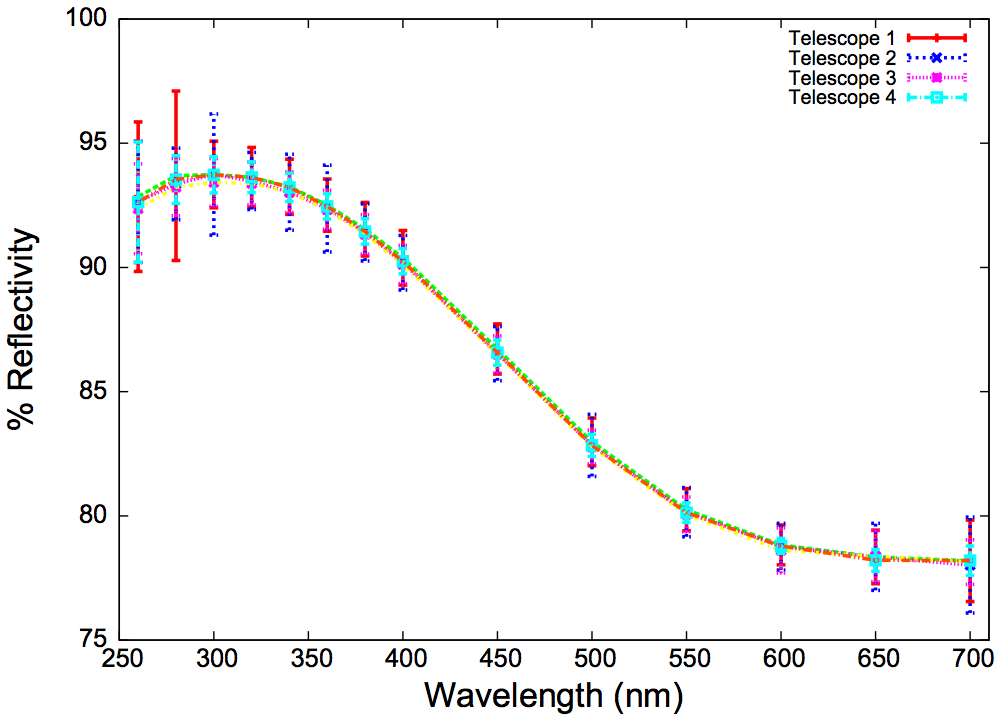
\includegraphics[width=0.75\textwidth]{images/mirror_reflect}
  \caption[Mirror Reflectivity]{
    Mirror reflectivity as a function of wavelength for each telescope, from Ref.~\cite{mirrorfacets}. 
  }
  \label{fig:mirreflect}
\end{figure}

As the mirrors are exposed to the elements, they slowly accumulate dust and scratches.
To combat this, they are cleaned and recoated every two years.
Each mirror is attached to the optical support structure via three adjustable mounting points, allowing for adjustment of the mirror orientation to point directly at the camera, as detailed in~\cite{mirroralign}.
This alignment is measured and adjusted at regular intervals, using background stars as a calibration source.

\subsection{Star Point Spread Function}

Photons that bounce off the mirrors are not reflected perfectly due to the Davies-Cotton design.
This is because of how the mirrors are aligned with the focal point.
When the mirrors' centers are aligned towards a focal point, the edges of these mirrors are inherently not aligned with the focal point~\cite{daviscotton_optical}.
% also see internal VERITAS memo "Optical ray-tracing for VERITAS by Stephen Fega and Vladimir Vassiliev 2005
The result is that a single point-like light source will appear blurred out on the focal plane.
Minor imperfections in the surface of the mirrors, dust, and small mirror misalignments also contribute to this blurring.

This blurring is quantified by a fitted Gaussian function, usually called the Optical Point Spread Function\footnote{Please note that this is different from the PSF described in Chapter \ref{ch:grrecon}, which quantifies the spread in the reconstructed gamma-ray positions.  The OPSF instead describes the spread of UV-Optical photons.} (OPSF).
The OPSF is measured monthly by pointing a telescope at different stars and pointing CCDs at the focal plane.
Figure~\ref{fig:mirrorpolaris} shows a calibration image from the first VERITAS telescope.
The OPSF is roughly gaussian-shaped but with longer tails and a $ \ang{0.06} $ full width half maximum~\cite{Veritas_Detector}.

\begin{figure}[ht]
  \centering
  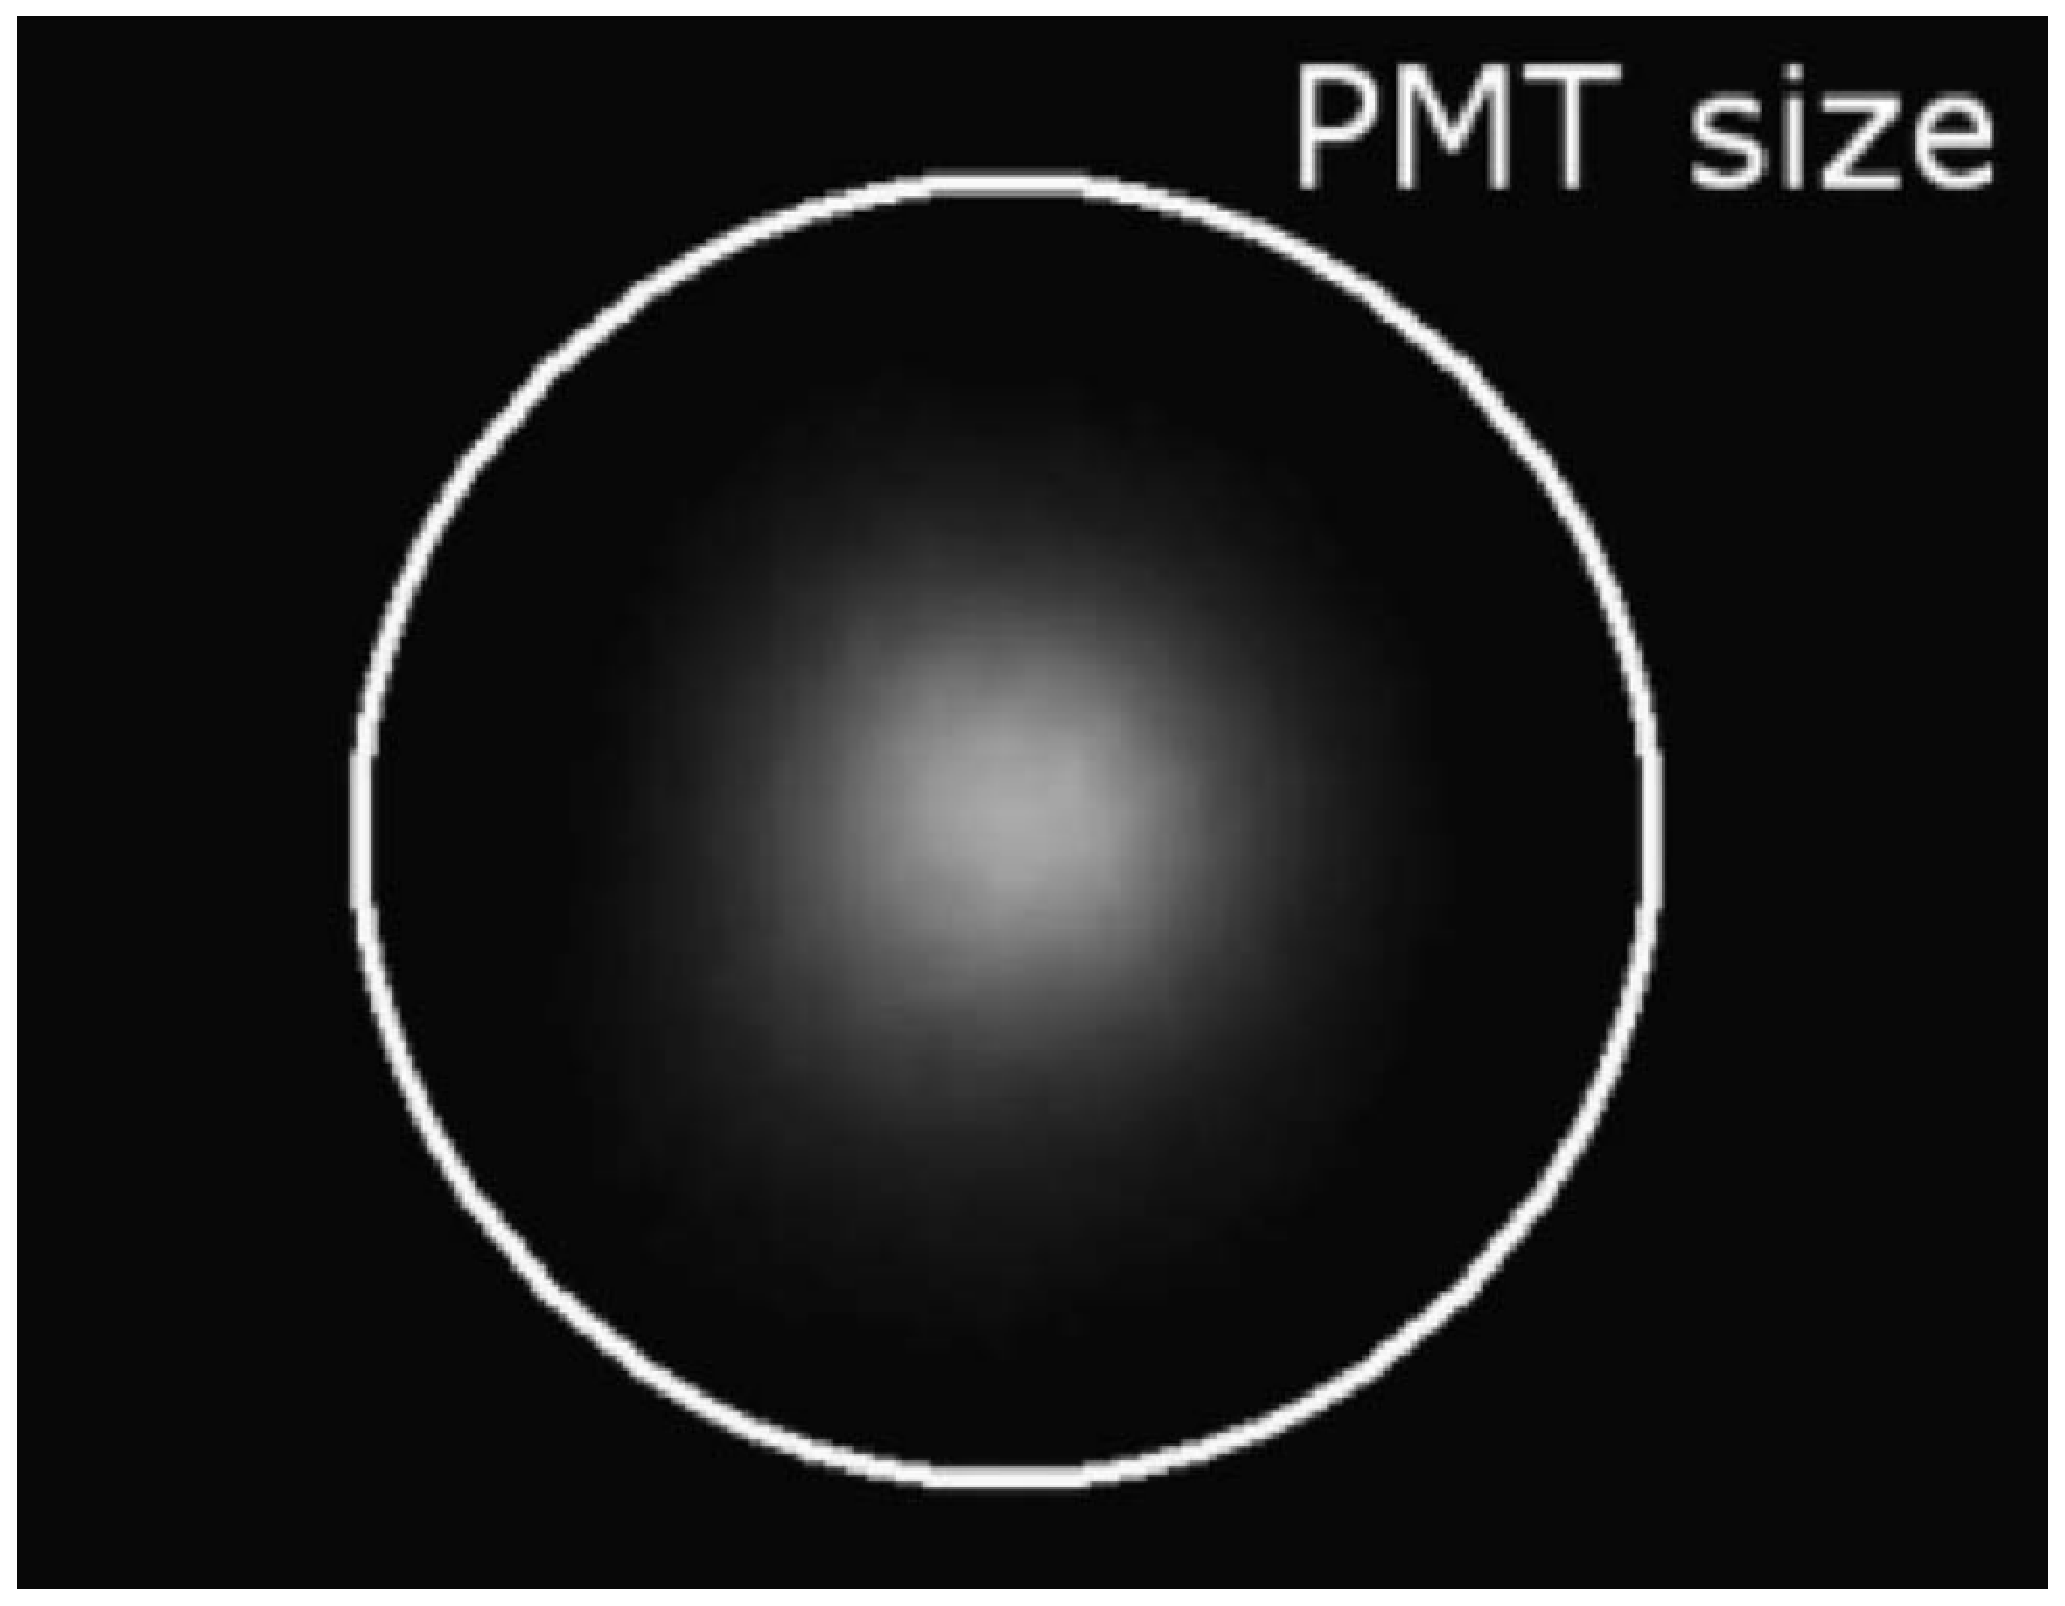
\includegraphics[width=0.75\textwidth]{images/mirror_polaris.eps}
  \caption[Polaris PSF]{
    Image of Polaris after reflecting off the mirrors, demonstrating the shape of the OPSF, from~\cite{Veritas_Detector}.
    The star has a full-width at half-maximum angle of \ang{0.06}.
    The circle indicates the radius of a PMT.}
  \label{fig:mirrorpolaris}
\end{figure}

This point spread function is important, because it determines how accurately Cherenkov showers are imaged.
A larger star point spread function means Cherenkov images are blurred out, which adds to the gamma-ray point spread function, discussed in Chapter~\ref{ch:grrecon}.


\subsection{Mirror Alignment}
% https://veritas.sao.arizona.edu/wiki/index.php/Mirror_Alignment
The mirror alignment procedure is performed by placing a CCD camera at the focal plane, facing towards the mirrors.
The telescope is then pointed towards a magnitude 2 star at \nicetilde{}\ang{70} elevation.
The pointing is known as a ``raster'' scan of the star, where each mirror's field of view is in turn centered on the star.
By using the CCD to examine the position of the star in each mirror, the mirror's alignment can be calculated and corrected.



\section{PMTs}\label{sec:pmts}

Each telescope has a PMT camera on the end of four supporting arms, inside a protective housing.
This camera consists of 499 Photo Multiplier Tubes (PMTs), each with a Winston cone to increase the light collection area for each PMT~\cite{Winston1970}.
% Winston 1970, Hildebrand and Winston 1982, Hildebrand 1985, Welford and Winston 1989
The PMTs are Hamamatsu's model R10560-100-20 MOD~\cite{pmtmodels}.
These Winston cones can be seen attached to the PMTs in Figure~\ref{fig:winstcones}.

\begin{figure}[ht]
  \centering
  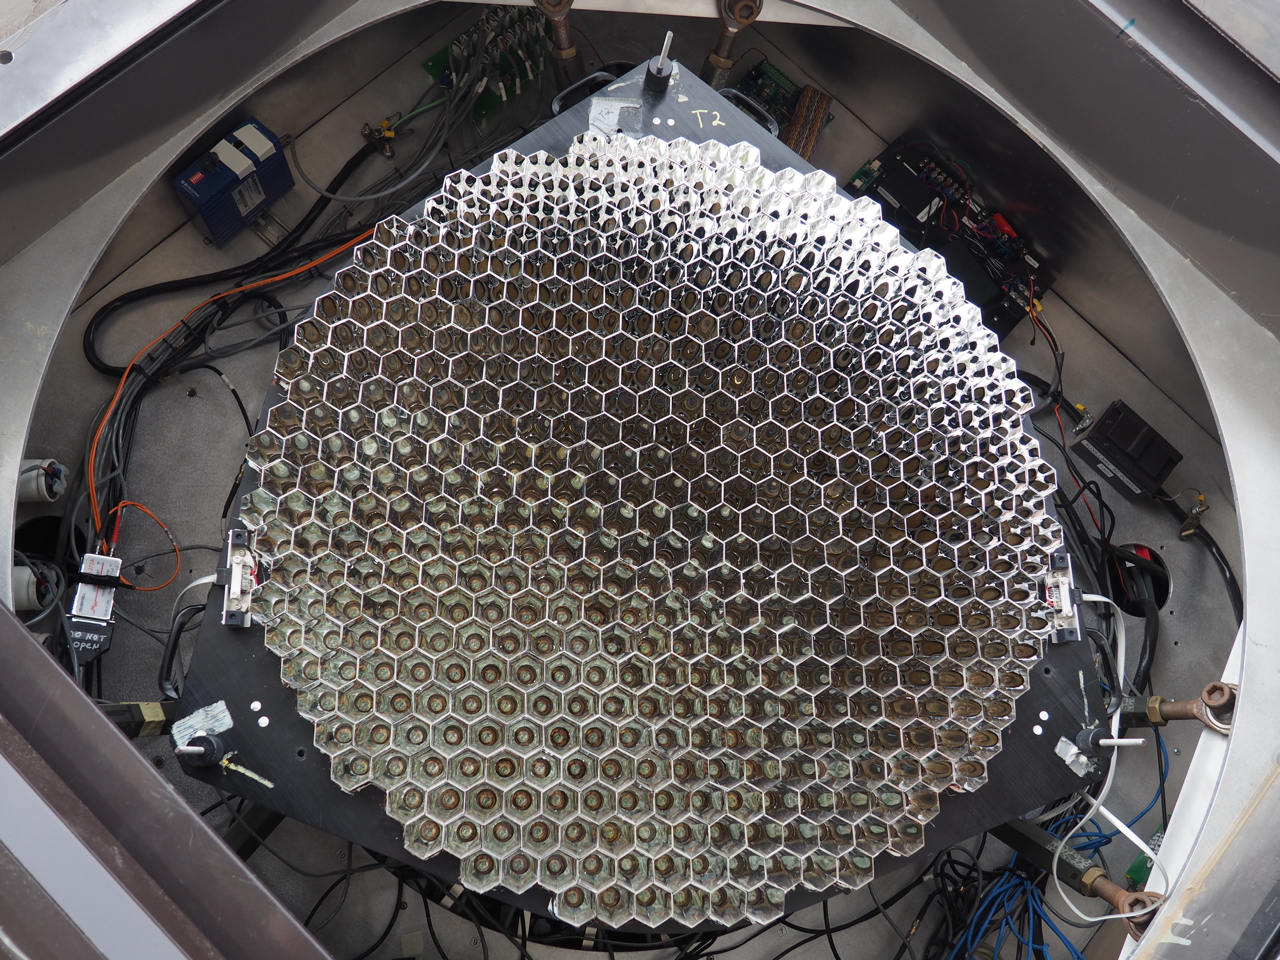
\includegraphics[width=0.75\textwidth]{images/winston_cones_t2}
  \caption[Winston Cones]{
    Hexagonal Winston cones over the circular PMTs, inside the camera housing.
    Image Credit: VERITAS Collaboration.
    \CaptionBlankLine
    }
  \label{fig:winstcones}
\end{figure}


\begin{figure}[ht]
  \centering
  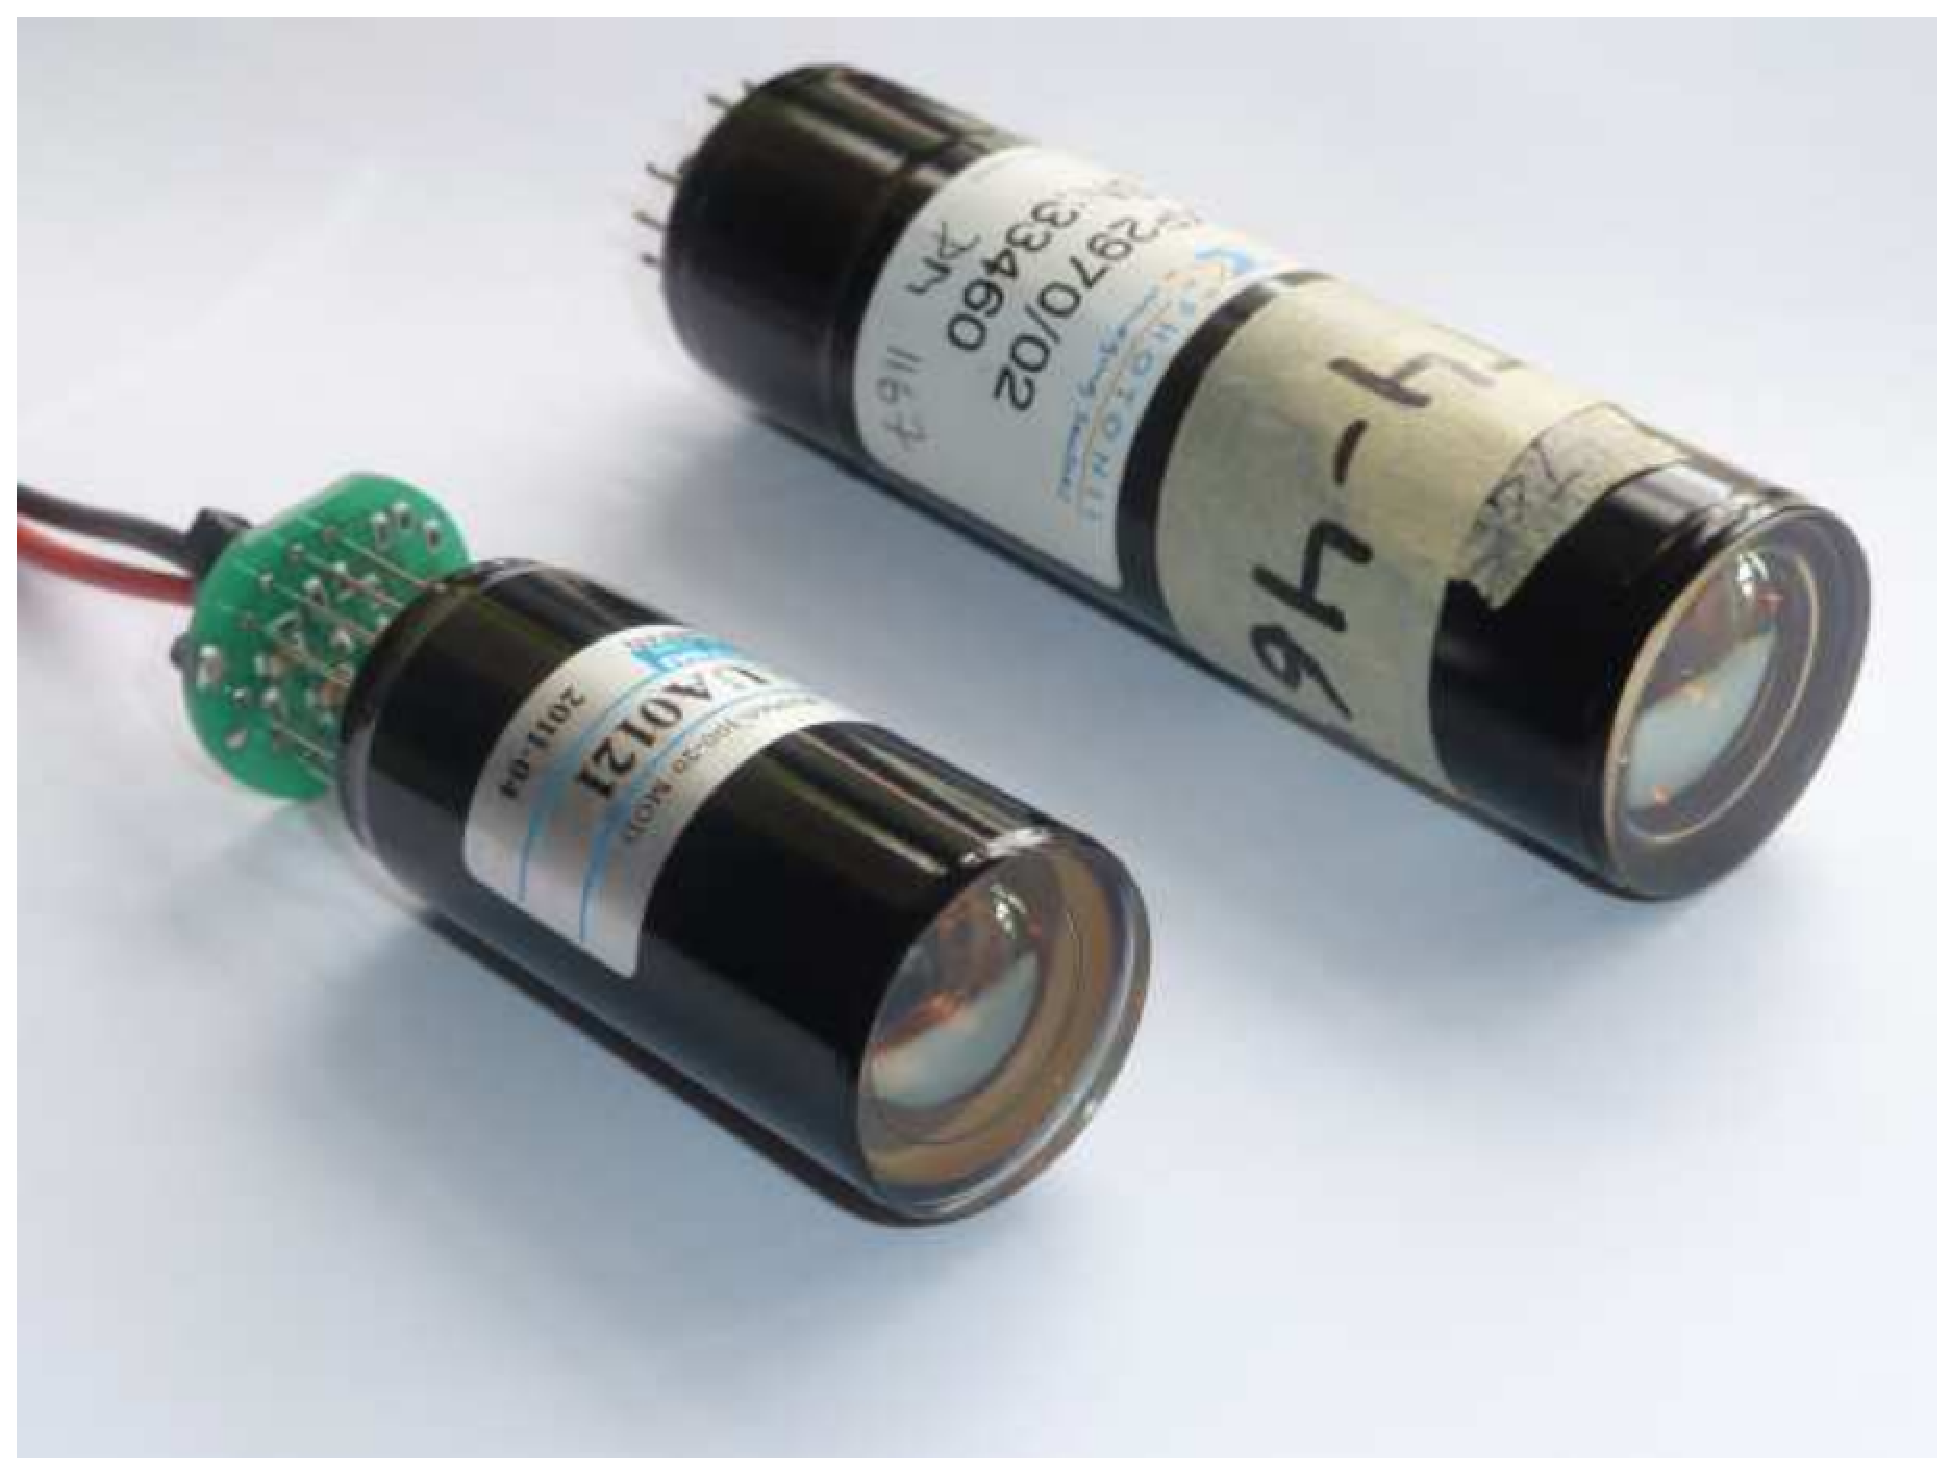
\includegraphics[width=0.75\textwidth]{images/pmt_models/pmt_models}
  \caption[PMT Models]{
    The two PMT models used in the VERITAS cameras~\cite{pmtmodels}.}
  \label{fig:pmtmodels}
\end{figure}

To operate, the PMTs are connected to high voltage, typically \SIrange{900}{1200}{V}.
% mysql -u <username> -h <veritas database> -e "select * from VERITAS.tblHV_Telescope0_Voltages where db_start_time >= '2016-12-01 00:00:00' and db_start_time < '2017-01-30 00:00:00' " >| tmp.txt
% cat tmp.txt | awk '$6>0 {print $6}' | $VERIPY/scripts/hist.py
%
%min      :  275.0
%max      :  1593.0
%mean     :  1054.22
%standev  :  162.73
%elements :  93609
%total    :  98684135.0
%bin width:  131.80
%
%1527 XXX                   6069
%1395 X                      575
%1263 X                     3122
%1131 XXXXXXXXXXXXX        27378
% 999 XXXXXXXXXXXXXXXXXXXX 40171
% 868 XXXXXX               13694
% 736 X                     2437
% 604 X                       14
% 472                      
% 340 X                      149
% mean voltage = 1054, standev = 162, approximate as 1050+-150 = rane of 900-1200
The PMTs' output signals are first sent through an amplifier, before travelling down a \nicetilde{}\SI{40}{m} cable to trigger and digitization electronics stationed near the telescope~\cite{firstVeritas}.

The first circuit that the signal passes through is a Constant Fraction Discriminator (CFD) circuit~\cite{cfd_behavior}.
This circuit's behavior, shown in Figure~\ref{fig:cfd_operation}, duplicates the signal voltage pulse from the PMTs, inverts and delays the duplicate pulse, and adds it back to the original pulse.
This combined pulse is then sent to a Zero Crossing Discriminator (ZCD).
When the input pulse crosses the zero-volts threshold, the ZCD emits a \SI{10}{ns} trigger pulse.
% theres also CFD Design Review Jun 2001: http://www.if.pw.edu.pl/~alice/CFD7.pdf , slide 12

\begin{figure}[ht]
  \centering
  \includegraphics[width=0.95\textwidth]{images/cfd_operation/cfd_operation.pdf}
  \caption[CFD Operation]{
    CFD signal processing, from Ref.~\cite{cfd_operation}.
    An input signal on the left is manipulated to allow for constant fraction discrimination.
  }
  \label{fig:cfd_operation}
\end{figure}

The use of this circuit has two main benefits.
The first is that the CFD circuit will trigger at the same position within the pulse, regardless of the pulse's size.
If a simple voltage-threshold trigger were used instead, the time of the trigger would be earlier for faster-rising large pulses, and later for slower-rising small pulses.
The CFD's zero threshold trigger is invoked when the signal voltage pulse reaches a predetermined fraction of its maximum value.
For VERITAS, this fraction threshold is set at 75\% of its maximum value.
% griffin 2016 thesis, page 47, figure 3.17 caption
The second benefit benefit of this circuit is that when it detects a voltage pulse larger than a given maximum threshold, it can emit an extra logic trigger, called a low-gain trigger.
This extra low-gain trigger is then used by the Flash Analog-to-Digital Circuit (FADC) to switch between high-gain and low-gain mode when digitizing voltage pulses.

Stars and other sources of background light emit background visible photons (Night Sky Background or NSB photons) that can falsely trigger the CFD circuit, contaminating any Cherenkov signals.
In order to reduce this contamination, the CFD circuit is set to ignore any pulses smaller than \SI{45}{mV}.
This threshold is adjusted during observations to account for varying rates of NSB photons.

After the CFD emits a trigger pulse, the signal voltage pulse is passed to the FADC circuit for digitization.
This FADC circuit then, for each 2-nanosecond time bin, measures how large the voltage pulse is with a series of 255 voltage thresholds.
% see Bird 2015 thesis, page 52, top line
% time bin = 2ns, stored in an 8-bit int, so 256 possible values, or 255 values + a 0 value
The highest threshold that is crossed in a single time bin then determines the digital voltage value that is saved to the FADC buffer for that time bin.

{\color{red}(following is not correct: the low-gain FADC signal is always in the signal chain; but delayed by a fixed time offset. When the low-gain switch is set, the readout system simply reads out later -gernot ?? )}
{\color{red}(the fadc puts both high/low gain signals in the same buffer, the high/lowgain bit then decides which time window to read out from that buffer??)}
If the low-gain trigger pulse was also received by the FADC, then the signal is sent to a separate low-gain circuit.
This low-gain circuit does not amplify the signal as much before digitizing it.
The high-gain trigger can only detect signals with at most 120 photoelectrons, while the low-gain trigger can detect signals up to 750 photoelectrons.
This low-gain option increases the digitizable dynamic range of the entire system.
Once the voltage pulse is digitized, it is saved to an \SI{8}{$\mu$s}-long rolling buffer in the FADC, waiting for higher level triggers and signaling the FADC to readout its buffers into a datafile~\cite{Veritas_Detector,veritas_FADC}.

\subsection{PMT Upgrade}
In summer of 2012, all PMTs in the telescopes were replaced with improved PMTs.
Specifically, the original Photonis XP2970 models were replaced with the Hamamatsu R10560-100-20 MOD.
This was done because the R10560 collects 23\% of incident Chernekov photons, 35\% more than the the XP2970.
This higher collection rate means more photons from a shower are detected by the PMT, which makes VERITAS more sensitive to lower energy gamma rays.
In addition, single-photoelectron studies indicate the R10560's voltage pulse's full duration at half maximum time is \nicetilde{}40\% shorter than the XP2970, as shown in Figure~\ref{fig:pmt_pulse_widths}.
These shorter voltage pulses allow for easier discrimination between NSB fluctuations and Cherenkov signals~\cite{pmtmodels}.

\begin{figure}[ht]
  \centering
  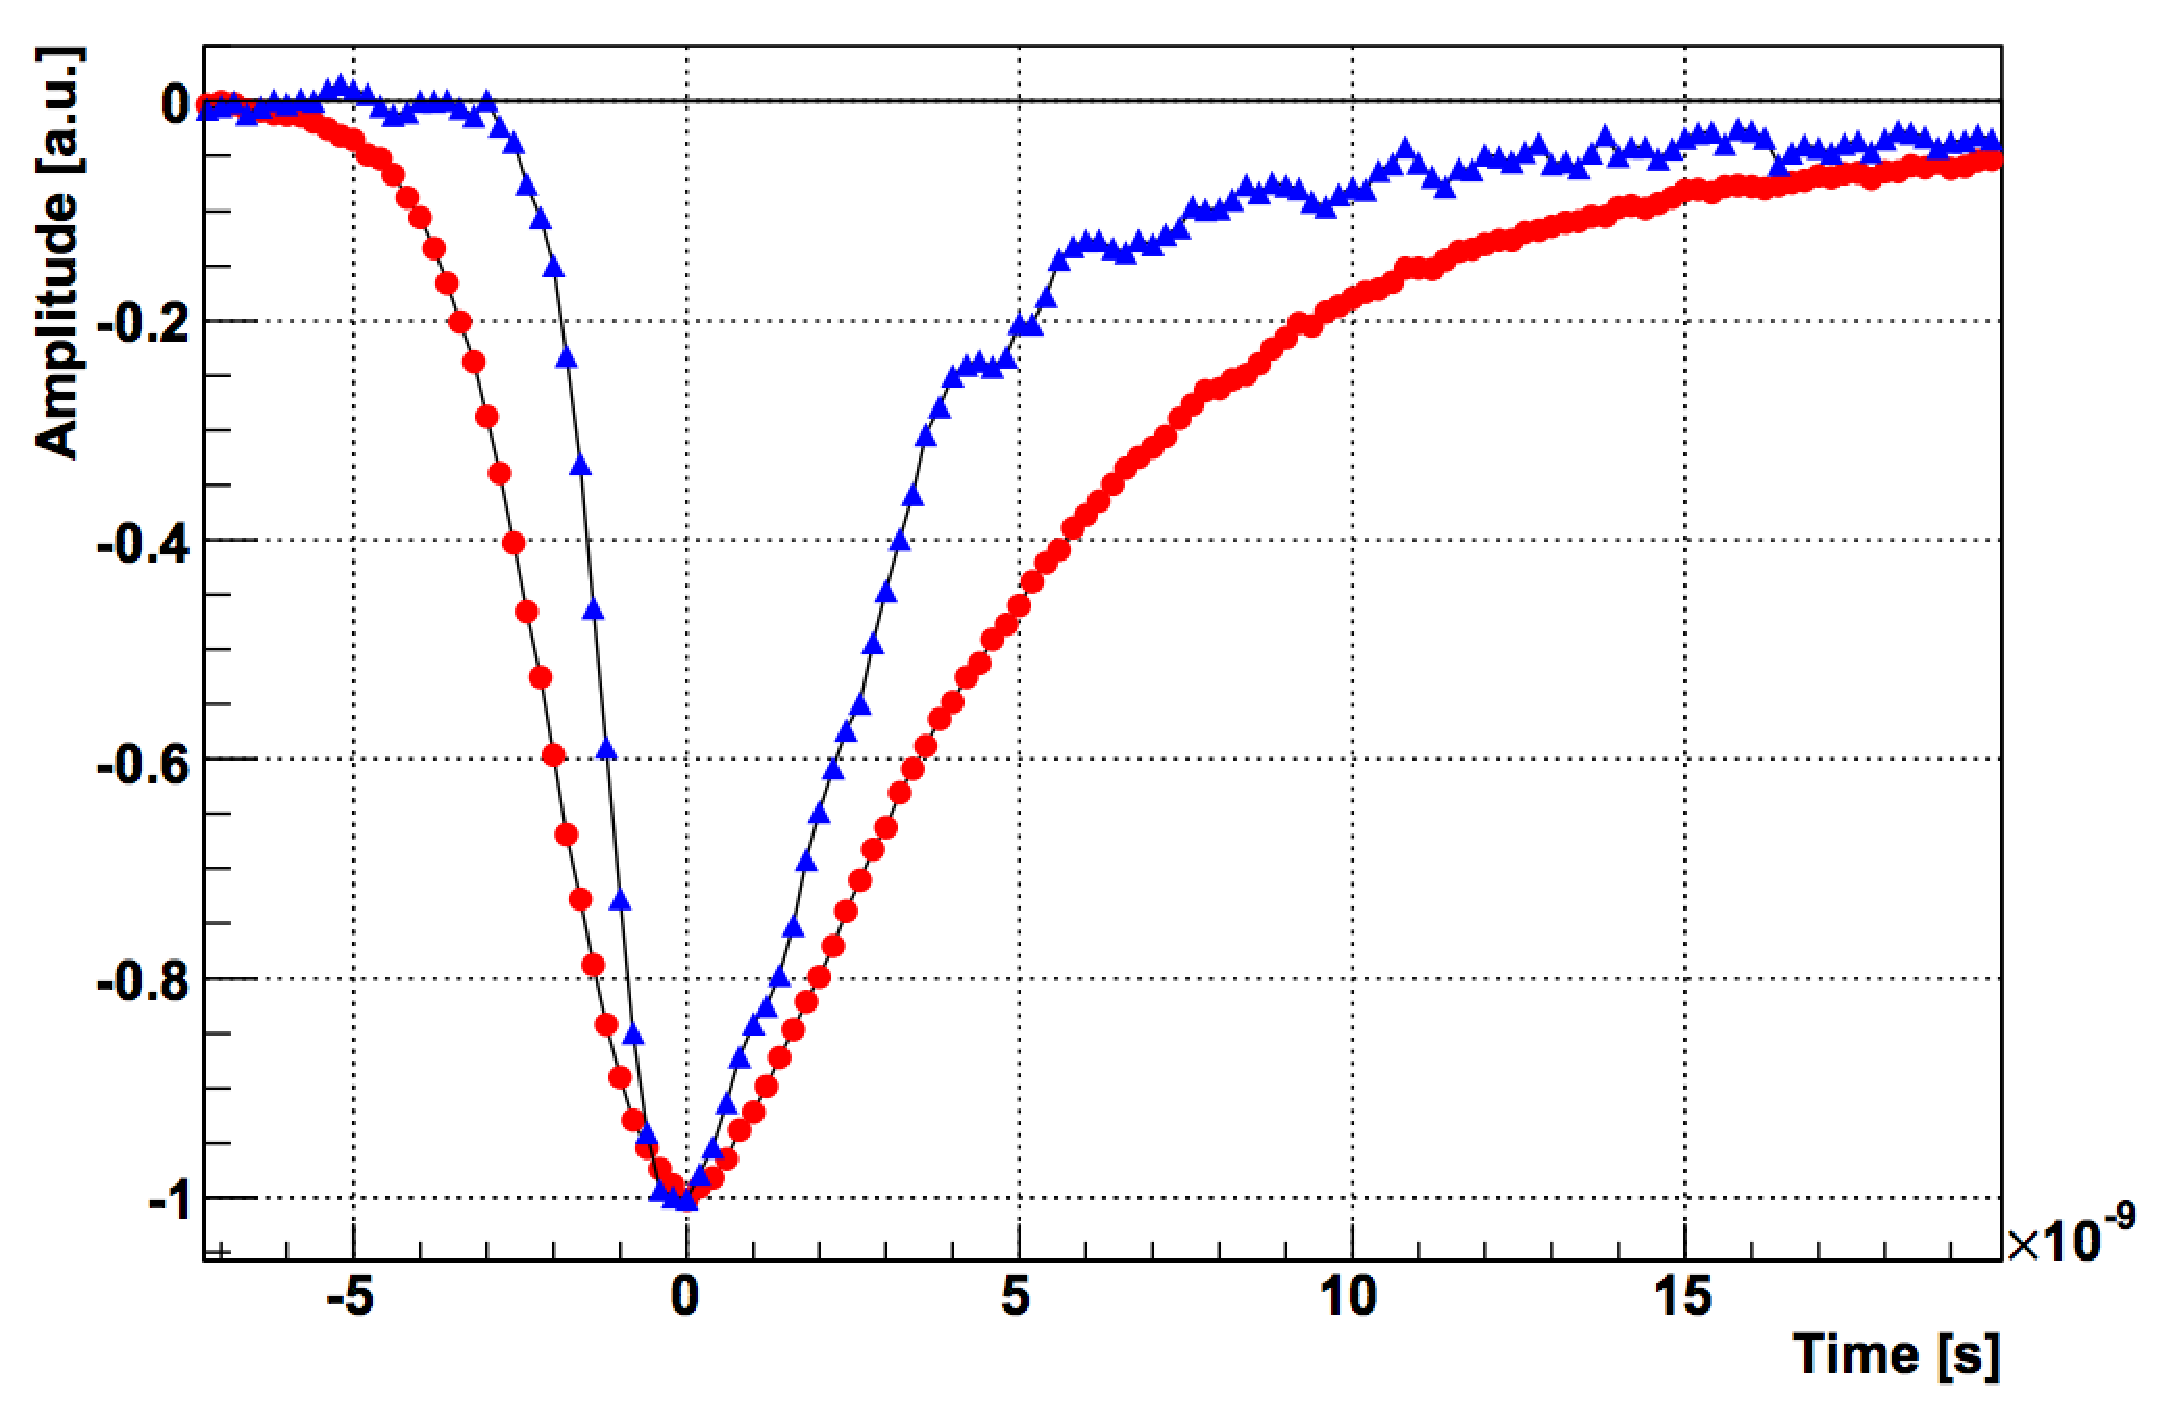
\includegraphics[width=0.75\textwidth]{images/pmt_models/pmt_models_pulsewidths.eps}
  \caption[Pulse Shapes]{
    Pulse shapes of the old XP2970 PMTs (red circles) and the new R10560 PMTs (blue triangles).
    Plots are the average of many afterpulses, normalized to the maximum amplitude.
    Pulses shown include dispersion due to a \nicetilde{}\SI{40}{m} coaxial cable between the PMTs and the digitizer boards.~\cite{pmtmodels}}
  \label{fig:pmt_pulse_widths}
\end{figure}

The data used in this thesis was taken both before and after this upgrade, which means the telescope performance is different for these two time periods.
This is accounted for by separate simulations for each PMT model, mostly resulting in different effective areas (discussed in Section~\ref{subsec:effarea}) at the lower energies.
These epochs are discussed further in Section~\ref{sec:epochs}.


\subsection{PMT Calibration}

While the VERITAS PMTs are all the same model, there are still differences from PMT to PMT that can impact any data taken.
Primarily, these differences can cause the same number of incident photons to create differently-shaped output voltage pulses in each PMT.
To account for these differences, a calibration procedure is applied nightly or semi-nightly.
These are performed with a set of flashing LEDs, placed next to the mirrors such that they illuminate the PMTs.

Once per dark run, the single-photoelectron curves for each PMT are measured.
A dark run is the roughly two-week-long period when the moon is below the horizon at night, providing optimally-dark observation conditions.
This is done by placing an opaque (several-mm-thick metal) plate over the PMTs, with a mm-diameter hole drilled over the location of each PMT.
The LEDs are then flashed repeatedly.
Because the opaque plate has holes drilled over each PMT, each only receives on average \SIrange{0}{5} photons per flash.
Large numbers of flashes can then be used to gather information on each PMT's distribution of pulse widths.
By examining a histogram of the pulses' integrated charges, one can see Poisson-statistic peaks that are formed for integer numbers of photons.
These peaks are then used to translate the integrated charges from the PMTs into their original number of photoelectrons.
These calibration techniques are further detailed in Ref.~\cite{calib_techniques}.


\section{Trigger System}\label{sec:trig}

The operation of VERITAS requires digitizing voltage pulses with voltage samples roughly once per two nanoseconds, per photomultiplier tube.
This means that with 255 voltage levels, 1 second of all voltage measurements would require 1 Terabyte of harddrive space.
Since this is unfeasable with today's computing systems, only subsets of the raw pixel voltages are saved when certain trigger conditions are met.
To complicate matters, photons from atmospheric muons and the night sky background can also cause voltage pulses similar to a gamma-ray shower's Cherenkov photons.
Thus, VERITAS has a system of triggers that reduces the amount of raw data that is saved, while also partially filtering out non-gamma-ray events.

The trigger system consists of three levels.
The L1 is the first and lowest level trigger.
An L1 trigger (sometimes called a pixel trigger) is emitted when a PMT's CFD circuit detects a signal voltage above a given threshold, typically in the 10s of mV.
This threshold voltage is varied throughout data taking by a rate-feedback system, which adjusts the trigger threshold according to the night-sky-background level.

Once L1 triggers have been emitted, they are passed to the L2 trigger system.
The L2 image trigger is emitted when a group of L1 triggers meet two requirements.
The first requirement is that multiple L1 triggers must fall within a certain time window.
Multiple L1 triggers must be within \SIrange{5}{10}{ns} of each other, depending on the VERITAS hardware epoch.
The second requirement is that multiple L1 triggers must all be from neighboring pixels.
More specifically, any pixel with an L1 trigger and two neighboring pixels with L1 triggers (each pixel has 6 neighboring pixels) meets the pattern condition~\cite{veritas_v6_trigger}.
The pattern requirement helps reduce the number of triggers from non-gamma-ray sources.
Night sky background photons are only able to trigger individual pixels, while muons tend to create ring-shaped images.
Once one of these patterns occurs within a time window, the L2 system emits an L2 trigger, which is sent to the L3 array trigger system.

The L3 array trigger system looks for coincident L2 triggers that fall within a \nicetilde\SI{50}{ns} time window.
This window is adjusted for each telescope based on the azimuth and elevation of the pointing, as these can introduce delays between images of up to hundreds of nanoseconds.
During a typical observation period, the L3 trigger rate is around \SIrange{200}{300}{Hz}.
Once an L3 trigger is invoked, a signal is sent to all telescopes that directs the digitized voltages for all pixels in the cameras to be read out from their buffers, and saved to memory.
These pixel voltages can then be processed by the analysis software to reconstruct the gamma-ray events.



\subsection{Deadtime}
When the L3 trigger is invoked and the buffers are being read out, the FADCs are unable to store new PMT voltages in the buffers.
Being unable to store new PMT voltages effectively reduces the amount of time spent observing gamma rays.
This lost time is usually referred to as deadtime.
Since the deadtime is a fixed time loss per event, the percent of time lost due to event readout rises the more frequently events are read out.
For an L3 trigger rate of \nicetilde{}\SI{300}{Hz}, approximately 12\% of the time is lost due to buffer readouts.
Since the L3 rate varies over the course of a single 30 minute run, the deadtime also varies, and is accounted for in the analysis in Chapter~\ref{chapter:analysis}.

\subsection{Time Zero Calibration}
Because all PMTs and signal cables are not identical, there are differences in how long a voltage pulse takes to travel.
More specifically, the time between a) when the photon strikes the PMT's photocathode and b) when the voltage pulse sets off its L1 trigger, can vary from pixel to pixel.
This is usually measured by looking at the average arrival time of many events over all camera pixels.
By looking at the average arrival time, pixels that are consistantly early or late are accounted for, improving image identification.

\section{Epochs}\label{sec:epochs}
Since it was completed in 2007, VERITAS has evolved over several years as collaboration members have upgraded it to improve its performance.
Each improvement in performance needs to be taken into account in the analysis chain.
To organize these different observatory performances, in the data they are referred to as epochs 1, 2, 3, 4, 5, and 6, and are usually denoted as V1, V2, V3, V4, V5, and V6.

The four telescopes were built within a coordinate system where the origin is at 31.675N, 110.962W, the x axis points East, and the y axis points North.
These local coordinates can be described by the format (X n, Y e).
As the first three telescopes were constructed and brought online, data taken after each was considered part of the V1, V2, and V3 epochs.
Telescope 1 was placed at (-37.6n, -23.7e), telescope 2 at (44.1n, -47.7e), and telescope 3 at (29.4n, 60.1e).
In 2007, the fourth telescope was constructed at (-35.9n, 11.3e), and data taken between this point in time and the next major upgrade is considered the V4 epoch.

In September 2009, telescope 1 was moved to a new position (135.4n, -8.61e), after it was demonstrated with simulations that it would grant a \nicetilde{}30\% improvement in sensitivity~\cite{veritas_t1_move}.
Data taken after this relocation is referred to as the V5 epoch.

In August 2012, the PMTs in all cameras were replaced with improved PMTs that had a higher quantum efficiency, improving the telescopes ability to resolve images~\cite{pmtmodels}, and is discussed in Section~\ref{sec:pmts}.
Data taken after this upgrade is considered part of the V6 epoch.

Since these different epochs have different telescope configurations, the instrument response functions are different, meaning each epoch behaves in a quantifiably distinct manner.
For the Dark Matter analysis described in this thesis, only data from the V5 and V6 epochs are used\footnote{This data is detailed further in Table \ref{tab:observation_times}.}.



\cleartooddpage[\thispagestyle{empty}]
\newcommand{\EReco}{$\textrm{E}_{\textrm{Reconstructed}}$}
\newcommand{\ETrue}{$\textrm{E}_{\textrm{True}}$}

\chapter{Gamma Ray Reconstruction Methods}\label{ch:grrecon}

In Chapter \ref{chapter:veritas}, it was explained how the trigger system initializes the readout of PMT voltage traces.
To reconstruct gamma rays, the voltage traces induced by Cherenkov photons must be identified and combined to form an image of the original Cherenkov shower.
Then the shower images from multiple telescopes can be used to reconstruct the original gamma ray's energy and direction.

\section{Pedestal Variation}
  Before reconstructing any events, the pedestal and pedestal variations must be calculated.
  This is done by artificially triggering all pixels once per second during observations, in order to record events that contain only noise.
  The average of the digital counts (dc) of all noise events for each pixel is then the pedestal.
  From this pedestal, the pedestal variations are then calculated for each pixel as the rms of all the dc counts in all noise events, which can be visualized as the distribution of dc around the mean dc.
  In this context, noise events can be due to night-sky-background photons, or from electronic noise.

\section{Pixel Identification}
  The first step is to determine which pixels are part of a shower image.
  This is done by subtracting the dc pedestal from the entire trace, and then summing all trace bins within a fixed window, called the integration length, to get the total dc.

  Most voltage traces have the same general shape: a quickly rising start of the pulse, followed by a longer, slowly falling tail.
  To act as a point of reference in each voltage pulse, the time when the voltage trace is at half of its maximum value is called $T_{0}$.
  The trace is then integrated a second time using a smaller 14 or \SI{24}{ns}-wide time window, starting at $T_0 - 30\%$, to reduce the inclusion of dc from NSB photons and electronic noise.
  This integration is the first of two passes, usually referred to as the double-pass method~\cite{doublepass}.
  If a pixel's first-pass total dc is higher than 5 times the pedestal variation, then it is classified as an image pixel.
  If it is between 2.5 and 5 times the pedestal variation, it is considered a border pixel.

  Once all pixels have been classified, isolated border pixels that have no neighboring image pixel are removed from the image, as they are more likely to be due to noise than Cherenkov photons.
  Then, the time gradient from the image and border pixels can be found by performing a linear fit of the $T_{0}$ times.
  This time gradient can then be used to place a third integration window for a 
with 30\% of the window before each pixel's $T_{0}$, to more accurately measure the charge due to Cherenkov photons in the pixel.
  This third integration window is the second pass in the double-pass method.

  From the image pixels, border pixels, and time gradient, the shower's Hillas parameters~\cite{hillas_params} can be calculated.
  These parameters include the shower size in photoelectrons (or equivalent units), center of charge, angle, length, and width.
  The center of charge is the charge-weighted average of all image and border pixel positions.
  The angle of the shower determines how the image's major axis is oriented in the camera.
  The shower length and width are determined by the rms of the shower image along its major and minor axes, respectively.

\section{Position Reconstruction}\label{subsec:posrecon}
  By examining the images from multiple telescopes, the initial position of the event can be determined.
  This is done by overlapping all telescope images in a single camera coordinate system, and projecting each image's major axis backward in time.
  These axes should intersect very close together, and the average of the intersection points determines the event's initial direction.

  In averaging the intersection points, weighting for each intersection can be applied based on the angle between the two lines.
  This improves the reconstruction, because the intersection point from two images at \ang{90} angles will be less sensitive to image fluctuations than two images at \ang{160}, as shown in Figure~\ref{fig:largeintersectangle}.
  Additionally, the disp method described in Section~\ref{subsec:disp} was explored to provide improvements at lower telescope elevations, though no significant benefit was achieved.

  \begin{figure}[ht]
    \centering
    \includegraphics[width=0.95\textwidth]{images/large_angle_image_intersection_error/laiie_cropped.pdf}
    \caption[Large Image Intersection Angles]{
      In diagram (a), when a noisy pixel is added to an image, the reconstructed position is only moved a small distance (the purple arrow).
      In diagram (b), due to the large angle between images, the error in the reconstructed position is much larger.
    }
    \label{fig:largeintersectangle}
  \end{figure}
  \FloatBarrier

  \subsection{Angular Reconstruction with Boosted Decision Trees}\label{subsec:disp}
    At high elevations, shower images often form small intesection angles, because the telescopes are spread out in two dimensions, relative to the shower in the atmosphere.
    At low elevations near the Galactic Center, however, the telescope array flattens into one dimension, which makes the shower's impact parameter (the shortest distance between the telescope and the shower core axis) smaller for two of the telescopes.
    These two closer telescopes then have very short, almost circular images, which increases the sensitivity of those two image axes to noisy pixels or shower fluctuations, as shown in Figure~\ref{fig:showerhighlowelev}.
    This also causes the remaining telescope images to have large intersection angles, which also reduces the accuracy of the position reconstruction.

    \begin{figure}[ht]
      \centering
      \includegraphics[width=0.75\textwidth]{images/high_elevation_vs_low_shower_images_cropped.eps}
      \caption[Shower Images at High and Low Elevations]{
        In Figure (a), high elevation showers produce long images in all four telescopes.
        In Figure (b), lower elevation showers produce shortened images in two telescopes, and the remaining images form large angle intersection.
      }
      \label{fig:showerhighlowelev}
    \end{figure}

    To better handle these near-parallel image axes at low elevations, the reconstructed position can be determined from more parameters than just the weighted intersection points from the image axes.
    From simulations, the distance between the center of the Hillas shower image and the true position can be calculated, where the angular distance between the two is the \disp{} parameter~\cite{Senturk:2011}, shown in Figure~\ref{fig:dispdiagram}.
    Then, this \disp{} parameter can be provided to a machine learning algorithm~\cite{Beilicke2012NIM}, along with other image parameters like:
    \begin{description}
      \item[\textit{width}:] image angular width
      \item[\textit{length}:] image angular length
      \item[\textit{wol}:] $\frac{\textrm{width}}{\textrm{length}}$
      \item[\textit{size}:] total image dc
      \item[\textit{ntubes}:] number of pixels in the image
      \item[\textit{loss}:] fraction of image pixels at the edge of the camera
      \item[\textit{asym}:] distance between image center-of-dc and the pixel with the highest dc
      \item[\textit{tgrad}:] the slope of the linear time fit to the pixel arrival times
      \item[\textit{cross}:] angular distance between the image center and the average intersection point of the image axes.
    \end{description}
  % list of training parameters: grep "AddVariable" $EVNDISPSYS/src/trainTMVAforAngularReconstruction.cpp
  % how variables are calculated: grep -P "fParGeo.+\=" $EVNDISPSYS/src/VImageParameterCalculation.cpp
  % asym: http://inspirehep.net/record/1395717/files/RdelosReyes.pdf
  % Once trained on these parameters, the machine learning algorithm can construct a boosted decision tree for determining any new image's \textit{disp}, which can then be used with the image axes intersections to improve the gamma-ray reconstructed positions.


    \begin{figure}[ht]
      \centering
      \includegraphics[width=0.5\textwidth]{images/disp_parameter/disp_parameter.pdf}
      \caption[Angular Reconstruction Disp]{
        The \disp{} parameter is the angular distance between the center (red dot) of a Hillas image (blue oval) and the true sky position (green dot).
        Generally, longer shower images have a larger \disp{} angle.
      }
      \label{fig:dispdiagram}
    \end{figure}

    % https://veritas.sao.arizona.edu/wiki/index.php/BDT_Angular_reconstruction
    These parameters for thousands of simulated showers can then be used to train boosted decision trees (BDTs) that estimate the \disp{} for a new shower's images.
    This estimated \disp{} can then be used with the image axes intersection points to more accurately reconstruct the original gamma-ray point of origin.
    
    Once the training is complete, it is tested on a separate set of 17,000 simulated events, which have their true and predicted \disp{}s plotted in Figure~\ref{fig:disptraining}.
    The x axis describes the true \disp{} value for each event, while the y axis describes the \disp{} value estimated by the BDT, with a black $x=y$ line marked, which represents a perfect 1:1 \disp{} reconstruction.
    As events fall on the $x=y$ line, it can be concluded that the BDTs are able to predict the correct \disp{} value for most images.
    {\color{red} You need to be more precise.  You should show also a one dimensional distribution (or various if you want to divide to True DISP bins) and discuss the resolution obtained?? -Orel}

    % made from screenshot of last slide in Dropbox/Presentations/20160719_Group_Meeting.key
    \begin{figure}[ht]
      \centering
      \includegraphics[width=0.85\textwidth]{images/disp_training/disp_training.eps}
      \caption[Disp BDT Training]{
        The true \disp{} vs the BDT-predicted \disp{}, for \nicetilde17,000 gamma-ray event images in T1, from \SI{500}{\GeV} to \SI{200}{\TeV}.
      }
      \label{fig:disptraining}
    \end{figure}
    
    {\color{red} make a profile plot of the true/BDT disp vs true disp, with 68\% containment errorbars, and talk about it in the text! is there a bias? at what disps? }

    The small improvement in the position reconstruction due to the \disp{} method can be seen in Figure~\ref{fig:disp_event_offset}.
    With the Geometric (red) events, more are concentrated further from the point source, while with the \disp{} method, a few more are concentrated at the source itself.
    The limited improvement may be due to the use of boosted decision trees, whereas a previous study with this method utilized a lookup table of six parameters\cite{Beilicke2012NIM}.
    
    {\color{red}Again, you need to be more specific. First, it is important to note this is data, it's always good to ''brag`` that your reconstruction method is tested on data.  Second, you need to discuss the actual resolution obtained with both methods and state the improvement achieved with DISP. I think the RMS might be a better test of this and anyway the mean would be too affected by the tail. In fact I think the quantiles are better?? -Orel}
    
    For the analysis described in Chapter~\ref{chapter:analysis}, the disp method is used when reconstructing gamma-ray events.

    \begin{figure}[ht]
      \centering
      \includegraphics[width=0.85\textwidth]{images/disp_event_offset_hists/dispgeom_comparison.eps}
      \caption[DISP Offset Improvement]{
        The fraction of events at different angular offsets from the Crab and the Galactic Center per solid angle, with Geometric (intersection only) and Disp reconstruction methods.
        Data elevations are the same as in Figure~\ref{fig:datapointingelevations}, while training events were simulated at only \ang{28}.
        {\color{red}(Where is the disp improvement???)}
        {\color{red}(Why is the containment radius worse for disp??)}
        {\color{red}(Redo disp training with 5x events! ??)}
        {\color{red}(change y axis label to Disp/Geometric! ??)}
        {\color{red}(Rerun this histogram for different energies, better to say this had some improvements at some energies or offsets than on average it had no effect.)}
      }
      \label{fig:disp_event_offset}
    \end{figure}
  
  {\color{red}(Find some part of the phase space where DISP offers an improvement, and make plots showing that low energy performance is better, though tradeoff is high energy performance is worse. see https://www.dropbox.com/sh/3w93xgr9g072y2x/AADbIXJZwHFXz40lzslP\_DFVa?dl=0 for the specific plots to remake (??))}
  
  {\color{red}(Also include dispgeom\_comparison\_psftable.crab.png in \$V/thesis/plots , but only focus on my energy range, and switch it to be distributions at each energy)}

  
  \FloatBarrier

\section{Energy Reconstruction}\label{subsec:enrecon}
  To reconstruct the energy of each shower, a lookup table of simulated showers is built.
This database includes the width and length of the shower, how far away its core position is, how bright it was, as well as its reconstructed and true energy.
  By searching through this database for showers that are similar to the one being constructed, then interpolating between shower parameters, the shower's true energy can be reconstructed.


\section{FITS Conversion for Gammalib and CTOOLs}\label{fitsconversion}
  Once gamma rays have been reconstructed with Eventdisplay, they must be exported to Gammalib and CTOOLS~\cite{gammalibctools}.
  This involves converting the event list and instrument response functions (IRFs) to a FITS file format.
  These IRFs consist of the effective areas, the point spread functions, the background models, and the energy dispersion.
  The effective area quantifies the total gamma-ray collection area of the observatory, needed for spectral measurements, and is described in Section~\ref{subsec:effarea}.
  The point spread function (PSF) quantifies the distribution of reconstructed positions for a given true position, which is needed for modeling point sources and extended spatial structures.
  This is described further in Section~\ref{subsec:psf}.
  The background models measure the relative number of observed events in different parts of the camera, and their construction is described in Section~\ref{background_production}.
  The energy dispersion quantifies the distribution of reconstructed energies for a given true energy, and is discussed in Section~\ref{subsec:edisp}.
  
  During the export, several decisions are baked into the event lists and IRFs.
  As this thesis revolves around an analysis at an elevation of \nicetilde{}\ang{30}, the IRFs may rapidly change.
  At this elevation, with VERITAS's field of view of \ang{3.5}, the airmass column density ($g/cm^{2}$) is 20\% higher at the bottom of the camera than at the top.
  Combined with the fact that a observing target can move several degrees over one observation, this means the airmass can change by 10's of percent over a single 30-minute observation.
  This changing atmosphere would mean the IRFs at the beginning of an observation may be measurably different than at the end of an observation.

  To reduce the impact of this, observations are broken up into 8-minute-long parts.
  For each of these 8 minute parts, IRFs are exported alongside the observation.
  A part's average elevation, azimuth, and night sky background rate are used to select the best-matching IRFs for that part.

  \FloatBarrier
  
  \subsection{Effective Area}\label{subsec:effarea}
    % use effective area as a casual noun!
    % plot of effective area vs energy
    Effective area is the measure of how large an observatory's collection area is, which determines how many gamma rays can be detected per unit time, solid angle, and energy.

    For each point in the parameter space, the effective areas are calculated with many {\color{red}(how many?? -Gernot (probably # corsika showers * number of core rescatters * # camera repositions))} Monte Carlo gamma ray simulations.
    This is done in the shower plane, the plane perpendicular to the line drawn between a pointing target and the center of the observatory.
    The effective area is then calculated via:
    $A=\pi R^2 \frac{N_{\text{survived}}}{N_{\text{simulated}}}$
    where R is the radius of the area within which simulated showers are directed to fall, $N_{\text{simulated}}$ is the number of showers that were initially simulated into the area, and $N_{\text{survived}}$ is the number of simulated showers that pass all cuts.
    This effective area is thus a measure of how much detection area the observatory would have if it had a 100\% detection efficiency, which can then be used in calculating a source's flux.
    In Figure~\ref{fig:effarea_paramspace} shows how the effective area peaks to \nicetilde{}\SI{3e5}{m${}^2$} for \SI{3}{\TeV} events at the camera center.

    \begin{figure}[ht]
      \centering
      \includegraphics[width=0.85\textwidth]{images/effarea_plots/effarea_space.pdf}
      \caption[Effective Area Parameter Space]{
        Effective areas at different points in the Energy and Camera Offset parameter space for run 78128.
        Data is shown as the black points, indicating the position of some events from that run in the parameter space.
        The color axis indicates the Effective Area, calculated from simulations, at different gamma-ray energies and distances from the camera center.
      }
      \label{fig:effarea_paramspace}
    \end{figure}

    For the test analyses of the Crab Nebula and the Galactic Center Point Source, the effective areas of all events are shown in Figure~\ref{fig:effarea_usage}.

    \begin{figure}[ht]
      \centering
      \includegraphics[width=0.85\textwidth]{images/effarea_plots/effarea_events.pdf}
      \caption[Effective Areas Used]{
      Illustration of the effective areas used by all events in each analysis.
      From these plots, it is easy to check for events with anomalously high (>\SI{400000}{m${}^2$}) or low (\nicetilde\SI{0}{m${}^2$}) effective areas.
      }
      \label{fig:effarea_usage}
    \end{figure}
  
  \FloatBarrier

  \subsection{Point Spread Function}\label{subsec:psf}

    When reconstructing the source position of each gamma ray, it is necessary to know the uncertainty of the position.
    Primarily, errors in the position come from the randomness of shower images.
    The same gamma ray may develop varying outcomes due to differences in which:
    \begin{itemize}[label=$\bullet$]
      \item particles early in the shower gaining different amounts of energy
      \item angles shower particles scatter at
      \item Cherenkov photons are absorbed by the atmosphere
      \item Cherenkov photons are reflected by the mirrors
      \item Cherenkov photons are converted into PMT photoelectrons
    \end{itemize}
    In the image and position reconstruction, these all means that the same initial gamma ray can develop into a distribution of camera images and reconstructed positions.
    Inversely, a single reconstructed position can come from a distribution of true gamma-ray positions.

    This distribution of reconstructed positions, called the point spread function (PSF), primarily affects the reconstructed shape of gamma-ray emission structures in the sky.
    A singular point source, nominally shaped by a Dirac function, is instead distributed out according to the PSF.
    When searching for an extended source, like a dark matter halo, understanding the distribution of reconstructed positions is important.
    A large PSF on all events, for instance, will artificially expand the observed dark matter halo.

    For VERITAS, the PSF is estimated by simulating many gamma rays, then measuring the distribution of true positions for each reconstructed position.
    The distribution of event positions are fitted with a King function~\cite{king1962} (see Equation~\ref{eqn:king}), as the H.E.S.S. collaboration has noted that the King function better models the longer PSF tails at lower elevations (Section 5.2.2 in Ref. \cite{Mayer2015}).
    The radially-normalized King probability density function is defined as

    \begin{equation} \label{eqn:king}
    \text{PSF}_{king}(r) = \frac{1}{2 \pi \sigma^{2} } \left( 1 - \frac{1}{\gamma} \right) \left( 1 + \frac{ r^{2} }{ 2 \gamma \sigma^{2} } \right)^{-\gamma}
    \end{equation}

    where $r$ is the angular distance from the reconstructed position, $\sigma$ is similar to the width of a gaussian, and $\gamma$ governs how long the tails are.
    A King function fitting algorithm was added to Eventdisplay, that fits the $\gamma$ and $\sigma$ parameters to a set of simulated gamma rays.
    This fits well over almost all of the parameter space.
    In Figure~\ref{fig:psf_paramspace}, the PSF is shown for one Sgr A* run.
    In it, one can see how the PSF containment radius changes vs reconstructed energy and offset from the camera's center.
    Other runs, which have different elevations, azimuths and NSB noise levels will have different values at each point in the energy/offset parameter space.

    % plot of psfs from chunkplot
    \begin{figure}[ht]
      \centering
      \includegraphics[width=0.85\textwidth]{images/psf_king_plots/psf_parameter_space.pdf}
      \caption[PSF Parameter Space]{
        The 68\% containment radius for the Energy/Offset parameter space for Sgr A* run 78128. 
        The green points are from data, showing a subset of the event locations from run 78128 in the parameter space.
        The color axis is the containment radius, calculated from simulations.
        While events from all energies are shown, only events from \SIrange{4}{70}{\TeV} are used (see Section~\ref{sec:crab_analysis}).
      }
      \label{fig:psf_paramspace}
    \end{figure}

    For the Galactic Center and the Crab analyses, the distribution of 68\% containment radii for all events is shown in Figure~\ref{fig:gc_psf_hist}.

    \begin{figure}[ht]
      \centering
      \includegraphics[width=0.85\textwidth]{images/psf_gc_eventhist/eventpsf.pdf}
      \caption[Crab and Galactic Center Event PSFs]{
        The 68\% containment radius for all Galactic Center and Crab Nebula events used in this analysis.
        The odd structure is due to the varying effective area at different offsets and energies, which changes the distribution of events in the PSF table, which already has varying.
        The long tails are likely due to events at the edge of the observable energy and offset ranges, where the PSF gets worse.
      }
      \label{fig:gc_psf_hist}
    \end{figure}
  
  \FloatBarrier
  
  \subsection{Background Models}\label{background_production}
  
    A background model is a 3 dimensional function in camera x (in angle, parallel to azimuth), camera y (in angle, parallel to elevation), and energy.
    Each background model is constructed from one of two templates, and the templates are built from dark run observations (see Figure~\ref{fig:gcfieldsofview}).
    These background models calculate the number of expected events in the camera, per unit solid angle, unit time, and unit energy.
    This is used to quantify how many counts are expected in different parts of the camera when observing any target.
    Understanding the background shape of the camera is crucial for properly studying extended sources, like dark matter halos, which may extend several degrees from the Galactic Center.
    Improperly estimating background models can result in fake structures appearing around an astrophysical target.
    Background models with more than three dimensions are also possible, but require many more simulations, and are beyond the scope of this thesis.
    
    The background models used in this analysis are made from two background templates, one for each of the V5/V6 epochs (see Section~\ref{sec:epochs}).
    The templates are constructed from dark observations, detailed in \ref{veritasdata}.
    Each template is made by binning all background events radially by camera position and by their energy, to produce a spectral function.
    This spectral function can be seen in Figure~\ref{fig:background_profile}.
    The radial function at two different energies is shown in Figure~\ref{fig:background_radial}.

    \begin{figure}[ht]
      \centering
      \includegraphics[width=0.65\textwidth]{images/ctools_background/background_construction.eps}
      \caption[CTOOLS Background Fine Energy Bins]{
        The V5 Background's fine energy bins.
        The top plot shows the number of events in each fine energy bin from all background runs.
        The bottom plot shows the background rate, the number of background events divided by the observation time, solid angle, and energy span.
        The black lines show the background rate in each energy bin, while the blue line shows the used background rate after interpolation is applied.
      }
      \label{fig:background_profile}
    \end{figure}

    \begin{figure}[ht]
      \centering
      \includegraphics[width=0.65\textwidth]{images/ctools_background/radial_profiles.eps}
      \caption[CTOOLS Radial Background Profiles]{
        Radial bin profiles for the V5 background's two large-scale energy bins.
        The blue points are the counts per bin area, while the purple line is a spline interpolation with a 3rd order polynomial.
        The peak and plateau at \ang{0}-\ang{1} is due to the background events not being radially symmetric in the camera, due to the changing atmospheric depth across the camera's field of view.
        For fitting the interpolated curve, the bin values at angles less than \ang{0} and greater than \ang{2.5} are copied from the \ang{0} and \ang{2.5} bins, respectively.
        }
      \label{fig:background_radial}
    \end{figure}
    
    Finally, the spatial and spectral functions $M_{s} \left ( e \right )$ and $M_e \left(x,y,e \right )$ are multiplied together in Equation~\ref{eqn:bck_template}.
    
    \begin{equation}\label{eqn:bck_template}
      f(e,x,y) = A \, \times \, M_{e} \left ( e \right ) \, \times \, M_{s} \left ( x, y, e \right )
    \end{equation} 
    
    The function $f(e,x,a)$ has units of $\frac{\textrm{Number of Counts}}{ \textrm{MeV} \times \textrm{s} \times \textrm{sr} }$.
    The multiplied functions are then scaled with a constant $A$ such that the total integral of the template (integrating across camera x, camera y, and energy) is equal to the original number of counts in the dark runs, as in Equation~\ref{eqn:background_template_function}.
    
    \begin{equation}\label{eqn:background_template_function}
      \textrm{Number of Background Events} = A \, \int \, M_{e} \left ( e \right ) \, \times \, M_{s} \left ( x, y, e \right ) \; dx \: dy \: de
    \end{equation}

    This function $f(e,x,y)$ is the background template in camera x/y, which due to its radial symmetry can then immediatly be used as a CTOOLS background model in RA/Dec.
    Each background template is used in the likelihood analysis as a model multiplied by two free parameters, a normalization factor, and the event energy exponentiated by the spectral index.
    This lets the likelihood fitter scale each run's background model up or down to best match the number of observed events.
    This means the background's absolute value is less important than the relative values in different parts of the camera background or at different energies.
  
  \FloatBarrier

  \subsection{Energy Dispersion}\label{subsec:edisp}
    As events are reconstructed imperfectly, it is important to understand what the distribution of reconstructed energies are for a given true energy.
    This \textit{dispersion in energy} is quantified by an energy migration matrix $E_{i,j}$, where $i$ denotes the $i^{\text{th}}$ reconstructed energy bin, and $j$ denotes the $j^{\text{th}}$ true energy bin.
    The energy migration matrix can be used to account for two significant effects.
    The first is that the reconstruction method introduces biases in the event energy, meaning an event at a given true energy can be reconstructed on average at a higher or lower energy.
    The second effect that is accounted for is the dispersion in the reconstructed energies.
    Gamma rays with the same energy will have their energies reconstructed as a distribution close to the true energy.
    These fluctuations can be due to randomness in air shower development or atmospheric absorption of Cherenkov photons.
    This has the effect of distributing events in each energy bin of a spectra.
    In the gamma-ray spectra of astrophysical sources, which often follow a power law, lower energy bins tend to have more events than higher energy bins.
    This results in lower-energy dispersion contributing more to the higher-energy bins than the higher-energy dispersion contributes to the lower-energy bins.
    When not accounted for, this has the effect that the energy dispersion will harden observed astrophysical spectra.
    In Figure~\ref{fig:migmatrix}, a migration matrix is shown.

    \begin{figure}[ht]
      \centering
      \includegraphics[width=0.85\textwidth]{images/edisp_plots/edisp.pdf}
      \caption[Energy Migration Matrix]{
        An energy migration matrix used with Sgr A* run 82288.
        The reconstructed energy is on the x axis, and the true energy is on the y axis.
        The z (color) axis denotes the number of simulated events that passed all cuts.
        Events at a given \ETrue{} are reconstructed at a spread of \EReco{}.
        This spread is due to the variability in how air showers develop in the atmosphere.
        Small variations early in the shower can have a large impact on the shower's cherenkov image, meaning the shower can look like it was from a higher- or lower-energy gamma ray.
        At the lowest \ETrue{} energies, events are reconstructed at higher \EReco{} energies.
        This is due to ??.
        
        {\color{red}Need to explain downturn at lowest energies?? -Gernot}
        {\color{red}Explain that downturn is probably due to edge effect, where the large population of true  low energy events have more that fluctuate to higher energies, and get reconstructed at higher energies.  ??}
        {\color{red}(add grey region describing energies used in analysis (4-70 TeV)   ??)}
        {\color{red}Again, please describe in the text non-trivial features in the plot (the bias at low energy) ?? -orel}
        {\color{red}Add boundary lines in reconstructed energy based on event cuts??}
        {\color{red}Check other thesis for energy migration matrix stuff and explainations??}
        {\color{red}Check how anasum low-energy limit is calculated, and where it is applied??}
      }
      \label{fig:migmatrix}
    \end{figure}
  
  \FloatBarrier

\section{Camera Studies}
  The objective of this thesis is search for dark matter via the existence of a gamma-ray halo that is both extended and faint.
  The extension and faintness of the halo, plus the relativly large amount of noise near the Galactic Center, make it a priority for understanding how the VERITAS camera behaves in high-noise conditions.
  In order to better understand the camera's behavior in the reconstruction method, several studies were performed.

  \subsection{Background Structure at the Low Energy Threshold}\label{subsec:bkgstructure}
    To produce background models, events were binned according to their energy, elevation, and camera x and y coordinates.
    As a result of this detailed binning, some new effects were noted.
    First, a series of gamma-like events were selected from observations with no known gamma-ray sources.
    These events were then divided into equal-statistics energy bins.
    For each bin, all the contained events were then binned in camera x and y.

    For a set of high-elevation observations, these backgrounds are shown in Figure~\ref{fig:back_highelev}.
    It can be seen that all events are divided up into 3 equal-statistics energy bins in Figure~\ref{fig:back_highelev}.A.
    Each energy bin is then binned in camera x and y in Figures \ref{fig:back_highelev} B, C, and D.
    At these high elevations, the distribution of events in each energy bin is radially symmetric about the camera center.
    This happens because the gamma ray's point of origin, and its shower image in the camera, are usually several tenths of a degree away from each other.
    In addition, the atmospheric column density is similar in all parts of the camera.
    However, structures start to break the radial symmetry at low energies and elevations.
    The cause of these structures is explored in Section~\ref{subsubsec:diffusesims}.

    \begin{figure}[ht]
      \centering
      \includegraphics[width=\textwidth]{images/ctools/backgrounds_highelev.eps}
      \caption[FITS Background at \ang{50} Elevation]{
        Gamma-like events from 52 observations (approximately \nicetilde20 hours) of M82, between \ang{50} and \ang{52} elevations.
        Events in Figure A are divided into 3 equal-statistics energy bins, and binned in Camera Coordinates in Figures B, C, and D.
        Notice the left-most bin (2\%-34\%) overlaps the histogram peak (at -0.5) in the energy histogram by \nicetilde 30\% of its width, unlike in Figure~\ref{fig:back_lowelev29}.
      }
      \label{fig:back_highelev}
    \end{figure}

    In Figures \ref{fig:back_lowelev29} and \ref{fig:back_lowelev26}, the same plots are constructed for a set of low-elevation (\nicetilde{}\ang{29} and \nicetilde{}\ang{26} respectivly) observations, using dark observations.
    See Section~\ref{background_production}, Figure~\ref{fig:gcfieldsofview}, and Section~\ref{sec:bkgmodels} for more discussion.
    It can be seen that in different energy bins, the background possesses different shapes.

    \begin{figure}[ht]
      \centering
      \includegraphics[width=\textwidth]{images/ctools/backgrounds_lowelev29.eps}
      \caption[CTOOLS Background at \ang{29} Elevation]{
        15 Sagittarius A* Off runs (\nicetilde7.5 observation hours), between elevations $ \ang{27.5} $ and $ \ang{30} $.
        Events are divided into 6 equal-statistics energy bins, of which four are binned in Camera Coordinates in Figures B, C, D, and E.
        Notice the left-most bin (from 2\% to 17\%) does not overlap the peak (at $\textrm{log}_{10}\left ( \textrm{TeV} \right ) \approx 0.3$, unlike in Figure~\ref{fig:back_highelev}.
      }
      \label{fig:back_lowelev29}
    \end{figure}

    \begin{figure}[ht]
      \centering
      \includegraphics[width=\textwidth]{images/ctools/backgrounds_lowelev26.eps}
      \caption[CTOOLS Background at \ang{26} Elevation]{
        10 Sagittarius A* Off runs (\nicetilde5 observation hours), between elevations \ang{24} and \ang{27.5}. 
      }
      \label{fig:back_lowelev26}
    \end{figure}
  
  These effects are also noticeable in the galactic (l,b) event maps.
  In Figure~\ref{fig:bkgvsel_crab}, the top plot shows the positions of all events.
  The middle histogram shows the distribution of event energies, and the bottom plot shows the positions of events in a limited energy range, \SIrange{1.5}{3.25}{\TeV}.
  The middle plot demonstrates that, as event energy decreases, fewer events are detected.
  When events in this limited energy range are plotted in the bottom plot, a faint deficit appears along the bottom of the camera.
  This faint deficit is due to the \nicetilde20\% higher column density at the low-elevation parts of the camera.
  This higher column density causes air showers to start farther away from the telescopes, where more Cherenkov photons are absorbed, resulting in fewer events being detectable in the lower half of the camera.

  When similar plots are made for the Galactic Center in Figure~\ref{fig:bkgvsel_sgra}, the effect is much stronger, and rotated.
  In the top plot, events are radially symmetric around the source position.
  When only the events from \SIrange{1.5}{3.25}{\TeV} are plotted, a much clearer deficit is visible on the lower right part of the plot.
  This area corresponds to the deficit at the bottom of the camera in Figures \ref{fig:back_lowelev29}.B and \ref{fig:back_lowelev26}.B.
  This rotation occurs when converting between camera x/y coordinates (Earth Elevation/Azimuth) and Galactic coordinates (l,b).
  The degree of rotation also changes throughout individual runs, which further blurs this effect.
  For the Crab plots in Figure~\ref{fig:bkgvsel_crab}, the rotation is only a few degrees, while for Sgr A* in Figure~\ref{fig:bkgvsel_sgra}, it is closer to \ang{70}.
  
  This effect is important to the analysis because it implies that, at the lowest energies, the background rate is not radially symmetric.
  Radial backgrounds (sometimes referred to as acceptances) are typically used in VERITAS, as no other camera x/y or energy dependence had been demonstrated until now.
  As the analysis in this thesis only has a few hours of background observations (see Table \ref{tab:observation_times}), only radially symmetric background templates and models could be constructed, which then required limiting the final analysis to $\geq\SI{4}{\TeV}$.
  
  \begin{figure}[ht]
    \centering
    \includegraphics[height=0.9\textheight]{images/background_vs_elevation/background_vs_elevation_srccrab.eps}
    \caption[Background Vs Elevation Crab]
    {\small 
      Plots of Crab Nebula observations.
      Top: Skymap of all events.
      Middle: Histogram of all events in energy.
      Bottom: Skymap of events from \SIrange{1.5}{3.25}{\TeV}.  
      The blue circles centered on the Crab Nebula highlight the radial symmetry of the top plot, and the lack of radial symmetry in the bottom plot.
    }
    \label{fig:bkgvsel_crab}
  \end{figure}

  \begin{figure}[ht]
    \centering
    \includegraphics[height=0.9\textheight]{images/background_vs_elevation/background_vs_elevation_srcsgra.eps}
    \caption[Background Vs Elevation Sgr A*]
    {\small 
      Plots of Sgr A* observations.
      Top: Skymap of all events.
      Middle: Histogram of all event energies.
      Bottom: Skymap of events from \SIrange{1.5}{3.25}{\TeV}.  
      The blue circles centered on the Galactic Center highlight the radial symmetry of the top plot, and the lack of radial symmetry in the bottom plot.
    }
    \label{fig:bkgvsel_sgra}
  \end{figure}
  
  \FloatBarrier

  \subsection{Diffuse Simulations}\label{subsubsec:diffusesims}
    Diffuse simulations were performed at similar energies and elevations to see if this effect was still present.
    These consisted of simulating 50,000 gamma rays with CORSIKA~\cite{corsika1998} at 1.4, 1.6, 2, and \SI{5}{\TeV}.
    The telescopes were fixed to an (azimuth,elevation) of (\ang{193}, \ang{28}).
    The events themselves were distributed in a diffuse \ang{2.5}-radius disk.
    To approximate a simple gamma-hadron cut, any events with a mean-scaled-width falling outside the range of -2.0 to 0.5 were removed, which eliminates many of the showers that appear proton-like.
    These remaining 'gamma-like' events are then binned in camera coordinates in Figure~\ref{fig:back_simdiffuse}.

    \begin{figure}[ht]
      \centering
      \includegraphics[width=\textwidth]{images/backgrounds_diffuse_vs_data/backgrounds_sims/backgrounds_sims.eps}
      \caption[Diffuse Simulated Backgrounds]{
        Diffuse simulated gamma-like events in the camera coordinate system at a \ang{28} elevation, at 4 different initial energies.
        {\color{red}is this true or reconstructed positions??}
      }
      \label{fig:back_simdiffuse}
    \end{figure}

    The ring and crescent structures persist in these diffuse simulations, implying these are physical effects of the atmosphere and camera, rather than a problem with the reconstruction method.
    {\color{red}(But what is the effect? I remember Gernot mentioning something about an edge effect? You should explain it here. --Orel??)}
    {\color{red}(The top-of-camera vs bottom-of-camera differences are due to the atmosphere, but I'm not sure what causes the deficit in the middle at the lower energies... ??)}
    {\color{red}(I am not sure what is the reason for the deficit in the middle. Are simulations always with a wobble? Maybe the showers are very small and always at some distance from the centre of the camera?? -Orel)}
    {\color{red}(Consider playing with the distribution of disps and the radial areas??)}

    This striking effect can be seen in the Galactic Center data in Figure~\ref{fig:bkgvsel_sgra}.
    These structures, and their strong dependency on both the energy and elevation of the telescopes may be a large factor in why the low-energy threshold regime of gamma-ray telescopes is poorly understood.
    Incorporating this effect into the instrument response functions would require creating another batch of diffuse simulations with elevation increments smaller than \ang{5}, and calculating instrument IRFs at these finer elevation increments, and at different camera x, camera y, and energy points in the parameter space, all of which are computationally expensive.
    An alternative solution might be to assemble templates for the camera backgrounds.
    These templates can utilize observations at different elevations to quantify how the template shape changes, and can be built for custom time windows, including accounting for the effects of stars and disabled pixels, which are discussed in the next subsection.
    However, due to time constraints these templates were not constructed.
    
    A secondary effect of the previously mentioned diffuse simulations may be that the effective area and energy dispersion IRFs may become more accurate.
    Currently, IRFs are calculated by simulating gamma rays in the atmosphere at a single elevation and azimuth, and then wobbling the cameras away from these events by a fixed angle $W$, typically from \SIrange{0.25}{2.0}\degree.
    This wobbling is done randomly, to sample various parts of the camera evenly.
    This means that the calculated effective area and energy dispersion are averages over a ring of radius $W$ around the camera center.
    The above affect in the previous paragraphs shows that at a fixed elevation, different parts of the camera possess different background rates.
    This implies that the effective areas of the background protons and electrons change with respect to camera x and camera y.
    Since this is an effect of the atmosphere's changing depth, it hints that the \textit{gamma-ray} effective areas also change with respect to camera x and camera y.
    And, since different parts of the camera are sensitive to different energies (due to the changing atmosphere), using diffuse simulations in different parts of the camera may improve the accuracy energy dispersion as well.
    This improved energy dispersion could, for example, be used to more precisely determine the falloff energy of a gamma-ray source's energy spectrum, or potentially reduce the systematic uncertainty in the gamma-ray energy reconstruction.
  
  \FloatBarrier

  \subsection{Effect of Stars}
    Understanding the camera's background is important for accurately modeling extended sources like dark matter halos.
    The camera's background shape is due to the performance of many individual camera pixels working together.
    VERITAS onsite operators had, in the past, noted that for apparent visible magnitude $m_V :$ 6-8 stars, the camera pixels they illuminated would have a higher average current.
    This causes higher pedestal variations in the affected pixels, which decrease how often the pixel participated in shower images.
    In addition, if a star with $m_V < 6$ was in the field of view, it would cause a high enough current in the pixel to trigger a safety system that lowers its voltage to zero, to prevent it from being damaged.
    For particularly bright stars, such as $m_V \leq 3$, several pixels can be disabled at any given time.

    Compounding this effect is that, since the telescope camera is fixed to the ground, the sky rotates around the camera center.
    This means that over a single 30 minute observation the field of view rotates around the camera center, and each star in view disables successive camera pixels as it passes over them.
    The camera rechecks these disabled pixels roughly once per minute by turning their voltage back on and monitoring the current, and resetting it to zero if the current is still above the threshold.

    These effects imply that to study the effect of stars, one must study the effect of high-current and disabled camera pixels, and use this information to construct the effect of stars.
    In the following section, the effects of disabled camera pixels are studied.
    
  \subsection{Effects of Disabled Pixels}

    % see calculations/disabledpixel_obstime , those 250 crab runs turned into about 13.5 observation hours
    To examine the effects of disabled pixels, \nicetidle13 hours of Crab observations were reconstructed twice.
    The first analysis was with the default analysis chain settings, and the second time with a single pixel disabled in all four telescopes.
    This mimics the effect of having a star in the field of view that is bright enough to disable a pixel.

    {\color{red}(Justification for this study: because this study shows pixels only reduce the events near the pixels, and the DM upper limits are dominated by events near the center (where the halo is brightest), and there aren't too many dead pixels near the GC (check??), this is why we can safely ignore the effect of dead pixels.)}
    
    After gamma-hadron cuts are applied to both sets of events, studies can be performed on events that only appeared in one set and not the other.
    Some events may only pass gamma-hadron cuts with the pixel enabled ($P_e$), while others only pass when the pxiel is disabled ($P_d$).
    Events that are present both when the pixel is disabled and enabled can also be tested to see how far their reconstructed position moved in the camera.

    In Figure~\ref{fig:dpix_rel_camera}, the relative event rate in the camera is plotted when pixel 115 is disabled in all four telescopes.
    This relative event rate is calculated by binning all $P_d$ and $P_e$ events by their reconstructed position in camera coordinates.
    Then, for each camera coordinate bin, the ratio of the number of events $\frac{P_d}{P_e}$ is calculated.
    It can be seen that there is a loss of events near the disabled pixel (the black circle), with a rate closer to 100\% the farther one goes from the disabled pixel.

    \begin{figure}[ht]
      \centering
      \includegraphics[width=0.8\textwidth]{images/disabled_pixel/relativerate_camera}
      \caption[Relative Event Rate After Disabling Camera Pixels]{
        Event rate in the camera with pixel 115 disabled (denoted by the black circle) in all four telescopes, relative to having all pixels enabled.
        Camera coordinate axes are parallel to azimuth and elevation.
      }
      \label{fig:dpix_rel_camera}
    \end{figure}
    
    When these bins are combined radially around the disabled pixel, a clear loss of events is visible in Figure~\ref{fig:dpix_rel_radial}.
    From this, it can be seen that at \ang{0.1} from the disabled pixel, the relative event rate is almost 7\% lower than when the pixel was enabled.
    From a area-weighted average of all bins within \ang{0.33} of a pixel, the average event rate is approximately 3.1\% lower than when the pixel is enabled.
    Over the entire field of view, disabling one pixel in all four telescopes resulted in 0.7\% fewer events (14900 events vs 15010 per average \SI{20}{minute} observation).
    
    \begin{figure}[ht]
      \centering
      \includegraphics[width=0.8\textwidth]{images/disabled_pixel/relativerate_radial.pdf}
      \caption[Relative Event Rate After Disabling Camera Pixels]{
        Event rate in the camera with pixel 115 disabled (denoted by the black circle) in all four telescopes, relative to having all pixels enabled.
        X axis shows the angular distance from the disabled pixel.
      }
      \label{fig:dpix_rel_radial}
    \end{figure}

    % see images/disabled_pixel/dead_pixel_calcs/calc.py
    % dead pixel signature: crab run 88721, pixel 216 (voltage gets dropped by more than 50%)
    % also see DQM page for that run (AvgTraceMap plots)
    % 1.3% of pixel-minutes are lost due to disabled pixels (18083/1427286 = 0.0126)
    % calc this for each runlist as a measure of how few star-disabled pixels there are
    % point out this is a better measure of star effects, since this is lower-level than stars,
    %   its how many pixels are disabled for any reason
    
    % in /Volumes/Charybdis/Research/Dead Pixel Statistics/Run Pixel Voltages/
    % each run's data is downloaded via veripy.VeritasDB().run2pixelvoltagecurrents(run)
    %
    % numerator   : $ cat crab/*.dat | awk '$6>0 && $6<600 {print $6}' | wc -l
    % denominator : $ cat crab/*.dat | awk '$6>0           {print $6}' | wc -l
    % 
    % $6>0   : when an entire telescope is cut or offline, all the voltages are -9999ish, so these are removed first
    % $6<600 : 600V is roughly the threshold between enabled and disabled pixels.
    %          Most enabled voltages are around 1000V.
    %          Most disabled pixel voltages are around 300V.
    %
    % ratio of pixel-minutes where pixel voltage < 600V / total pixel-minutes
    % Crab       runs:  37701pixmin/ 2245377pixmin = 1.679% pixel-time lost due to disabled pixels
    % Sgr A*     runs: 127611pixmin/14553421pixmin = 0.877% 
    % Sgr A* Off runs:  28813pixmin/ 2458631pixmin = 1.172%
    
    While this single-pixel loss-of-events effect was notable, it was not incorporated into the main analysis of this thesis.
    This was because for the Galactic Center analyzed in this thesis, there are relatively few disabled pixels.
    For the three observing targets described in Chapter~\ref{chapter:analysis}, the amount of time pixels spend disabled was calculated.
    The Crab Nebula observations had a total of 2,245,377 pixel-minutes, while 37,701 pixel-minutes were lost due to pixels being disabled, about 1.68\%.
    This 1.68\% equates to a loss of 8.4 pixels (out of 499) in each telescope for the duration of an observation.
    For the Sgr A* Off data, the loss rate was lower at 1.17\%, equivalent to losing 5.8 pixels in each telescope.
    For Sgr A*, 0.88\% of pixel-minutes were lost, equivalent to losing 4.4 pixels in each telescope.

    As these disabled pixels are mostly caused by bright stars, a search of bright stars near each observing source may shed some light on why the Crab Nebula loses 1.6\% of its pixels, while Sgr A* and Sgr A* Off lose less.
    Table~\ref{tab:brightstars} shows the brightest stars near each observing source brighter than V${}_{mag}<6.5$.
    While the Crab Nebula has several bright stars including HIP26451 with V${}_{mag} = 2.97$, Sgr A* Off and Sgr A* only have dimmer stars (V${}_{mag}$ 4.28 and 4.53, respectivly).
    Since a one pixel disabled in all telescopes resulted in 0.7\% fewer events, and the Sgr A* observations in this analysis have \nicetilde{}4.4 pixels disabled, a rough estimate for the events lost due to stars near Sgr A* is approximately 3\%.
    {\color{red}(Is 3\% acceptably small?? whats the threshold where it becomes ok to ignore 3\%??)}
    For the Crab Nebula, with its 8.4 lost pixels, loses approximately 5.9\% of nearby events.
    {\color{red}('Nearby` doesn't make sense when pixels are scattered around, should switch to total \% of events lost??)}
    Note however, that the majority of these event losses are not gamma rays from the observing target, but are instead lost background events near (<\ang{0.5}) the position of the stars that disabled pixels.
    Another reason these disabled pixels are not accounted for is discussed in Chapter~\ref{chapter:analysis}, where small disabled-pixel effect is dwarfed by the problems with modeling how the background rate is affected by the atmospheric gradient.
    Future analyses may be able to account for these effects in their models of the background rates and effective areas.

    \begin{table}[]
      \centering
      \caption{
        A list of nearby stars for each observing source in this analysis.
        The source column is star's closest source.
        The 2nd column is the star's Hipparcos catalogue code.
        The 3rd column is the angular radius between the star and the source, in degrees.
        The 4th column is the visual magnitude, taken from Ref.~\cite{hipparcos_catalogue}.
        Rows are sorted by source, then visual magnitude.
        Only stars brighter than V${}_{mag}=$ 6.5 are shown.
        % table generated with ~/Dropbox/Research/Thesis/images/disabled_pixel/stars_in_fov/fovstars.py
      }
      \label{tab:brightstars}
      \begin{tabular}{|l|l|r|r|}
        \hline
        \textbf{Source} & \textbf{Star} & \textbf{Distance} & \textbf{V${}_{mag}$} \\ 
                        &               & [deg]             &                      \\
        \hline
        Crab Nebula & HIP26451 & 1.13 & 2.97 \\
        Crab Nebula & HIP25539 & 1.60 & 4.88 \\
        Crab Nebula & HIP26248 & 2.04 & 5.37 \\
        Crab Nebula & HIP26072 & 1.55 & 6.19 \\
        Crab Nebula & HIP26964 & 2.35 & 6.23 \\
        Crab Nebula & HIP25806 & 0.99 & 6.29 \\
        Crab Nebula & HIP26853 & 1.86 & 6.35 \\
        Crab Nebula & HIP26616 & 1.17 & 6.42 \\
        \hline
        Sgr A* Off  & HIP85423 & 1.18 & 4.28 \\
        Sgr A* Off  & HIP85084 & 0.87 & 5.30 \\
        Sgr A* Off  & HIP85442 & 1.12 & 5.98 \\
        Sgr A* Off  & HIP84445 & 2.08 & 6.20 \\
        \hline
        Sgr A*      & HIP87072 & 1.25 & 4.53 \\
        Sgr A*      & HIP87836 & 2.60 & 5.76 \\
        Sgr A*      & HIP87163 & 2.12 & 6.31 \\
        Sgr A*      & HIP86725 & 1.24 & 6.40 \\
        \hline
      \end{tabular}
    \end{table}

    In Figure~\ref{fig:dpix_disappear}, the positions of events that were rejected by cuts are shown.
    The white area indicates many events are lost in the area of the disabled pixel.
    These events would have smaller images, and would be much more susceptable to being cut.

    \begin{figure}[ht]
      \centering
      \includegraphics[width=0.8\textwidth]{images/disabled_pixel/disappearing_events}
      \caption[Events That Disappear when Disabling Camera Pixels]{
        Positions of events that disappeared when pixel 115 was disabled in all four telescopes.
        Positions are from their pixel-enabled reconstructed position.
      }
      \label{fig:dpix_disappear}
    \end{figure}

    In Figure~\ref{fig:dpix_appear}, the positions of events that are now able to pass cuts are shown.
    It should be noted that these are not events that were 'created' by disabling a pixel.
    Rather, they are events that, with the pixel enabled, did not pass cuts.
    Now that the pixel is disabled, they do pass cuts.

    What is also noticeable is that the highest concentration of lost events was in the pixel's area, whereas the highest rate for appearing events is actually in a ring with a radius of \nicetilde1.5 pixels around the disabled pixel.
    This is probably due to the fact that disabling a pixel can make some images look thinner or wider, depending on where the disabled pixel is in the image.
    A thinner image will look more gamma-like, making it more likely to pass cuts.
    On the other hand, a wider image looks more hadron-like, and is less likely to pass cuts, causing some events to disappear.

    \begin{figure}[ht]
      \centering
      \includegraphics[width=0.8\textwidth]{images/disabled_pixel/appearing_events}
      \caption[New Events that Appear when Disabling Camera Pixels]{
        Positions of new events that appeared when pixel 115 was disabled in all four telescopes.
        Positions are from their pixel-disabled reconstructed position.
      }
      \label{fig:dpix_appear}
    \end{figure}

    In Figure~\ref{fig:dpix_move}, the movement of gamma-like events is shown, when pixel 115 was disabled in all four telescopes.
    Only events which moved more than 10\% of the PSF are shown.
    It should be noted that relatively few (0.7\%, or 117 out of the 15010 events in an average 20-minute long Crab Nebula run) move more than this, and the events that do move are mostly ones with non-compact image shapes that are amputated when a pixel is disabled.

    What can be learned from this is that a negligbly small number of events' positions depend on a given pixel.
    Though, interestingly, disabled pixels have an impact on events' reconstructed positions, even from halfway across the camera.
    This may imply that the gamma-ray PSF is, to second order, dependent on the number of disabled pixels, though no studies were done to confirm this.

    \begin{figure}[ht]
      \centering
      \includegraphics[width=0.8\textwidth]{images/disabled_pixel/moving_events}
      \caption[Event Movement After Disabling Camera Pixels]{
        Positions of events that moved when pixel 115 (denoted by the red circle) was disabled in all four telescopes.  
        Arrows point from the pixel-enabled position to the pixel-disabled position.
      }
      \label{fig:dpix_move}
    \end{figure}

    As the acceptance for a particular event and the event's effective area are strongly related, the loss of acceptance also means a loss of effective area near the pixel.
    This can have effects on the energy reconstruction.
    Additionally, for CTA and its projected \ang{7} diameter field of view, more stars will be in the field of view, implying there will be more camera pixels affected by their light.
    
    {\color{red}(There aren't any bright stars or dead pixels in the Galactic Center data? Tie this back to why this dead pixel study is stil relevant. ??)}
    
    From these studies, it can be seen that the loss of a single pixel does not significantly reduce the overall event rate, but does decrease the event rate by \nicetilde{}3\% near (<\ang{0.3}) the position of stars that are brighter than magntiude 6.5.
    Future studies could also compare how events move in energy when a pixel is disabled.
    Another study might investigate how the reconstructed shower-telescope distance changes, since a shower with fewer pixels will look further away, and may be reconstructed differently.
    Another possibility is that, for VERITAS or future CTA observations where pixels are disabled (either due to stars or maintainance), customized background models can be constructed that account for the specific configuration of disabled pixels.
    Since the disabled pixel information (which pixels and the disable/enable times) is saved as part of regular obseravtion monitoring, this can be used to apply gaussian event-rate penalties to any background models.
    In general, when a pixel is disabled, it is expected that lower energy events and showers further away will be more vulnerable, and will show stronger differences than higher energy events or closer showers.



\cleartooddpage[\thispagestyle{empty}]
\newcommand{\Like}{L}
\newcommand{\LogLike}{\mathcal{L}}
\newcommand{\LogLikeMax}{\LogLike_{\textrm{max}}}
\newcommand{\xtrue}{\mathbf{x }}
\newcommand{\xdet }{\mathbf{x'}}
\newcommand{\ltrue}{\mathbf{l }}
\newcommand{\ldet }{\mathbf{l'}}
\newcommand{\btrue}{\mathbf{b }}
\newcommand{\bdet }{\mathbf{b'}}
\newcommand{\Etrue}{\mathbf{E }}
\newcommand{\Edet }{\mathbf{E'}}
\newcommand{\ttrue}{\mathbf{t }}
\newcommand{\tdet }{\mathbf{t'}}
\newcommand{\Aeff }{A_\textrm{eff }}
\newcommand{\Edisp}{E_\textrm{disp}}
\newcommand{\Mnull}{M_\textrm{null}}
\newcommand{\Malt }{M_\textrm{alt }}

\chapter{A Likelihood Search for Dark Matter}\label{chapter:analysis}

\section{Veritas Data}\label{veritasdata}
  The analysis in this thesis relies on three sets of VERITAS data.
  One set contains observations of the Crab Nebula, and another of the Galactic Center.
  A third set contains observations of a dark region \nicetilde\ang{5} away from the Galactic Center.
  This dark region is referred to as  Sgr A* Off, and is located at (l,b)=(\ang{357.3396}, \ang{3.9984}).
  Sgr A* Off is located a few degrees away to avoid the bright diffuse gamma-ray emission caused by the galactic plane.
  The Galactic Center and Sgr A* Off observation regions are shown in Figure~\ref{fig:gcfieldsofview}.
  To quantify the detector efficiency, observations are taken at \ang{0.5} or \ang{0.7} offsets from each observing target, in four different directions (wobbles) along right ascension/declination axes.

  \begin{figure}[ht]
    \centering
    \includegraphics[width=0.95\textwidth]{images/skypointings/plot.pdf}
    \caption[VERITAS Galactic Center Pointings]{
      Fields of view for Galactic Center observations.
      Each circle marks the detection area of one telescope pointing.
      Green circles are Galactic Center observations, while dark blue circles are the Sgr A* Off observations used to construct the camera-background templates.
      The light blue band is the galactic plane.
    }
    \label{fig:gcfieldsofview}
  \end{figure}

  All three sets of data include observations from both the V5 and V6 epochs (see Section~\ref{sec:epochs}).
  All used data was taken from April 2010 to June 2016.
  The specific VERITAS data run numbers are listed in Appendix~\ref{app:runlists}.

  \begin{table}[]
    \centering
    \caption{Hours of observations taken at each source/epoch combination.}
    \label{tab:observation_times}
    \begin{tabular}{|l|l|l|l|}
      \hline
      \textbf{Epoch} & \textbf{Crab} & \textbf{Sgr A*} & \textbf{Sgr A* Off} \\ \hline
      V5             & 3.3           & 46.3            & 13.0                \\ \hline
      V6             & 5.5           & 62.7            & 4.7                 \\ \hline
      % times calculated with $VERIPY/thesis/plots/obs_times.py
    \end{tabular}
  \end{table}


  \begin{figure}[ht]
    \centering
    \includegraphics[width=0.95\textwidth]{images/data_elevation_plots/plot.pdf}
    \caption[VERITAS Data Elevation Exposure]{
      Camera center elevation for the three sets of data.
      The three peaks in the Sgr A* data are from the 4 wobble positions being at different elevations.
      The North wobble observations peak at elevation \nicetilde\ang{29.75}, East and West wobbles observations at \nicetilde\ang{29.25}, and South wobble observations at \nicetilde\ang{28.75}.
    }
    \label{fig:datapointingelevations}
  \end{figure}

  There are comparativly fewer Sgr A* Off observations because this source is only used for background estimation, and telescope time is in high demand.
  There are also fewer Crab observations, as the majority of its data is taken at higher elevations, where the telescope has increased sensitivity to lower energies.
  
  For all of these observations, quality cuts were applied.
  This includes monitoring the telescope hardware and cloud ceiling in the field of view.
  Two far-infrared Pyropemeters are used to measure the cloud ceiling height, by measuring the temperature of the sky.
  With the pyrometer, clouds are significantly warmer (\nicetilde\ang{50} C) than clear sky.
  Low-quality segments of data, where there are large (>20\%) and/or rapid (<=\SI{30}{s}) changes in the L3 trigger rate or cloud ceiling height, are removed from the analysis~\cite{bird_weather}.
  % see Bird 2015 thesis pg 55

  Because each VERITAS epoch has a different hardware configuration, they also each have their own separate set of effective areas, point spread functions, energy migration matricies, and camera background models.
  In addition, specific IRFs were calculated for additional data dimensions, including the frequency of night sky background photons in the camera, the telescope elevation, the event energy, and each event's distance from the camera center.
  
  After this data is collected, it is used in a likelihood analysis, detailed in the next section.

\section{Likelihood Ratio Test}\label{sec:likeratio}
  A likelihood ratio test determines which of two model groups is a statistically better fit to a set of data.
  It is performed by calculating, for a group of events, the likelihood of detecting that group of events for each of two model groups.
  Once the likelhood is calculated, then the parameters of the model are varied until the maximum likelihood is found for each model.
  These two maximum likelihoods can then be used to calculate the test statistic (TS), which determines which model is statistically favored, and to what degree it is favored.
  
  \subsection{Likelihood Calculation}
  At its heart, a likelihood is a product of probabilities.
  With two events, the likelihood is $(\textrm{probability that event 1 happens})\times(\textrm{probability that event 2 happens})$.
  In a counting experiment like VERITAS, the likelihood $\Like$ is determined via poissonian statistics, shown in Equation~~\ref{eqn:simple_like}.
  In this equation, $n$ is the number of observed events, and $m$ is the average number of events predicted by a model group.
  
  \begin{equation}\label{eqn:simple_like}
    \Like = \frac{e^{-m} m^n}{n!}
  \end{equation}
  
  For increased statistical power, the VERITAS data can be split into bins in energy, galactic l and b, and time.
  When combining multiple bins arbitrarily ordered by index $j$, each bin's likelihood is multiplied together as in Equation~\ref{eqn:simple_like_2}.
  These events could be binned in dimensions of sky position, energy, time, or other event parameters, or any combination of these parameters.
  Future likelihood calculations may also include shower core position on the ground, or distance to the shower, or other observables.
  
  \begin{equation}\label{eqn:simple_like_2}
    \Like = \prod_j \frac{ e^{-m_j} \; m_{j}^{n_j}}{n_{j}!}
  \end{equation}

  Equation~\ref{eqn:simple_like_2} is a general formula for calculating a binned likelihood of poissonian events.
  As events are grouped by bins, some information is lost, which generally results in a less powerful ratio test.
  The result in Equation~\ref{eqn:simple_like_2} can be expanded into an unbinned likelihood through the following derivation.
  First, Equation~\ref{eqn:simple_like_2} can be rearranged:
  
  \begin{equation}\label{eqn:simple_like_3}
    \Like = \prod_j e^{-m_j} \prod_j \frac{m_j^{n_j}}{n_{j}!}
  \end{equation}
    
  \begin{equation}\label{eqn:simple_like_4}
    \Like = e^{- \sum_j m_j} \prod_j \frac{m_j^{n_j}}{n_{j}!}
  \end{equation}
  
  Then, the size of each bin can be shrunk until there are only 1 or 0 events in each bin.
  For empty bins (where $n=0$), the product in Equation~\ref{eqn:simple_like_4} becomes
  
  \begin{equation}\label{eqn:simple_like_4a}
    n=0 \rightarrow \frac{m_j^{n_j}}{n_j!} = \frac{m_j^{0}}{0!} = \frac{1}{1} = 1 .
  \end{equation}

  For bins with 1 event, the product in Equation~\ref{eqn:simple_like_4} becomes

  \begin{equation}\label{eqn:simple_like_4b}
    n=1 \rightarrow \frac{m_j^{n_j}}{n_j!} = \frac{m_j^1}{1!} = \frac{m_j}{1} = m_j = m_i ,
  \end{equation}

  where $i$ is the $i^{\textrm{th}}$ event, and $m_i$ is the number of predicted events at event $i$'s sky position, energy, and time.
  In this derivation, $m_j$ converts to $m_i$, because all the $n=0$ bins are now 1 and can be ignored, so a loop over the $j$ bins becomes a loop over the $i$ events.
  Then Equation~\ref{eqn:simple_like_4} becomes Equation~\ref{eqn:simple_like_5}.
  
  \begin{equation}\label{eqn:simple_like_5}
    \Like = e^{- \sum_j m_j} \prod_i m_i
  \end{equation}
  
  In Equation~\ref{eqn:simple_like_5}, $\prod_i m_i$ encodes the data events, while $\sum_j$ encodes the model information.
  When calculating $\Like$, certain computational problems can arise.
  Calculating the product of many small probabilities can result in extremely small numbers, beyond the binary storage limit of common variable types.
  Calculating derivatives of some of these numbers is computationally expensive, so to solve these two problems, the log-likelihood $\LogLike$ is instead calculated.
  
  \begin{equation}\label{eqn:simple_like_6}
    \LogLike = \textrm{log} \left ( \Like \right ) 
  \end{equation}
  
  This is possible because both $\Like$ and $\LogLike$ are both strictly increasing functions, so the maximum of both will be at the same position in the parameter space.
  The log-likelihood for a group of bins is then:
  
  \begin{equation}\label{eqn:simple_like_7}
    \LogLike = \textrm{log} \left ( e^{- \sum_j m_j} \prod_i m_i \right ) = - \sum_j m_j + \sum_i \textrm{log} \left ( m_i \right )
  \end{equation}
  
  When the bin size is infinitely small, $m_i$ becomes $P_i$, the value of the probability density function (of all models combined) at the position of the event, as in Equation~\ref{eqn:simple_like_8}.
  
  \begin{equation}\label{eqn:simple_like_8}
    \LogLike = \textrm{log} \left ( e^{- \sum_j m_j} \prod_i m_i \right ) = - \sum_j m_j + \sum_i \textrm{log} \left ( P_i \right )
  \end{equation}
  
  The unbinned Equation~\ref{eqn:simple_like_8} shows how the log-likelihood is calculated in this analysis.
  The $\sum_{j} m_{j}$ term can be interpreted as the total number of events predicted by all models, sometimes referred to as $N_{pred}$.
  Please note however, that while a binned likelihood calculation scales with the number of bins (and some lost information), the unbinned likelihood calculation scales with the number of events, which can lead to large likelihood maximization times (see later in this section).
  
  \subsection{Models}\label{sec:model_irf_folding}
  
  Models are used in a likelihood analysis to predict the number of events that a particular source deposits into a particular bin.
  In a likelihood analysis, each source of events gets its own model.
  Each model is described by a function $M$, and different sources will have different $M$ functions.
  The function $M$ has dimensional units of $\frac{\textrm{counts}}{\textrm{energy}\times\textrm{solid angle}\times\textrm{area}\times\textrm{time}}$.
  This function can be integrated over the energy, sky, and time region covered by a bin to calcuate the number of events predicted in that bin, as shown by Equation~\ref{eqn:model_int}.
  
  \begin{equation}\label{eqn:model_int}
    m_{i \, \textrm{or} \, j} = \int_{t\,\textrm{bin}} \int_{E\,\textrm{bin}} \int_{b\,\textrm{bin}} \int_{l\,\textrm{bin}} M(l,b,E,t)\; dl \; db \; dE \; dt
  \end{equation}
  
  In this equation, $l$ and $b$ are sky coordinates, $E$ is energy, and $t$ is time.
  The basic models used in this analysis can be broken apart into their spatial, spectral, and temporal components, as in Equation~\ref{eqn:modelparts}.

  \begin{equation}\label{eqn:modelparts}
    M(l,b,E,t) = M_s(l,b,E,t) \; \; M_e(l,b,E,t) \; \; M_t(l,b,E,t)
  \end{equation}
  
  For this thesis, the sources being modeled are either constant in flux, or in equilibrium, so time-dependent effects are ignored by setting $M_{t}(l,b,E,t) = 1$.

  For a basic point source, the spatial model function $M_s$ is shown in Equation~\ref{eqn:pntsrc_Ms}.

  \begin{equation}\label{eqn:pntsrc_Ms}
    M_{s,\textrm{point}}(l,b,E,t) = \lim_{a\to\infty} \frac{1}{ \abs{a} \sqrt{\pi} } e^{ - \left ( \sqrt{ (l-l_o)^2 + (b-b_o)^2 }/a \right )^2 }
  \end{equation}
  
  In this equation, $l_o$ and $b_o$ specify the position of the point source in Galactic sky coordinates, which can be model parameters.
  More complex $M_s$ functions may also have the spatial structure depend on energy $E$ or time $t$, or may take on other spatial shapes like an ellipse or a radially-symmetric profile.
  The energy spectrum can be similarly modeled by a basic power law.
  This basic power law is defined by the model function $M_e$, and is shown in Equation~\ref{eqn:powerlaw_Me}.
  
  \begin{equation}\label{eqn:powerlaw_Me}
    M_{e,\textrm{powerlaw}}(l,b,E,t) = N_o \left ( \frac{E}{E_o} \right )^{-\gamma}
  \end{equation}

  In this equation, $N_o$ is the flux normalization, $E_o$ is the pivot energy, and $\gamma$ is the spectral index, which can all be model parameters.

  
  \subsection{Instrument Response Function Folding}\label{subsec:folding}
  The average number of counts predicted by a model is calculated by integrating over the entire energy, sky, and time regions in the analysis.
  Because the reconstruction method is not perfect, all events from the astrophysical models are diffused according to the PSF and Energy Dispersion.
  Another way of understanding this is that if a source is located in some sky bin $j$, events from that source can be reconstructed in neighboring bins $j+1$ and $j-1$, increasing the predicted number of events in those bins and decreasing the number of events in bin $j$, as determined by the PSF.
  This dispersion is illustrated in Figure~\ref{fig:responsedispersion}.
  Similarly, energy dispersion will diffuse events out among neighboring energy bins as well.
  
  \begin{figure}[h]
    \centering
    \includegraphics[width=0.85\textwidth]{images/responsefunction/responsefunction.pdf}
    \caption[Response Function Dispersion]
    {
      Left: Events from a source at the green arrow detected by a 'perfect' detector, with bins in true coordinates.
      Right: The same events detected by a 'real-world' detector, with bins in reconstructed coordinates.
    }
    \label{fig:responsedispersion}
  \end{figure}
  
  This leads to the need to define two distinct coordinate systems, $\xtrue$ and $\xdet$.
  $\xtrue$ is a coordinate in true space (galactic $\ltrue$ and $\btrue$, energy $\Etrue$, and time $\ttrue$) space, \textit{before} folding is applied.
  Alternatively, $\xdet$ is the coordinate in reconstructed detector space ($\ldet$ and $\bdet$, $\Edet$, and $\tdet$), \textit{after} folding is applied.
  Another way this can be thought of is that $\xtrue$ is the physical coordinates for events \textit{before} they reach Earth's atmosphere, and $\xdet$ is \textit{after} the events have been reconstructed.
  Equation~\ref{eqn:folding} shows this integration.
  
  \begin{equation}\label{eqn:folding}
    P_i \left( \xdet \right ) = \int_\xtrue R \left ( \xdet, \xtrue \right ) * M \left ( \xtrue \right ) d\xtrue
  \end{equation}
  
  Here, $P_i \left( \xdet \right )$ is the probability of detecting an event at detector coordinates $\xdet = \left ( \ldet, \bdet, \Edet, \tdet \right )$.
  The integration $\int_\xtrue$ takes place over the entire true space, time, and energy regions being studied.
  The function $M\left ( \xtrue \right )$ is the number of counts predicted by the astrophysical models at coordinate $\xtrue$, and $R \left ( \xdet, \xtrue \right )$ is the dispersion at $\xdet$ due to $\xtrue$.
  The function $R$ (the instrument Response function) incorporates the Effective Area, PSF, and Energy Dispersion information as shown in Equation~\ref{eqn:foldingR}, and is discussed further in Sections \ref{subsec:effarea}, \ref{subsec:psf}, and \ref{subsec:edisp}.
  
  \begin{equation}\label{eqn:foldingR}
    R(\xdet,\xtrue) = \Aeff(\xtrue) * PSF(\xdet,\xtrue) * \Edisp(\Edet,\xtrue)
  \end{equation}
  
  In Equation~\ref{eqn:foldingR}, functions $\Aeff$, $PSF$, and $\Edisp$ are all interpolated from tables of stored values, which are derived from simulations.

  The Crab Nebula point source in Section~\ref{sec:crab_analysis}, the Galactic Center point source in Section~\ref{subsec:gcpointsrc}, and the dark matter halo model in Section~\ref{subsec:dmhalomodel} all have this folding applied to the number of events they predict.
  An important distinction is that this folding is only applied to these astrophysical models, and not to the camera background models.
  This is because the background models are created with data from actual observations, which have the folding already applied, and thus are already in $\xdet$ space.
  
  \subsection{Combining Models into Hypotheses}\label{subsec:hypotheses}
  
  When calculating the likelihood of a bin in Equation~\ref{eqn:simple_like}, the predicted number of counts in a bin may come from a combination of sources.
  Some fraction may come from a background model, another fraction from a specific source model, and still others from other models.
  So in order to account for these multiple models, their predicted counts in a bin must be summed first, as in Equation~\ref{eqn:combinemodels}, before being used in Equation~\ref{eqn:simple_like_8}.
  
  \begin{equation}\label{eqn:combinemodels}
    m_{i\,\textrm{or}\,j} = \sum_k m_k(i\,\textrm{or}\,j)
  \end{equation}

  In Equation~\ref{eqn:combinemodels}, index $k$ loops over the various models that contribute events to a particular bin.
  The factor $m_k$ represents the number of counts predicted by model $k$, at the position of event $i$ or bin $j$.
  
  In order to calculate a test statistic, the models must be grouped into two sets, called hypotheses.
  For a basic analysis, the null hypothesis consists of all models, except the one in particular being searched for, called here $\Mnull$.
  The second hypothesis, called the alternate hypothesis, consists of all the models in the null hypothesis, plus the model being searched for, called here $\Malt$.
  Each observation would get its own camera background model, and then any additional astrophysical models are added separately.
  For example, if one has three observations of the Crab Nebula, this would mean there are three camera background models, plus a point source model for the Crab Nebula.
  The null hypothesis would be just the camera background models, while the alternate hypothesis would be the camera backgrounds plus the Crab Nebula model.
  Once these two hypotheses for an analysis are assembled, then their maximum likelihood can be searched for.
  
  \subsection{Likelihood Maximization}\label{subsec:likemax}
  This maximum likelihood is found by iteratively changing the parameters of a hypothesis's component models in directions that increase the likelihood.
  For example, take the alternate hypothesis used in Section~\ref{subsec:hypotheses}, with three camera background models and one Crab Nebula point source.
  Each camera background model has a base template multiplied by a power law.
  Each power law has two parameters, a normalization and a spectral index, so the background camera models have the parameters $N_1$, $N_2$, $N_3$, $\gamma_1$, $\gamma_2$, and $\gamma_3$.
  The Crab Nebula point source power law also has normalization and spectral index parameters $N_c$ and $\gamma_c$.
  The Crab Nebula model also has location parameters $l_c$ and $b_c$, but since these are fixed in this example (and thesis), the likelihood maximization can't vary them.
  Therefore this alternate hypothesis would have 8 free parameters, $N_1$, $N_2$, $N_3$, $N_c$, $\gamma_1$, $\gamma_2$, $\gamma_3$, and $\gamma_c$.
  For calculating the test statistic for the presence of the Crab Nebula, the null hypothesis is just the camera background models, with 6 free parameters $N_1$, $N_2$, $N_3$, $\gamma_1$, $\gamma_2$, and $\gamma_3$.
  
  When finding the maximum likelihood for each hypothesis, these free parameters are incrementally varied, and the likelihood is recalculated.
  This procedure is repeated until a maximum likelihood is reached.
  While there are many maximization algorithms, this analysis uses the Levenberg-Marquardt method~\cite{marquardt1963algorithm}.
  Once the maximum likelihood is calculated for both hypotheses, then the test statistic can be calculated.
  
  \subsection{Test Statistic Calculation}
  
  In order to search for the presence of a source, the test statistic (TS) determines how favorable the alternate hypothesis is compared to the null hypothesis.
  Once the maximum likelihood $\LogLike_{\textrm{max}}$ is found for these two hypotheses, the TS can be calculated with Equation~\ref{eqn:tscalc}.
  
  \begin{equation}\label{eqn:tscalc}
    \textrm{TS} = - 2 \; \textrm{log} \left (  \frac{ \LogLikeMax( \Mnull ) }{ \LogLikeMax( \Malt ) } \right )
  \end{equation}
  
  With Wilk's theorem~\cite{wilks1938}, the events can be repeatedly simulated using the null hypothesis probability density function.
  For each simulation, a TS can be calculated.
  After many simulations, the resulting TS's will form a $\chi^2$ distribution with $n$ degrees of freedom, where $n$ is the difference in number of free parameters between the two hypotheses.
  From this simulated TS distribution, an actual TS can be converted into a p-value.
  In situations where there is only one or two degrees of freedom, the significance of a specific model can be calculated as $\sqrt{\textrm{TS}}$.
  Due to time constraints, the p-value of this test statistic was not calculated.
  % http://pulsar.sternwarte.uni-erlangen.de/black-hole/2ndschool/talks/likelihood_1.pdf
  

\section{Background Models}\label{sec:bkgmodels}
  The background models predict the amount of background counts produced by a sky without gamma rays.
  This is used to model the probability density function of the background (primarily proton) events, which are several orders of magnitude more populous than the gamma rays.
  Background models are produced by binning observation sources with weak or no gamma-ray emission.
  For this low-elevation analysis the observations of the dark region Sgr A* Off, described in Section~\ref{veritasdata}, were used to build these backgrounds.
  These dark region events were then binned into background models, using the method described in Section~\ref{background_production}.
  To account for the difference between the V5 and V6 observatory configurations, the background observations are divided up based on their VERITAS hardware epoch, producing a unique background template for each epoch.
  These background templates only depend on the radial distance from the camera center and the event energy.
  These background templates are used in both the Crab Nebula analysis and the Galactic Center analysis.
  This can be done because the templates are made from Sgr A* Off, which has no sources of gamma-rays, so only the detectable events are due to background protons.

\section{Crab Nebula Likelihood Analysis}\label{sec:crab_analysis}
  To verify that the likelihood method is physically correct, the Crab Nebula was analyzed first, before any dark matter analysis was performed.
  As the Crab Nebula is the brightest gamma ray emitter in the sky, it has been observed extensively by VERITAS and other gamma ray telescopes.
  After searching for low-elevation Crab observations, a total of 17.1 hours of data were selected from the VERITAS data archives.
  Since the Galactic Center only rises to around \ang{30} elevation, elevation effects would also need to be searched for.
  To uncover any low-elevation effects, time cuts were applied to this data to restrict the telescope pointing elevations to \SIrange{27.5}{32.5}{\degree}, similar to the Galactic Center data later on (see Figure~\ref{fig:datapointingelevations}).
  This resulted in \SI{3.3}{hours} of V5 and \SI{5.5}{hours} of V6 epoch data (see Table \ref{tab:observation_times}).
    
  \begin{figure}[h]
    \centering
    \includegraphics[width=0.95\textwidth]{images/test_crab_analysis/plot_elev27_5_32_5deg_4_70TeV_wobbleall_Epochall_skymap.pdf}
    \caption[Crab Counts Skymap]
    {
      Skymap of event positions, (\ldet,\bdet).
      No corrections are made for observing time or effective area.
    }
    \label{fig:crab_skymap}
  \end{figure}
  
  The Crab is modeled by a point source with the simple power law spectrum in Equation~\ref{eqn:crab_model}.
  These spatial and spectral shapes are both discussed in Section~\ref{subsec:likemax}.

  \begin{equation}\label{eqn:crab_model}
    M(\xtrue) = M_{s,\textrm{powerlaw}}(\xtrue) * M_{e,\textrm{point}}(\xtrue) = N_o \left ( \frac{\Etrue}{E_o} \right )^{-\gamma} * \lim_{a\to\infty} \frac{1}{ \abs{a} \sqrt{\pi} } e^{ - \left ( \sqrt{ (\ltrue-l_c)^2 + (\btrue-b_c)^2 }/a \right )^2 }
  \end{equation}

  The sky position of the point source is fixed to the Crab Nebula, $(l_c,b_c) = (\ang{184.557600},\ang{-5.784180})$.
  The pivot energy $E_o$ of its spectrum is fixed at \SI{16.73}{\TeV{}}, while the normalization $N_o$ and the spectral index $\gamma$ are free to vary during the likelihood optimization.
  Only events between \SIrange{4}{70}{\TeV{}} are used in this test analysis.
  At an elevation of \ang{25}, the reconstruction method is able to reconstruct events as low as \SI{1.5}{\TeV{}}.
  Below \SI{4}{\TeV{}} however, the camera sensitivity starts to decrease in a poorly understood way, and IRFs in this region may not be accurate.
  Part of this decrease is explored in Section~\ref{subsec:bkgstructure} (see Figures \ref{fig:bkgvsel_crab} and \ref{fig:bkgvsel_sgra}), but accounting for this requires an unfeasibly large set of simulations.
  At energies above \SI{200}{\TeV{}}, simulations become too computationally expensive when attempting to calculate IRFs.
  In order to ensure there are enough simulations to properly populate the high-energy end of the IRFs, the analysis is limited to a maximum event energy of \SI{70}{\TeV{}}.
    
  % values from nkelhos@warp-zeuthen.desy.de:/afs/ifh.de/group/cta/scratch/nkelhos/dm_halo_testing/veripy/thesis/analysis/crab_test/logs/statistics.txt
  After fitting all model parameters to the events from \SIrange{4}{70}{\TeV{}}, the best fit power law values are $ N_o = \left(3.90\pm0.71\right)*10^{-20} \frac{\textrm{photons}}{\textrm{cm}^{2} \; \textrm{s} \; \textrm{MeV} } $, $ \gamma = 2.31 \pm 0.17 $, with a test statistic of 408.8, corresponding to \nicetilde{}\SI{20.2}{$\sigma$}.
  As the alternate Crab Nebula hypothesis has 110 free parameters, and the no-Crab-Nebula (null) hypothesis has 108 free parameters, the test statistic has $ 110 - 108 = 2 $ degrees of freedom.
  
    
    
  \begin{figure}[h]
    \centering
    \includegraphics[width=0.95\textwidth]{images/test_crab_analysis/plot_elev27_5_32_5deg_4_70TeV_wobbleall_Epochall.pdf}
    \caption[Crab Test Spectrum]
    {
      Crab Nebula spectra from various analyses and observatories.
      The solid red line is the best-fit spectra from the CTOOLS analysis described in this chapter, using only events from \SIrange{4}{70}{\TeV{}}.
      The inner red envelope is the statistical fitting error on the solid red line.
      The outer red envelope is the combined statistical+systematic error.
      The dark blue line is the standard VERITAS Eventdisplay spectrum using the same set of observations.
      The dark blue datapoints are flux points for specific energy bins, from Eventdisplay.
      Light blue is a Crab Nebula spectrum from HESS~\cite{hess2006crab}.
      Purple is a previously published spectrum from VERITAS~\cite{veritas2015crab}.
      Orange is a spectrum from MAGIC~\cite{magic2015crab}.
    }
    \label{fig:crab_test_spectra}
  \end{figure}
    
  \begin{table}
    \centering
    \begin{tabular}{|r|c|c|c|c|c|}
      \hline
      \textbf{Analysis} & \textbf{Min}    & \textbf{Max}    & \textbf{FOV} & \textbf{PSF} & \textbf{$\sigma$} \\
      \textbf{Method}   & \textbf{Energy} & \textbf{Energy} &  \#          & \#           &                   \\
                        & \TeV{}          & \TeV{}          &  Events      & Events       &                   \\
      \hline 
      On/Off Region & 3.16 & 79.4 & 11197 & 145 & 21.3 \\
      Likelihood    & 4.00 & 70.0 & 9319  & 120 & 20.2 \\
      \hline 
    \end{tabular}
    \caption[Analysis Comparison]{
      Comparison between the two different Crab Nebula analyses, using the On/Off regions in Eventdisplay, and the Likelihood analysis in ctools.
    }
    \label{tab:crab_statistics}
  \end{table}

  In the standard VERITAS Eventdisplay analysis, the Crab Nebula is found to have a point source significance of \SI{21.3}{$\sigma$}, shown in Table~\ref{tab:crab_statistics}.
  However, the energy range of this Eventdisplay analysis was from \SIrange{3.16}{79.4}{\TeV{}}, which contained a total of 11197 events in the field of view.
  The likelihood analysis was from \SIrange{4}{70}{\TeV{}}, containing only 9319 events, \nicetilde17\% fewer events.
  This ratio persisted when the events were limited to within \ang{0.18} of the Crab Nebula, the approximate radius of the PSF at \SI{10}{\TeV{}} (145 vs 120 events).
  Thus, with \nicetilde17\% fewer events, the likelihood test detects the Crab Nebula at the same significance level, implying this likelihood method is more sensitive than the standard analysis alone.
  % event display: 3.16 TeV to 79.4 TeV
  % ctools       : 4    TeV to 70   TeV
  % from nkelhos@warp-zeuthen.desy.de:~/dm_halo_testing/veripy/thesis/analysis/crab_test/energy_range_event_count_difference.py
  In Figure~\ref{fig:crab_test_spectra}, the fitted Crab Nebula spectra is shown, along with literature results from earlier VERITAS, HESS, and MAGIC observations of the Crab.
  
  \begin{figure}[h]
    \centering
    \includegraphics[width=0.95\textwidth]{images/test_crab_analysis/plot_elev27_5_32_5deg_4_70TeV_wobbleall_Epochall_showclean_spl.pdf}
    \llap{
      \makebox[13.75cm][l]{ % x position
        \raisebox{5cm}{     % y position
          {
            \setlength{\fboxsep}{0pt}
            \setlength{\fboxrule}{1pt}
            \fbox{
              \includegraphics[height=4.5cm]{images/test_crab_analysis/plot_elev27_5_32_5deg_4_70TeV_wobbleall_Epochall_profl_skymap.pdf}
            }
          }
        }
      }
    }
    \caption[Crab Profile along Galactic l]
    {
      The number of counts along a \ang{0.16}-wide-slice \ang{0.5} North of the Crab, along the galactic l axis ($\ldet$ coordinate space).
      Blue points are the number of observed counts, with poissonian error bars.
      The green histogram bars are the number of counts predicted by all models.
      Purple histogram bars are the number of counts predicted by only the camera-background models.
      The inset plot shows the counts map from Figure~\ref{fig:crab_skymap}, with blue squares showing the profile bin locations.
    }
    \label{fig:crab_profile_l}
  \end{figure}

  \begin{figure}[h]
    \centering
    \includegraphics[width=0.95\textwidth]{images/test_crab_analysis/plot_elev27_5_32_5deg_4_70TeV_wobbleall_Epochall_showclean_spb.pdf}
    \llap{
      \makebox[13.75cm][l]{ % x position
        \raisebox{5cm}{     % y position
          {
            \setlength{\fboxsep}{0pt}
            \setlength{\fboxrule}{1pt}
            \fbox{
              \includegraphics[height=4.5cm]{images/test_crab_analysis/plot_elev27_5_32_5deg_4_70TeV_wobbleall_Epochall_profb_skymap.pdf}
            }
          }
        }
      }
    }
    \caption[Crab Profile along Galactic b]
    {
      The number of counts along a \ang{0.16}-wide-slice through the Crab along the galactic b axis ($\bdet$ coordinate space).
      Blue points are the number of observed counts, with poissonian error bars.
      The green histogram bars are the number of counts predicted by all models.
      Purple histogram bars are the number of counts predicted by only the camera-background models.
      The inset plot shows the counts map from Figure~\ref{fig:crab_skymap}, with blue squares showing the profile bin locations.
    }
    \label{fig:crab_profile_b}
  \end{figure}
    
  \begin{figure}[h]
    \centering
    \includegraphics[width=0.95\textwidth]{images/test_crab_analysis/plot_elev27_5_32_5deg_4_70TeV_wobbleall_Epochall_showclean_splalt.pdf}
    \llap{
      \makebox[13.85cm][l]{ % x position
        \raisebox{7.3cm}{  % y position
          {
            \setlength{\fboxsep}{0pt}
            \setlength{\fboxrule}{1pt}
            \fbox{
              \includegraphics[height=2.8cm]{images/test_crab_analysis/plot_elev27_5_32_5deg_4_70TeV_wobbleall_Epochall_profa_skymap.pdf}
            }
          }
        }
      }
    }
    \caption[Crab Profile along Galactic l Off Source]
    {
      The number of counts along a \ang{0.16}-wide-slice along the galactic l axis ($\ldet$ coordinate space).
      This slice doesn't go through the Crab, but instead \ang{1} higher in galactic b.
      As this doesn't include the Crab, this plot primarily demonstrates the camera background modeling.
      Blue points are the number of observed counts, with poissonian error bars.
      The green histogram bars are the number of counts predicted by all models.
      As the Crab Nebula doesn't contribute any events \ang{1} to the North, the green histogram bars are identical (and behind) the purple histogram bars.
      Purple histogram bars are the number of counts predicted by only the camera-background models.
      The inset plot shows the counts map from Figure~\ref{fig:crab_skymap}, with blue squares showing the profile bin locations.
    }
    \label{fig:crab_profile_l_off}
  \end{figure}

  \begin{figure}[h]
    \centering
    \includegraphics[width=0.95\textwidth]{images/test_crab_analysis/plot_elev27_5_32_5deg_4_70TeV_wobbleall_Epochall_ep.pdf}
    \llap{
      \makebox[11.35cm][l]{  % x position
        \raisebox{7.15cm}{ % y position
          {
            \setlength{\fboxsep}{0pt}
            \setlength{\fboxrule}{1pt}
            \fbox{
              \includegraphics[height=2.9cm]{images/test_crab_analysis/plot_elev27_5_32_5deg_4_70TeV_wobbleall_Epochall_profe_skymap.pdf}
            }
          }
        }
      }
    }
    \caption[Crab Profile in Energy]
    {
      The number of counts in a \ang{0.6} x \ang{0.6} square centered on the Crab, vs energy ($\Edet$ space).
      Blue points are the number of observed counts, with poissonian error bars.
      The green histogram bars are the number of counts predicted by all models.
      Purple histogram bars are the number of counts predicted by only the camera-background models.
      The inset plot shows the counts map from Figure~\ref{fig:crab_skymap}, with a blue square showing the profile bin location.
    }
    \label{fig:crab_profile_energy}
  \end{figure}
    
  The fitted models can also be viewed, as a check that the likelihood engine is fitting the models to the data.
  In Figure~\ref{fig:crab_skymap}, the position of all counts is shown in galactic $\ldet$ and $\bdet$.
  In Figures \ref{fig:crab_profile_l} and \ref{fig:crab_profile_b}, the counts in the observations and models were integrated along a slice of galactic l and b.
  The counts from only the camera background models is shown in purple, along with the counts from all camera backgrounds plus the point source in green.
  The difference between these two histograms is then the counts from the Crab point source model.
  In Figure~\ref{fig:crab_profile_energy}, a similar plot is made, though integrated in a \ang{0.6}$\times$\ang{0.6} square around the Crab Nebula at different energies.

  \FloatBarrier

\section{Dark Matter Likelihood Analysis}\label{sec:dmlike}
  
  Since the test analysis on the Crab Nebula data shows results consistant with other VERITAS, H.E.S.S., and MAGIC studies, the main dark matter analysis can begin in earnest.
  The 108 hours of Galactic Center data used in this analysis is described in Section~\ref{veritasdata}.
  A skymap histogram of all observed events is shown in Figure~\ref{fig:gc_counts_skymap}.
  This skymap is uncorrected for exposure time or effective area; it is only a histogram of event positions.
  A histogram of all events' energies from \SIrange{4}{70}{\TeV{}} is shown in Figure~\ref{fig:gc_counts_enhist}.
  As this histogram is uncorrected for effective area, it does not follow the standard power-law shape.
  Neither of these plots have corrections for observing time or effective area.
  Once the data is reconstructed, the next step is to set up the models.
  These include the camera background models, similar to the Crab Nebula analysis, as well as a point source at the Galactic Center, and a dark matter halo.
  
  \begin{figure}[ht]
    \centering
    \includegraphics[width=0.65\textwidth]{images/likelihood_analysis/plot_brbbbar_45_0TeV_nfits1000_withpntsrc_counts.pdf}
    \caption[Galactic Center Counts Skymap]{
      Skymap of all events used in this analysis.
      Note that these are in ($\ldet$,$\bdet$) coordinates, not ($\ltrue$,$\btrue$).
      No adjustments are made here for effective area, observation time, or background rate.
    }
    \label{fig:gc_counts_skymap}
  \end{figure}
  
  \begin{figure}[h]
    \centering
    \includegraphics[width=0.65\textwidth]{images/likelihood_analysis/plot_brbbbar_45_0TeV_nfits1000_withpntsrc_enhist.pdf}
    \caption[Galactic Center Counts Energy Histogram]{
      Histogram of all event energies ($\Edet$) used in this analysis.
      No adjustments are made here for effective area, observation time, or background rate.
    }
    \label{fig:gc_counts_enhist}
  \end{figure}

  \FloatBarrier

  \subsection{Non-Dark Astrophysical Models}\label{subsec:gcpointsrc}
  For this analysis, a point source model was added at the position of Sgr A*.
  This was done because other studies have indicated that the gamma-ray excess at Sgr A* is not consistant with a dark matter halo~\cite{gc_pnt_is_not_dm1, gc_pnt_is_not_dm2, gc_pnt_is_not_dm3}.
  Instead, a point source with the broken power law spectrum in Equation~\ref{eqn:brokenplaw} was added to the list of models.
  This is chosen because, in a previous VERITAS analysis of the Galactic Center, a broken power law was found to be a better fit than a simple power law~\cite{VeritasGCRidge2015}.
  
  \begin{equation}\label{eqn:brokenplaw}
    M_e(\xtrue) = M_e(\ltrue,\btrue,\Etrue,\ttrue) = N_o * { \left ( \frac{\Etrue}{E_{pivot}} \right ) }^{\gamma} {e}^{-\frac{E}{E_{cutoff}}}
  \end{equation}
  
  The initial values used in Equation~\ref{eqn:brokenplaw} are from Ref. \cite{VeritasGCRidge2015}, where the specific values are $E_{pivot}=\SI{1}{TeV}$, $E_{cutoff}=\SI{12.8}{TeV}$, and $\gamma=-2.1$.
  % theres also the 2016 paper http://iopscience.iop.org/article/10.3847/0004-637X/821/2/129/meta
  The normalization parameter $N_o$ was initially set to $2.8*{10}^{-12}\,\text{cm}^{-2}\,\text{s}^{-1}\,\text{TeV}^{-1}$, but was free to change in the likelihood optimization, while $E_{pivot}$, $E_{cutoff}$, and $\gamma$ were all fixed.
  The normalization $N_o$ was left free to allow for the potential of some mixing between the point source events and any dark matter halo events, i.e. a stronger dark matter halo gamma-ray flux would result in a weaker point source flux.
  
  The galactic disk also produces its own gamma ray emission, as the protons in the disk act as an interaction target for relativistic protons~\cite{tevgev_gc_diffuse}.
  However, this emission is not modeled, due to the increased complexity.
  {\color{red}
  Hard cuts may have minimized its effect??
  If diffuse emission really needed to be modeled, it would show up in the profiles along galactic b??
  (because its radial, i probably need to mention why I assume its isotropic??)
  }
  
  \subsection{Dark Matter Models}\label{subsec:dmhalomodel}
  Dark matter halos are modeled by a spherically-symmetric mass-per-volume density profile, combined with an annihilation spectrum.
  This is assembled with a simplified version of Equation~\ref{eqn:dmflux}, shown in Equation~\ref{eqn:dmmodel}.
  
  \begin{equation}\label{eqn:dmmodel}
    M_{\textrm{dm}} = N \times M_{\textrm{e,halo}} \times M_{\textrm{s,halo}}
  \end{equation}
  
  In this analysis, an Einasto density profile is used for the spatial component function $M_s$ of the dark matter halo model.
  See Section~\ref{dm_spatial} for a discussion on the $M_{s,\textrm{halo}}$ function.
  For the spectral component, each dark matter mass tested has its own spectrum function $M_e$ produced with CLUMPY (see Section~\ref{dm_spectral}).
  The parameter $N$ is the magnitude of the halo, which the likelihood engine is free to scale up and down to get the best fit.

  \subsection{Likelihood Maximization Results}\label{like_results}

  The fully assembled likelihood analysis is as follows.
  108 hours of VERITAS data have been organized into 948 observations.
  Each observation has a camera background model, with two free parameters, a normalization $N_o$ and a spectral index $\gamma_o$.
  A point source has been added at the Galactic Center with a broken power law spectrum, where only its normalization $N_o$ is a free parameter.
  The last model is then one of 9 dark matter halo models, each with a cuspy Einasto spatial profile.
  The spectrum of this halo is from $m_{\chi}m_{\chi}$ annihilations into $b\bar{b}$ pairs.
  The dark matter halo's only free parameter is its normalization $N_o$.
  These models are then grouped into two hypotheses, where $\Mnull$ consists of the 948 camera background models and the Galactic Center point source.
  $\Malt$ is then all the models in $\Mnull$ plus the dark matter halo for one $m_{\chi}$.
  
  With these two hypotheses, the likelihood function was maximized to find the best-fit model parameters for each $m_{\chi}$.
  In Table \ref{tab:tsvals}, the TS values from each dark matter mass are shown.
  Using Wilk's theorem~\cite{wilks1938} with one free parameter, a TS value greater than 20 would hint at the presence of a dark matter halo.
  The fact that all of these are less than zero shows that the null (no dark matter) hypothesis is statistically favored.

  \FloatBarrier
  
  \begin{table}
    \centering
    \begin{tabular}{|r|r|}
      \hline
      \textbf{DM Mass} & \textbf{Halo TS} \\
      \textbf{$m_\chi$} [\TeV{}] & \\
      \hline 
      \input{images/likelihood_analysis/tsvals.tex}
      \hline 
    \end{tabular}
    \caption[DM Halo TS Values]{
      TS values for each DM Halo Model likelihood ratio maximization fit.

      {\color{red}(Why is the 66.5 TeV one have -5.8 TS??)}
      
      {\color{red}(Comment on why they're all negative?? (the crab TS was positive!))}
    }
    \label{tab:tsvals}
  \end{table}

  As there are 948 camera background models in each likelihood analysis, each with a free normalization and spectral index, these are histogrammed as a sanity check in Figure~\ref{fig:param_hist}.
  The spectral index distribution is centered on zero because the power law is applied to an existing (non-power-law) background shape.
  This means that on average the background models required little spectral hardening or softening.
  
  \begin{figure}[h]
    \begin{tabular}{ll}
      \includegraphics[scale=0.425]{images/likelihood_analysis/plot_pref.pdf} &
      \includegraphics[scale=0.425]{images/likelihood_analysis/plot_indx.pdf}
    \end{tabular}
    \caption[Histogram of Background Model Parameter Values in the Sgr A* Analysis]{
      Histogram of the two free parameters in each of the 948 camera background models.
      Only the parameters from the $m_\chi\;=\;$\SI{45}{\TeV{}} likelihood fit are shown here.
    }
    \label{fig:param_hist}
  \end{figure}
    
  To check that the other models are fitting the observed events, we can compare the observed vs modeled counts in different slices.
  In Figure~\ref{fig:gc_profile_gal_l}, the observed counts are shown compared to the final, likelihood-optimized modeled counts.
  The histogram bins are located on \ang{0.22}-wide slice along the galactic l axis, centered on Sgr A*'s galactic b coordinate.
  Purple histogram bins are the modeled counts from only the camera background models.
  Green histogram bins are the total modeled counts from the camera background models, the Galactic Center point source, and the dark matter halo.
  Blue points with error bars are the observed counts in each bin, with poissonian errors.
  The observed counts are higher on the left and lower on the right than the modeled histogram.
  This is likely due to unaccounted-for elevation effects in the camera background models.
  The impact of this elevation effect is tested later in Section~\ref{sec:elevgradient}.
  
  \begin{figure}[h]
    \centering
    \includegraphics[width=0.95\textwidth]{images/likelihood_analysis/plot_brbbbar_45_0TeV_nfits1000_withpntsrc_showclean_l_sprof.pdf}
    \llap{
      \makebox[13.75cm][l]{ % x position
        \raisebox{7cm}{     % y position
          {
            \setlength{\fboxsep }{0pt}
            \setlength{\fboxrule}{1pt}
            \fbox{
              \includegraphics[height=3cm]{images/likelihood_analysis/plot_brbbbar_45_0TeV_nfits1000_withpntsrc_regionprofl_counts_rasterized.pdf}
            }
          }
        }
      }
    }
    \caption[Galactic Center Profile vs Galactic $l$]{
      Observed vs modeled counts in a slice of the sky parallel to the galactic $l$ axis at $b=0$.
      Modeled counts from camera background models are shown in purple, total modeled counts are shown in green.
      Observed counts with poissonian errors are shown in blue.
      {\color{red}(galacitic l and b need to be consistantly lowercase and italics in plot??)}
    }
    \label{fig:gc_profile_gal_l}
  \end{figure}

  Figure~\ref{fig:gc_profile_gal_b} is similar to Figure~\ref{fig:gc_profile_gal_l}, except it slices through Sgr A* along the galactic b axis,
  The feature in which the observed counts are higher on the left and lower on the right is also visible here.

  \begin{figure}[h]
    \centering
    \includegraphics[width=0.95\textwidth]{images/likelihood_analysis/plot_brbbbar_45_0TeV_nfits1000_withpntsrc_showclean_b_sprof.pdf}
    \llap{
      \makebox[13.75cm][l]{ % x position
        \raisebox{7cm}{   % y position
          {
            \setlength{\fboxsep }{0pt}
            \setlength{\fboxrule}{1pt}
            \fbox{
              \includegraphics[height=3cm]{images/likelihood_analysis/plot_brbbbar_45_0TeV_nfits1000_withpntsrc_regionprofb_counts_rasterized.pdf}
            }
          }
        }
      }
    }
    \caption[Galactic Center Profile vs Galactic $b$]{
      Observed vs modeled counts in a slice of the sky parallel to the galactic $b$ axis at $l=0$.
      Modeled counts from camera background models are shown in purple, total modeled counts are shown in green.
      Observed counts with poissonian errors are shown in blue.
      {\color{red}(galacitic l and b need to be consistantly lowercase and italics in plot??)}
    }
    \label{fig:gc_profile_gal_b}
  \end{figure}

  Figure~\ref{fig:gc_profile_energy} shows the same profile, except it is integrated over a \ang{0.2}$\times$\ang{0.2} galactic (l,b) square centered on Sgr A*.
  Again, purple is modeled camera-background counts, green is total modeled counts, and blue is observed counts.
  
  \begin{figure}[h]
    \centering
    \includegraphics[width=0.95\textwidth]{images/likelihood_analysis/plot_brbbbar_45_0TeV_nfits1000_withpntsrc_enprofile.pdf}
    \llap{
      \makebox[6.0cm][l]{ % x position
        \raisebox{5.1cm}{ % y position
          {
            \setlength{\fboxsep }{0pt}
            \setlength{\fboxrule}{1pt}
            \fbox{
              \includegraphics[height=2.8cm]{images/likelihood_analysis/plot_brbbbar_45_0TeV_nfits1000_withpntsrc_regionprofe_counts_rasterized.pdf}
            }
          }
        }
      }
    }
    \caption[Galactic Center Profile vs Energy]{
      Observed vs modeled counts in a \ang{0.2}$\times$\ang{0.2} square bin centered on Sgr A* at energies from \SIrange{4}{70}{\TeV{}}.
      Modeled counts from camera background models are shown in purple, total modeled counts are shown in green.
      Observed counts with poissonian errors are shown in blue.
      {\color{red}(Also show plot of fitted galactic center point source spectrum??)}
      }
    %}
    \label{fig:gc_profile_energy}
  \end{figure}
  
  To check for any poorly modeled areas of the sky, the difference between the observed counts and models can be examined.
  However, while a simple residual may provide some insight, it is far better to calculate how significantly the observed counts ($D$) and modeled counts ($M$) differ in different parts of the sky.
  This significance is derived through a likelihood calculation.
  Two hypotheses are constructed, the null and the test.
  The null hypothesis is that the model alone is enough to explain the number of observed events.
  The test hypothesis is that the number of observed events is from the model plus an unknown component.
  For each bin, the probability of each hypothesis is calculated with poissonian statistics in Equation~\ref{eqn:sig_hypo}.

  \begin{equation}\label{eqn:sig_hypo}
    \begin{split}
      P_{\textrm{null}} & = \frac{M^{D} e^{-M}}{D!} \\
      P_{\textrm{test}} & = \frac{D^{D} e^{-D}}{D!} \\
    \end{split}
  \end{equation}
  
  As this is for a single bin, the likelihood of each hypothesis is just these probabilities.
  
  \begin{equation}
    \begin{split}
      L_{\textrm{null}} & = P_{\textrm{null}} \\
      L_{\textrm{test}} & = P_{\textrm{test}} \\
    \end{split}
  \end{equation}
  
  Then a test statistic is calculated with these two likelihood hypotheses.
  
  \begin{equation}
    \begin{split}
      \textrm{TS} & = 2 \: \textrm{ln} \left ( \frac{ L_{\textrm{test}} }{ L_{\textrm{null}}    } \right ) \\
                  & = 2 \: \textrm{ln} \left ( \frac{ P_{\textrm{test}} }{ P_{\textrm{null}}    } \right ) \\
                  & = 2 \: \textrm{ln} \left ( \frac{D^D e^{-D}}{D!} \times \frac{D!}{M^D e^{-M}} \right ) \\
                  & = 2 \: \textrm{ln} \left ( D^D e^{-D} M^{-D} e^M                              \right ) \\
                  & = 2 \: \left (      \textrm{ln} \left ( D^D M^{-D} \right ) + \textrm{ln} \left ( e^{-D} \right ) + \textrm{ln} \left ( e^M  \right )\right ) \\
                  & = 2 \: \left (      \textrm{ln} \left (  \frac{D^D}{M^D} \right ) -D + M \right ) \\
      \textrm{TS} & = 2 \: \left ( D \: \textrm{ln} \left (  \frac{D  }{M  } \right ) -D + M \right )
    \end{split}
  \end{equation}
  
  Then by utilizing Wilk's theorem~\cite{wilks1938} with one extra degree of freedom, and accounting for the sign, the significance can be calculated.
    
  \begin{equation}
    \begin{split}
      \textrm{Significance} = \sqrt{\textrm{TS}} \times \textrm{sign} \left ( D - M \right )
    \end{split}
  \end{equation}
  
  This leads to Equation~\ref{eqn:resmap_signif}.
  
  % see http://cta.irap.omp.eu/ctools/users/reference_manual/csresmap.html
  \begin{equation}\label{eqn:resmap_signif}
    \textrm{Significance} = \textrm{sign}(D-M) \times \sqrt{ 2 \left ( D \: \textrm{ln} \left ( \frac{D}{M} \right ) + M - D \right ) }
  \end{equation}

  The observed counts and models in this galactic center analysis are broken up into individual skymap bins, and each bin's significance is calculated with Equation~\ref{eqn:resmap_signif} and shown in Figure~\ref{fig:gc_resmap}.
  This highlights how the models poorly match the observations in some areas of the sky.
  In this plot, the deficiency of the radially-symmetric camera background models is apparent.
  Lighter/darker areas indicate places where there were more/less observed counts than the best-fit models predicted.
  
  \begin{figure}[ht]
    \centering
    \includegraphics[width=0.95\textwidth]{images/likelihood_analysis/plot_brbbbar_45_0TeV_nfits1000_withpntsrc_ALGOSIGNIFICANCE_withoutobradius_resmap.pdf}
    \caption[Galactic Center Residual Map]
    {
      Significance of each skymap bin's residual counts.
      See Equation~\ref{eqn:resmap_signif} for details.
      The dark upper-left and lighter lower-right areas are due to the the radially-symmetric background, whereas a non-radially symmetric one would have been more ideal.
      {\color{red}(rasterize the background pixels in this plot??)}
      {\color{red}(change Sgr A* label and circle color to something else??)}
    }
    \label{fig:gc_resmap}
  \end{figure}
  
  If the source and background models were perfectly known, there would still be statistical fluctuations in the observed counts, and the residual significances would form a Gaussian distribution, shown as the green line in Figure~\ref{fig:gc_resmap_sighist}.
  However, the distribution of the pixel significances from Figure~\ref{fig:gc_resmap} is also shown in Figure~\ref{fig:gc_resmap_sighist}, and is qualitatively not Gaussian shaped {\color{red}(??)}.
  {\color{red}?? How well does it fit, and quantitatively how bad does it fit??}
  {\color{red}(do a Gaussian fit of the data, and report the p-value of the fit?? -Orel)}
  As a large number of bins are clustered around +2 and -2 significance, this hints that the residuals in Figure~\ref{fig:gc_resmap} are not solely due to statistical noise, and that the background modeling could be improved.
  
  \begin{figure}[ht]
    \centering
    \includegraphics[width=0.95\textwidth]{images/likelihood_analysis/plot_brbbbar_45_0TeV_nfits1000_withpntsrc_phist_ALGOSIGNIFICANCE_resmap.pdf}
    \caption[Galactic Center Residual Histogram]
    {
      Histogram of the residual skymap bin significances from Figure~\ref{fig:gc_resmap}, calculated with Equation~\ref{eqn:resmap_signif}.
      Only skymap bins within Sgr A*'s region of interest are histogrammed.
      If all astrophysical sources were modeled correctly, the differences in the residual skymap would only be due to noise, and would follow a Gaussian distribution, the green line.
      {\color{red}(calculate chi squared, where the number of degrees of freedom is the number of histogram bins??)}
    }
    \label{fig:gc_resmap_sighist}
  \end{figure}

  {\color{red}Plot of point source spectra as cross-check??}
  
\section{Upper Limit}\label{upper_limit}
  From the dark matter flux Equation~\ref{eqn:dmflux}, an upper limit on the observed gamma-ray flux can be derived.

  \begin{equation}
    \frac{ d\Phi }{ dE d \Omega } = \frac{ \left \langle \sigma v \right \rangle }{8 \pi m_\chi^2} \frac{dN_{\gamma}}{dE} \int \rho^2 dl\tag{\ref{eqn:dmflux}}
  \end{equation}

  When all other variables in Equation~\ref{eqn:dmflux} are fixed, a larger velocity-averaged cross section always results in a larger gamma-ray flux.
  This means that the flux and cross section can both be replaced by their upper limits ($x \rightarrow x \left |_{\textrm{ul}}$), as in Equation~\ref{eqn:ulim}.
  
  \begin{equation}\label{eqn:ulim}
    \frac{d\phi}{dE d\Omega} \left. \right |_{\textrm{ul}} = \frac{ \left \langle \sigma v \right \rangle \left | \right _{\textrm{ul}} }{8\pi m_{\chi}^{2}} \frac{dN_{\gamma}}{dE} \int \rho^{2} \; dl \;
  \end{equation}
  
  When calculating the upper limit with a log-likelihood ratio test, the confidence interval is used to calculate a likelihood upper limit, $L_{\textrm{ul}}$.
  This likelihood upper limit is calculated in Equation~\ref{eqn:ulim_deltaL}, where $\alpha$ is the confidence interval as a fraction of 1.

  \begin{equation}\label{eqn:ulim_deltaL}
    L_{\textrm{ul}} = L_{\textrm{max}} - \left ( \textrm{erf}^{-1} \left ( \alpha \right ) \right )^2
  \end{equation}
  {\color{red}(where does this equation come from? find ctulimit's source??)}
  {\color{red}(Where indeed does it come from? What is erf?? -Orel)}

  A 95\% confidence interval is desired, so $\alpha$ is set to 0.95 for the upper limit calculation in this section.
  In this procedure, the dark matter halo model's flux $\Phi$ is fixed at one magnitude, and then the likelihood method finds the best fit values for the remaining free parameters.
  This is repeated for various $\Phi$ until the the likelihood is found to be within a certain tolerance of $L_{\textrm{ul}}$.
  Once the upper limit model flux $\Phi$ is found and combined with Equation~\ref{eqn:ulim}, the cross section upper limit can be calculated.

  From the 9 WIMP masses tested in Section~\ref{sec:dmlike}, the calculated upper limits are shown in Figure~\ref{fig:ulim}.
  Several other upper limits are also shown for comparison.
  The pink upper limit is from 216 hours of VERITAS observations of several dwarf spheroidal galaxies, stacked into a single likelihood analysis~\cite{verdsphul}.
  The green upper limit is from 254 hours of H.E.S.S. observations of the Galactic Center~\cite{hessgcul}.
  The yellow upper limit is from a combined Fermi-MAGIC likelihood analysis using observations from several dwarf satellite galaxies~\cite{fermagicul}.
  Fermi and MAGIC spent a total of 6 years and 158 hours observing these galaxies, respectively.
  The light blue line is the relic cross section~\cite{updatedWIMPRelicCrossSection}.
  
  \begin{figure}[ht]
    \centering
    \includegraphics[width=0.95\textwidth]{images/ulimit/ulimit.pdf}
    \caption[Dark Matter Upper Limit Plot]{
      Dark matter upper limits on velocity-averaged cross sections.
      The results from this work are in dark blue.
      Orange is from a VERITAS~\cite{veritas_dm_limit} analysis of dwarf spheroidal galaxies.
      Green is from a H.E.S.S.~\cite{hess_dm_limit} analysis of the galactic center.
      Purple is from a HAWC~\cite{hawc_dm_limit} analysis of dwarf spheroidal galaxies.
      Red is from a joint Fermi-MAGIC~\cite{fermimagic_dm_limit} analysis.
      Bright green is from Planck measurements of the CMB~\cite{planck_dm_limit}.
      The light blue line is the relic cross section~\cite{updatedWIMPRelicCrossSection}.
      Data values from this work's upper limits are in Appendix Table \ref{tab:ulimvals}.
    }
    \label{fig:ulim}
  \end{figure}
  
  These limits were calculated using a simple WIMP model, one that does not include the effect of Sommerfeld Enhancement~\cite{sommerfeld}.
  If Sommerfeld Enhancement were included in the dark matter halo model, stronger limits would naively be expected.
  
\FloatBarrier

\section{Impact of Elevation Gradient}\label{sec:elevgradient}

  The residual map in Figure~\ref{fig:gc_resmap} has a gradient that is visible to the naked eye, going from the lower right to the upper left.
  This means that the radial camera background models are not accurately fitting the shape of the observed events.
  The direction of the residual gradient aligns with the elevation gradient in the camera, visible in Figures \ref{fig:back_lowelev29}.D and .E, and Figures \ref{fig:back_lowelev26}.D and .E.
  To check that this elevation gradient has a negligible effect on the upper limit result in Figure~\ref{fig:ulim}, the likelihood analysis was redone with an elevation gradient.
  As this analysis is limited to the energy range \SIrange{4}{70}{\TeV{}}, the elevation gradient will increase the number of events detected at the bottom of the camera, due to the thicker atmosphere providing increased interaction mass.
  And, since the Galactic Center is visible almost directly south at an azimuth of \ang{193}, the elevation axis is almost parallel to the Declination axis.
  A gradient of 5\%/degree was chosen due to the relative differences between the total modeled counts and the observed counts in Figures \ref{fig:gc_profile_gal_l} and \ref{fig:gc_profile_gal_b}.
  {\color{red}(Its hard to see how you get 5\% from the plots, from profile plots it looks like 10\%, can a residual plot be made and shown here?? -orel)}
  An example background is shown in Figure~\ref{fig:bkg_flatvsgrad}, before and after the gradient is applied.
  
  \begin{figure}[ht]
    \centering
    \includegraphics[width=0.98\textwidth]{images/background_gradient/gradientcomparison.pdf}
    \caption[Background Gradient Comparison]{
      The background models for run 68348, minutes 16-24.
      Left is the original radial background, centered \ang{0.5} north of the Galactic Center.
      Right is the same background, after applying the 5\%/degree gradient along the elevation axis.
      While faint, the difference between the two can be seen in the central dark-red ring.
      In the left, the ring is symmetric, while in the right, the ring is darker at the bottom than at the top.
    }
    \label{fig:bkg_flatvsgrad}
  \end{figure}
  
  After these were applied to all background models, the likelihood analysis was re-run for the \SI{10}{\TeV{}} WIMP mass.
  The resulting upper limit with the gradient was only 0.1\% different from the upper limit with radial background models.
  This indicates the upper limits are not very sensitive to the background models.
  % on warp-zeuthen.desy.de:
  % cd $VERIPY/thesis/analysis/dm_plus_pnt/
  %
  % no gradient:
  % $ grep "crosssection_ul" logs/statistics.brbbbar.10.0TeV.nfits1000.withpntsrc.txt 
  % [1.6279762902243517e-24, 'cm^3/s']
  %
  % with gradient:
  % $ grep "crosssection_ul" with_elev_gradient/logs/statistics.brbbbar.10.0TeV.nfits1000.withpntsrc.txt 
  % [1.6280879530415155e-24, 'cm^3/s']
  This likely stems from the fact that the test statistic is a ratio of the likelihoods of two model groups, both of which contain the background models.
  Thus, the likelihoods from both model groups changed by a similar amount, and in the same direction, partially cancelling out.
  
  {\color{red}(talk about how effective area might be affected by elevation??)}

\section{Systematic Uncertainties}  

Stuff?

{\color{red}(discuss with gernot, check henrike or moritz's thesis??)}



\cleartooddpage[\thispagestyle{empty}]
\newcommand{\nicetilde}{{\raise.17ex\hbox{$\scriptstyle\mathtt{\sim}$}}}
\chapter{Conclusion}

A likelihood ratio test was used with 108 hours of VERITAS data to analyze the gamma-ray emission from the Galactic Center.
This test searched for a halo of WIMP dark matter particles that annihilated into $b\bar{b}$ quarks, which then cascaded into other particles, producing some gamma rays in the process.
Observations were taken at an extremely low (\nicetilde{}\ang{29}) telescope elevation.
This reduced the overall sensitivity, but also shifted the sensitive energy range upwards to \SIrange{4}{70}{\TeV{}}.

The halo model utilized in this analysis is a simple Einasto halo profile, without any core flattening.
Annihilation spectra were generated for WIMPs in the \SIrange{4}{100}{\TeV{}} mass range.
The VERITAS instrument response functions were folded into the WIMP halo models, to account for dispersion in the reconstructed gamma ray position and energies.
Camera background models were made using several hours of dedicated dark observations, of a region of the sky where there are no gamma-ray emitters.
A low-elevation atmospheric gradient was noted in the background models, however this was found to have a negligble effect on the calculated upper limits.

The result of this analysis is that no significant dark matter signal was detected in the mass range \SIrange{4}{100}{\TeV{}}.
To illuminate what WIMP candidates were ruled out by this search, cross section upper limits were calculated.
Due to the VERITAS sensitivity to TeV gamma rays at low elevations, new limits were placed at very high masses.
For $70\,\TeV<m_{\chi}<100\,\TeV$, these upper limits exclude WIMP$_{\chi\chi\rightarrow\Pbottom\APbottom}$ $\left \langle \sigma v \right \rangle$'s above \SI{7.627e-25}{\frac{cm^3}{s}} at the 95\% confidence level.
This results in an improvement over the previous Fermi-MAGIC limit by more than an order of magnitude.

This work can be expanded in several different ways.
In addition to searching for different dark matter halos and annihilation spectra, the background modeling can be improved to include low-energy events, to increase the sensitivity.
This may allow for new limits at a larger range of masses.
Sensitivity to dark matter could be further increased by including \nicetilde{}800 hours of VERITAS observations of several dwarf spheroidal galaxies.
The VERITAS data used here can also be combined in a joint likelihood analysis with other IACTs like H.E.S.S, MAGIC, and CTA, to perform more sensitive searches for dark matter.



\cleartooddpage[\thispagestyle{empty}]
\phantomsection
\interlinepenalty=1000

\bibliographystyle{ieeetrnate}

%\bibliographystyle{plainnat}
%\bibliographystyle{unsrtnat}
%\bibliographystyle{jpc}
%\bibliographystyle{naturemag}
%\bibliographystyle{aa}
\nocite{*}
\begingroup
\raggedright
\bibliography{citelist}
\endgroup

\cleartooddpage[\thispagestyle{empty}]
% Redefined Commands and Environments
\renewcommand{\thechapter}{\thechapter}
\renewcommand{\thesection}{\thechapter.\arabic{section}}
\renewcommand{\thesubsection}{\thechapter.\arabic{section}.\arabic{subsection}}
\renewcommand{\thesubsubsection}{\thechapter.\arabic{section}.\arabic{subsection}.\arabic{subsubsection}}
\renewcommand{\thefigure}{\thechapter.\arabic{figure}}
\renewcommand{\thetable}{\thechapter.\arabic{table}}
\renewcommand{\theequation}{\thechapter.\arabic{equation}}
\appendix

\chapter{Cross Section Upper Limits}

\input{images/ulimit/ulimittable.tex}

\chapter{VERITAS Data Run Numbers}\label{app:runlists}

\input{images/runlists/runlists.tex}

\chapter{Effect of Stars}\label{app:starpixels}

  Understanding the camera's background is important for accurately modeling extended sources like dark matter halos.
  The camera's background shape is due to the performance of many individual camera pixels working together.
  VERITAS onsite operators had, in the past, noted that for apparent visible magnitude \SIrange{6}{8} stars, the camera pixels they illuminated would have a higher average current.
  This causes higher pedestal variations in the affected pixels, which decrease how often the pixel participated in shower images.
  In addition, if a star with $m_V < 6$ was in the field of view, it would cause a high enough current in the pixel to trigger a safety system that lowers its voltage to zero, to prevent it from being damaged.
  For particularly bright stars, such as $m_V \leq 3$, several pixels can be disabled at any given time.

  Compounding this effect is that, since the telescope camera is fixed to the ground, the sky rotates around the camera center.
  This means that over a single 30 minute observation the field of view rotates around the camera center, and each star in view disables successive camera pixels as it passes over them.
  The camera rechecks these disabled pixels roughly once per minute by turning their voltage back on and monitoring the current, and resetting it to zero if the current is still above the threshold.

  These effects imply that to study the effect of stars, one must study the effect of high-current and disabled camera pixels, and use this information to construct the effect of stars.
  In the following section, the effects of disabled camera pixels are studied.

\section{Effects of Disabled Pixels}

% see calculations/disabledpixel_obstime , those 250 crab runs turned into about 13.5 observation hours
To examine the effects of disabled pixels, \nicetilde13 hours of Crab Nebula observations were reconstructed twice.
The first analysis was with the default analysis chain settings, and the second time with a single pixel disabled in all four telescopes.
This mimics the effect of having a star in the field of view that is bright enough to disable a pixel.
The purpose of this study is to examine how many events are lost due to a dead pixel.
If there are bright stars near the Galactic Center, or a large number of disabled pixels in the data, the telescopes would be less sensitive to any dark matter halo.

After gamma-hadron cuts are applied to both sets of events, studies can be performed on events that only appeared in one set and not the other.
Some events may only pass gamma-hadron cuts with the pixel enabled ($P_e$), while others only pass when the pixel is disabled ($P_d$).
Events that are present when the pixel is both enabled and disabled can also be tested to see how far their reconstructed position moved in the camera.

In Figure~\ref{fig:dpix_rel_camera}, the relative event rate in the camera is plotted when pixel 115 is disabled in all four telescopes.
This relative event rate is calculated by binning all $P_d$ and $P_e$ events by their reconstructed position in camera coordinates.
Then, for each camera coordinate bin, the ratio of the number of events $\frac{P_d}{P_e}$ is calculated.
As seen in Figure~\ref{fig:dpix_rel_camera}, there is a loss of events near the disabled pixel (the black circle), with a rate closer to 100\% the farther one goes from the disabled pixel.

\begin{figure}[!ht]
  \centering
  \includegraphics[width=0.8\textwidth]{images/disabled_pixel/relativerate_camera}
  \caption[Relative Event Rate After Disabling Camera Pixels]{
    Relative number of reconstructed events in the camera (squares) when pixel 115 disabled (denoted by the black circle) in all four telescopes, relative to having all pixels enabled.
    Camera coordinate axes are parallel to azimuth and elevation.
    It should be noted that squares in this plot are showing the reconstructed positions of events, which can be resolved to positions smaller than one PMT pixel.
  }
  \label{fig:dpix_rel_camera}
\end{figure}

When these bins are combined radially around the disabled pixel, a clear loss of events is visible in Figure~\ref{fig:dpix_rel_radial}.
From this, it can be seen that at \ang{0.1} from the disabled pixel, the relative event rate is almost 7\% lower than when the pixel was enabled.
From an area-weighted average of all bins within \ang{0.33} of a pixel, the average event rate is approximately 3.1\% lower than when the pixel is enabled.
Over the entire field of view, disabling one pixel in all four telescopes resulted in 0.7\% fewer events (14900 events vs 15010 per average \SI{20}{minute} observation).

\begin{figure}[!ht]
  \centering
  \includegraphics[width=0.8\textwidth]{images/disabled_pixel/relativerate_radial.pdf}
  \caption[Relative Event Rate After Disabling Camera Pixels]{
    Event rate in the camera with pixel 115 disabled (denoted by the black circle) in all four telescopes, relative to having all pixels enabled.
    The x-axis shows the angular distance from the disabled pixel.
  }
  \label{fig:dpix_rel_radial}
\end{figure}

% see images/disabled_pixel/dead_pixel_calcs/calc.py
% dead pixel signature: crab run 88721, pixel 216 (voltage gets dropped by more than 50%)
% also see DQM page for that run (AvgTraceMap plots)
% 1.3% of pixel-minutes are lost due to disabled pixels (18083/1427286 = 0.0126)
% calc this for each runlist as a measure of how few star-disabled pixels there are
% point out this is a better measure of star effects, since this is lower-level than stars,
%   its how many pixels are disabled for any reason

% in /Volumes/Charybdis/Research/Dead Pixel Statistics/Run Pixel Voltages/
% each run's data is downloaded via veripy.VeritasDB().run2pixelvoltagecurrents(run)
%
% numerator   : $ cat crab/*.dat | awk '$6>0 && $6<600 {print $6}' | wc -l
% denominator : $ cat crab/*.dat | awk '$6>0           {print $6}' | wc -l
% 
% $6>0   : when an entire telescope is cut or offline, all the voltages are -9999ish, so these are removed first
% $6<600 : 600V is roughly the threshold between enabled and disabled pixels.
%          Most enabled voltages are around 1000V.
%          Most disabled pixel voltages are around 300V.
%
% ratio of pixel-minutes where pixel voltage < 600V / total pixel-minutes
% Crab       runs:  37701pixmin/ 2245377pixmin = 1.679% pixel-time lost due to disabled pixels
% Sgr A*     runs: 127611pixmin/14553421pixmin = 0.877% 
% Sgr A* Off runs:  28813pixmin/ 2458631pixmin = 1.172%

While this single-pixel loss-of-events effect was notable, it was also quite small.
This was because for the Galactic Center analyzed in this thesis, there were relatively few disabled pixels.
For the three observing targets described in Chapter~\ref{chapter:analysis}, the amount of time pixels spent disabled was calculated.
The Crab Nebula observations had a total of 2,245,377 pixel-minutes, while 37,701 pixel-minutes were lost due to pixels being disabled, about 1.68\%.
This 1.68\% equates to a loss of 8.4 pixels (out of 499) in each telescope for the duration of an observation.
For the Sgr A* Off data, the loss rate was lower at 1.17\%, equivalent to losing 5.8 pixels in each telescope.
For Sgr A*, 0.88\% of pixel-minutes were lost, equivalent to losing 4.4 pixels in each telescope.

As these disabled pixels are mostly caused by bright stars, a search of bright stars near each observing source may shed some light on why the Crab Nebula loses 1.6\% of its pixels, while Sgr A* and Sgr A* Off lose less.
Table~\ref{tab:brightstars} shows the brightest stars near each observing source brighter than V${}_{mag}<6.5$.
While the Crab Nebula has several bright stars including HIP26451 with V${}_{mag} = 2.97$, Sgr A* Off and Sgr A* only have dimmer stars (V${}_{mag}$ 4.28 and 4.53, respectively).
Since one pixel disabled in all telescopes resulted in 0.7\% fewer events, and the Sgr A* observations in this analysis have \nicetilde{}4.4 pixels disabled, a rough estimate for the events lost due to stars near Sgr A* is approximately 3\%.
Crab Nebula observations, with 8.4 lost pixels, lose approximately 5.9\% of its events.
Note however, that the majority of these event losses are not gamma rays from the observing target, but are instead lost background events near (<\ang{0.5}) the position of the stars that disabled pixels.
There are several situations where a gamma ray source's flux could be underestimated due to this effect.
These include:
\begin{itemize}[label=$\bullet$,noitemsep]
  \item when a gamma-ray source transits near a visible-spectrum star, or visa versa;
  \item when a gamma-ray source also emits visible-spectrum photons.
\end{itemize}
Due to the scarcity of bright ($V_{mag}<3$) visible stars and bright gamma-ray sources, this syzygy is extremely rare.

\begin{table}[t]
  \centering
  \begin{tabular}{|l|l|r|r|}
    \hline
    \textbf{Source} & \textbf{Star} & \textbf{Angle} & \textbf{V${}_{mag}$} \\ 
                    &               & [deg]             &                      \\
    \hline
    Crab Nebula & HIP26451 & 1.13 & 2.97 \\
                & HIP25539 & 1.60 & 4.88 \\
                & HIP26248 & 2.04 & 5.37 \\
                & HIP26072 & 1.55 & 6.19 \\
                & HIP26964 & 2.35 & 6.23 \\
                & HIP25806 & 0.99 & 6.29 \\
                & HIP26853 & 1.86 & 6.35 \\
                & HIP26616 & 1.17 & 6.42 \\
    \hline
    Sgr A* Off  & HIP85423 & 1.18 & 4.28 \\
                & HIP85084 & 0.87 & 5.30 \\
                & HIP85442 & 1.12 & 5.98 \\
                & HIP84445 & 2.08 & 6.20 \\
    \hline
    Sgr A*      & HIP87072 & 1.25 & 4.53 \\
                & HIP87836 & 2.60 & 5.76 \\
                & HIP87163 & 2.12 & 6.31 \\
                & HIP86725 & 1.24 & 6.40 \\
    \hline
  \end{tabular}
  \caption[Bright Stars in the Fields of View]{
    A list of nearby stars for each observing source in this analysis.
    The source column is the star's closest source.
    The 2nd column is the star's Hipparcos catalogue code.
    The 3rd column is the angle between the star and the source, in degrees.
    The 4th column is the visual magnitude, taken from Ref.~\cite{hipparcos_catalogue}.
    Rows are sorted by source, then visual magnitude.
    Only stars brighter than V${}_{mag}=$ 6.5 are shown.
    % table generated with ~/Dropbox/Research/Thesis/images/disabled_pixel/stars_in_fov/fovstars.py
  }
  \label{tab:brightstars}
\end{table}

In Figure~\ref{fig:dpix_disappear}, the positions of events that were rejected by cuts are shown.
The white area indicates many events are lost in the area of the disabled pixel.
These events would have smaller images, and would be much more susceptable to being cut.

\begin{figure}[!ht]
  \centering
  \includegraphics[width=0.8\textwidth]{images/disabled_pixel/disappearing_events}
  \caption[Events That Disappear when Disabling Camera Pixels]{
    Reconstructed positions of events that disappeared (squares) when pixel 115 (black circle) was disabled in all four telescopes.
    Positions are from their pixel-enabled reconstructed position.
  }
  \label{fig:dpix_disappear}
\end{figure}

In Figure~\ref{fig:dpix_appear}, the positions of events that are now able to pass cuts are shown.
It should be noted that these are not events that were 'created' by disabling a pixel.
Rather, they are events that, with the pixel enabled, did not pass cuts.
Now that the pixel is disabled, they do pass cuts.

What is also noticeable is that the highest concentration of lost events was in the pixel's area, whereas the highest rate for appearing events is actually in a ring with a radius of \nicetilde1.5 pixels around the disabled pixel.
This is probably due to the fact that disabling a pixel can make some images look thinner or wider, depending on where the disabled pixel is in the image.
A thinner image will look more gamma-like, making it more likely to pass cuts.
On the other hand, a wider image looks more hadron-like, and is less likely to pass cuts, causing some events to disappear.

\begin{figure}[!ht]
  \centering
  \includegraphics[width=0.8\textwidth]{images/disabled_pixel/appearing_events}
  \caption[New Events that Appear when Disabling Camera Pixels]{
    Reconstructed positions of new events (squares) that appeared when pixel 115 (black circle) was disabled in all four telescopes.
    Positions are from their pixel-disabled reconstructed position.
  }
  \label{fig:dpix_appear}
\end{figure}

In Figure~\ref{fig:dpix_move}, the movement of gamma-like events is shown, when pixel 115 was disabled in all four telescopes.
Only events which moved more than 10\% of the PSF are shown.
It should be noted that relatively few (0.7\%, or 117 out of the 15010 events in an average 20-minute long Crab Nebula run) move more than this, and the events that do move are mostly ones with non-compact image shapes that are amputated when a pixel is disabled.

What can be learned from this is that a negligbly small number of events disappear when a pixel is disabled.
Unexpectedly, disabled pixels also have an impact on events' reconstructed positions, even on the far side of the camera.
This may imply that the gamma-ray PSF depends, at least to second order, on the number and pattern of disabled pixels, though no studies were done to confirm this.

\begin{figure}[!ht]
  \centering
  \includegraphics[width=0.7\textwidth]{images/disabled_pixel/moving_events}
  \caption[Event Movement After Disabling Camera Pixels]{
    Reconstructed events that moved when pixel 115 (denoted by the red circle) was disabled in all four telescopes.  
    Arrows point from the pixel-enabled position to the pixel-disabled position.
  }
  \label{fig:dpix_move}
\end{figure}

As the acceptance for a particular event and the event's effective area are strongly related, the loss of acceptance also means a loss of effective area near the pixel.
This can have effects on the energy reconstruction.
Additionally, for CTA and its projected \ang{7} diameter field of view, more stars will be in the field of view, implying there will be more camera pixels affected by their light.

\textbf{An important concept to learn from these studies is that the PMTs in the camera work together as a whole to reconstruct events, and the loss of one PMT can affect the reconstruction of events anywhere else in the camera.}
These studies show the loss of a single pixel does not significantly reduce the overall event rate, but does decrease the event rate by \nicetilde{}3\% near (<\ang{0.3}) the position of stars that are brighter than magntiude 6.5.
For the Galactic Center, only 1\% of the pixels are disabled, equivalent to 5 pixels in each telescope on average.
% 2320620 disabled pixelseconds out of 214657920 total pixelseconds in the Sgr A* runlist
% 2320620 / 214657920 = 0.0108 fraction of time lost
% 499 * 0.0108 = 5.38 pixels in each telescope
% see $VERIPY/thesis/analysis/find_dead_pixels_near_GC/find.py
Because this study indicates the number of events lost is small, and there are relatively few dead pixels in the Galactic Center's field of view, the effect of dead pixels was ignored in the dark matter search.

Another reason these disabled pixels are not accounted for is that they are dwarfed by a much larger issue.
The atmospheric gradient has a much larger effect on the background than the disabled-pixel effect.
This is discussed further in Chapter~\ref{chapter:analysis}.
Future analyses may be able to account for these effects in their models of the background rates and effective areas.

Future studies could also compare how events move in energy when a pixel is disabled.
Another study might investigate how the reconstructed shower-telescope distance changes, since a shower with fewer pixels will look farther away, and may be reconstructed differently.
Another possibility is that, for VERITAS or future CTA observations where pixels are disabled (either due to stars or maintainance), customized background models can be constructed that account for the specific configuration of disabled pixels.
Since the disabled pixel information (which pixels and the disable/enable times) is saved as part of regular observation monitoring, this can be used to apply Gaussian-shaped event-rate penalties to any background models.
In general, when a pixel is disabled, it is expected that lower energy events and showers further away will be more vulnerable, and will show stronger differences than higher energy events or closer showers.






\chapter{Selbst{\"a}ndigkeitserkl{\"a}rung}

Ich erkl{\"a}re, dass ich die Dissertation selbständig und nur unter Verwendung der von mir gem{\"a}{\ss} § 7 Abs. 3 der Promotionsordnung der Mathematisch-Naturwissenschaftlichen Fakult{\"a}t, veröffentlicht im Amtlichen Mitteilungsblatt der HumboldtUniversität zu Berlin Nr. 126/2014 am 18.11.2014 angegebenen Hilfsmittel angefertigt habe.



\CaptionBlankLine
\CaptionBlankLine
\CaptionBlankLine
31 March 2019

\CaptionBlankLine
\CaptionBlankLine
\CaptionBlankLine
Nathan Kelley-Hoskins



\end{document}
